\documentclass[a4paper,11pt,twoside,dvipdfmx]{jreport}
\usepackage{latexsym}
\usepackage{ascmac}
\usepackage{epsbox}
\usepackage{array}
\usepackage{fonts}
\usepackage{centercolon}
\usepackage{amsbsy} %
\usepackage{ccaption}
\usepackage{eclbkbox} %breakbox 
\usepackage{multirow}
\usepackage{theorem}
\usepackage{bm}
\usepackage{lscape}
\usepackage[dvipdfmx]{graphicx}
\usepackage[fleqn]{amsmath}
\usepackage{booktabs}
\usepackage{latexsym} %
\usepackage{amssymb}
\usepackage{otf}
\usepackage[subrefformat=parens]{subcaption}
\captionsetup{compatibility=false}
\setcounter{page}{1}



\pagestyle{myheadings} % 柱は上余白に
\renewcommand{\bibname}{参考文献}
%\usepackage{fancyhdr}	
%\pagestyle{fancy}
%\fancyhead[RE]{\leftmark}
%\fancyhead[LE]{\textbf \thepage}
%\fancyhead[RO]{\textbf \thepage}
%\fancyhead[LO]{\leftmark}
%\chead{}
%\cfoot{}

%\renewcommand{\chaptermark}[1]{\markboth{Chapter {\thechapter}\ \ #1}{}}
%\renewcommand{\sectionmark}[1]{}
%\pagestyle{plain}

%\setcounter{page}{1}

 \setlength{\textwidth}{160mm}        %本文全体の幅
 \setlength{\textheight}{234mm}       %本文全体の高さ
 \setlength{\oddsidemargin}{0mm}  %用紙左余白 -1inch(25.4mm)+15mm 奇数ページ
 \setlength{\evensidemargin}{0mm} %用紙左余白 -1inch(25.4mm)+15mm 偶数ページ
 \setlength{\topmargin}{0mm}      %用紙上の余白 -1inch(25.4mm)+15mm
 \setlength{\headheight}{3mm}         %ヘッダーの高さ
 \setlength{\headsep}{5mm}            %ヘッダーと本文までの高さ
 \setlength{\footskip}{5mm}           %フッターと本文の高さ 

%\addtolength{\textwidth}{25mm}
%\addtolength{\oddsidemargin}{-10mm}
%\addtolength{\evensidemargin}{-10mm}

%\addtolength{\textheight}{15mm}
%\addtolength{\topmargin}{-15mm}
\addtolength{\footskip}{5mm}
\allowdisplaybreaks
\renewcommand{\baselinestretch}{1.5}
\newlength\savedwidth
\newcommand{\wcline}[1]{\noalign{\global\savedwidth\arrayrulewidth\global\arrayrulewidth 2pt} \cline{#1}
\noalign{\global\arrayrulewidth\savedwidth}}
%%%%%%%%%\setlength{\baselineskip}{100pt}

%\kanjiskip 0.2zw plus 0.1zw minus 0.05zw

\raggedbottom

%\pagestyle{plain}                    % 柱は上余白に
\theorembodyfont{\normalfont}
\newtheorem{theorem}{定理}[section]
\newtheorem{axiom}{公理}[section]
\newtheorem{lemma}{補題}[section]
\newtheorem{proof}{証明}[section]
\newtheorem{difinition}{定義}[section]
\newtheorem{proposition}{命題}[section]

\def\qed{\hfill $\square $}
\def\E{\mathbb{E}}
\def\Var{\mathrm{Var}}
\def\Cov{\mathrm{Cov}}
\def\Prob{\mathrm{Prob}}
\def\field{\mathcal{F}}
\def\e{\mathrm{e}}
\def\d{\mathrm{d}}
\def\1{\mathbf{1}}
\def\P{\mathrm{P}}
\def \Q{\mathbb{Q}}
\def\C{\mathcal{C}}
\def\Mc{\mathcal{M}}
\def\Ar{\rm A}
\def\Br{\rm B}
\def\Cr{\rm C}
\def\Dr{\rm D}
\def\Er{\rm D}
\def\L{\mathcal{L}}
\def\C{\mathcal{C}}
\def\A{\bm{A}}
\def\cA{\mathcal{A}}
\def\W{\mathcal{W}}
\def\S{\mathcal{S}}
\def\K{\mathcal{K}}
%%%%% boldmath macro %%%%%%%%%%%%%%%%%%%%%%%%%%%%%%%%%%%%%%%%%%%%%%%%%%%%%%%%%%
\def\BM#1{{\mbox{\boldmath $#1$}}}
\def\bm#1{{\mbox{\small \boldmath $#1$}}}

%%%%%%%%%%%%%%%%%%%%%%%%%%%%%%%%%%%%%%%%%%%%%%%%%%%%
\newcommand{\argmax}[1]{\mathop{\arg\max}\limits_{#1}}% argmax
\newcommand{\argmin}[1]{\mathop{\arg\min}\limits_{#1}}% argmin
\newcommand{\mathbox}[1]{\mbox{~#1~}}% 数式環境で 空白+rm+空白
\newcommand{\rmbox}[1]{{\rm{#1}}}% 数式環境で rm (下付,上付でサイズが変わる)
\newcommand{\setbar}{{\, | \,}}% 集合の中の | 前後に空白
\newcommand{\hadjust}[1]{&& \hspace*{#1}}% eqnarray 環境での 頭そろえ\hadjust{○ mm}
\newcommand{\calig}[1]{{\cal #1}}% \calig{X}_i の表記可
\newcommand{\Astar}{${\rm{\rmbox{A}^\star}}$ }% argmin
\newcommand{\paren}[1]{{(#1)}}% {(x)} の表記

%%%%%%%%%%%%%%%%%%%%%%%%%%%%%%%%%%%%%%%%%%%%%%%%%%%%
\def\RN#1{\uppercase\expandafter{\romannumeral#1}}% 大文字ローマ数字の出力
\def\rn#1{\expandafter{\romannumeral#1}} % 小文字ローマ数字

%%%%%%%%%%%%%%%%%%%% tabular 環境の定義 %%%%%%%%%%%%%%%%%%
%
\newcommand{\tabtopsp}[1]{\vbox{\vbox to#1{}\vbox to1zw{}}}% 行の上の余白
\newcommand{\eten}[1]{$\, \cdot 10^{#1}$}% 10のべき乗
%

%%%%% □ %%%%%%%%%%%%%%%%%%%%%%%%%%%%%%%%%%%%%%%%%%%%%%%%%%%%%%%%%%%%%%%%%%%%%%
\setlength{\jot}{8pt}
\def\QED{\hfill$\Box$}

%%%%% ↑ %%%%%%%%%%%%%%%%%%%%%%%%%%%%%%%%%%%%%%%%%%%%%%%%%%%%%%%%%%%%%%%%%%%%%%
\newcommand{\UpArrow}{\mbox{\kern-.2em$\uparrow$\kern-.05em}}

%%%%% MP DP DMP %%%%%%%%%%%%%%%%%%%%%%%%%%%%%%%%%%%%%%%%%%%%%%%%%%%%%%%%%%%%%%%%%%
\newcommand{\MP}{M\kern-0.17emP}
\newcommand{\DP}{D\kern-0.17emP}
\newcommand{\DMP}{D\kern-0.17emM\kern-0.17emP}

%++++++++++++++++++++++++++++++++++++ Table環境 ++++++++++++++++++++++++++++++++++++++
\newcommand\setTBstruts{\def\T{\rule{0pt}{2.6ex}}
                        \def\B{\rule[-1.5ex]{0pt}{0pt}}}
%++++++++++++++++++++++++++++++++++++ List環境 +++++++++++++++++++++++++++++++++++++++
\newcounter{linenumber}

\newenvironment{listing}{%
	\begin{list}{%
		\arabic{linenumber}}{%
		\usecounter{linenumber}%
		%\setlength{\baselineskip}{20pt}%
		\setlength{\leftmargin}{30pt}%
%		\setlength{\labelwidth}{8pt}%
		\setlength{\labelsep}{4pt}%
		\setlength{\itemsep}{0pt}%
		\setlength{\parsep}{0pt}}}%
	{\end{list}}

\newenvironment{listing1}{%
	\begin{list}{%
		\arabic{linenumber}}{%
		\usecounter{linenumber}%
		%\setlength{\baselineskip}{20pt}% 行間
		\setlength{\leftmargin}{10pt}% 左余白
		\setlength{\labelwidth}{5pt}% ラベルの幅
		\setlength{\labelsep}{4pt}% ラベルと item に続く分の間の空白
		\setlength{\itemsep}{0pt}% アイテム間の距離 アイテム間の距離は itemsep+parsep
		\setlength{\parsep}{0pt}% 
%		\setlength{\itemindent}{1pt}% 段落先頭の字下げ幅
		\setlength{\topsep}{2pt}}}% list の上下空白
%		
	{\end{list}}

\newenvironment{listing2}{%
	\begin{list}{%
		\arabic{linenumber}}{%
		\usecounter{linenumber}%
		%\setlength{\baselineskip}{20pt}%
		\setlength{\leftmargin}{20pt}%  %item の左マージン
		\setlength{\labelwidth}{10pt}%
		\setlength{\labelsep}{4pt}%
		\setlength{\itemsep}{0pt}%
		\setlength{\parsep}{0pt}}}%
	{\end{list}}

\newenvironment{listing3}{%
	\begin{list}{%
		\arabic{linenumber}}{%
		\usecounter{linenumber}%
		%\setlength{\baselineskip}{20pt}%
		\setlength{\leftmargin}{25pt}%  %item の左マージン
		\setlength{\labelwidth}{15pt}%
		\setlength{\labelsep}{5pt}%
		\setlength{\itemsep}{0pt}%
	
		\setlength{\parsep}{0pt}}}%
	{\end{list}}

%%%%% 脚注 %%%%%%%%%%%%%%%%%%%%%%%%%%%%%%%%%%%%%%%%%%%%%%%%%%%%%%%%%%%%%%%%%%%
\renewcommand{\thefootnote}{\arabic{footnote}}

%%%%% ヘッダー %%%%%%%%%%%%%%%%%%%%%%%%%%%%%%%%%%%%%%%%%%%%%%%%%%%%%%%%%%%%%%%%%%%

%\renewcommand{\sectionmark}[1]{\markright{\thesection.\ #1}}

%%%%% 本文 %%%%%%%%%%%%%%%%%%%%%%%%%%%%%%%%%%%%%%%%%%%%%%%%%%%%%%%%%%%%%%%%%%%

\begin{document}	

\thispagestyle{empty}

\begin{center}
\vspace*{20mm}
{\Large 福岡工業大学 令和7年度 卒業研究論文}\\

\vspace{35mm}
{\LARGE 授業評価の数値に表れない学生の本音}\\

\vspace{45mm}
{\large 指導教員 佐藤 大輔}\\

\vspace{25mm}
{\large 福岡工業大学情報工学部\\システムマネジメント学科}\\

\vspace{15mm}
{\large 学籍番号 22M11178}\\
{\large 氏名 藺牟田 晃弘}\\
\end{center}

\newpage
 \thispagestyle{empty}
\newpage

%%\documentstyle[a4j,12pt,ascmac,epsbox,hyper]{mypaper}
\documentclass[a4paper,12pt]{yreport}


\usepackage{latexsym}
\usepackage{ascmac}
\usepackage{epsbox}
%\usepackage{hyper}
\usepackage{fonts}
\usepackage{plext}
\usepackage{graphicx}


\textwidth=220mm
\textheight=220mm
\oddsidemargin=0mm
\evensidemargin=0mm


\addtolength{\footskip}{5mm}

\renewcommand{\baselinestretch}{0.85}
\raggedbottom
\pagestyle{myheadings}                    % 柱は上余白に


%%%%% 本文 %%%%%%%%%%%%%%%%%%%%%%%%%%%%%%%%%%%%%%%%%%%%%%%%%%%%%%%%%%%%%%%%%%%

\begin{document}

\thispagestyle{empty}


\begin{table}[htbp]
\rotatebox{90}{\begin{minipage}{\textheight}
\centering
\begin{tabular}{ll}
\hspace*{2mm}{\small \textbf{Studies on fundamentals of the generalized nested logit model and its applications to marketing}}
{\begin{minipage}{100mm} \large \hspace*{4mm} {\textbf{Kei Takahashi}}\end{minipage}} \\
%\raisebox{0.5ex}[8pt][0pt]{\small \hspace*{41mm}\textbf{Decoding Algorithm for Block Codes}}
\end{tabular}
\end{minipage}
}
\end{table}


\end{document}

%\setcounter{page}{0}
\pagenumbering{roman}
\tableofcontents
\listoffigures
\listoftables
\chapter{はじめに}
\setcounter{page}{1}
\pagenumbering{arabic}
%%%%%%%%%%%%%%%%%%%%%%%%%%%%%%%%%%%%%%%%%%%%%%%%%%%%%%%%%%%%%%%%%%%%%%%%%%%%%%%
\section{背景}
%%%%%%%%%%%%%%%%%%%%%%%%%%%%%%%%%%%%%%%%%%%%%%%%%%%%%%%%%%%%%%%%%%%%%%%%%%%%%%%
デジタル技術の急速な進化により,私たちの日常生活は膨大なデータとともにある時代へと突入している.特に,インターネットの普及やスマートフォンの発展に伴い,個人の行動履歴や購買履歴,さらにはオンライン上での嗜好情報などがデータとして収集・蓄積されるようになっている.これらのデータは,マーケティング,医療,公共政策など,さまざまな分野において有益な活用が進められており,データ駆動型社会の発展に寄与している.

しかしその一方で,個人情報の取り扱いに関する懸念が急速に高まっている.具体的には,個人データがどのように収集・管理され,どの程度の安全性が確保されているのかが不透明であることが問題視されている.近年,データ漏洩や不適切な利用が社会問題として頻繁に取り上げられており,プライバシー保護はますます重要な社会的課題となっている.

このような状況に対応するため,データ匿名化技術が注目を集めている.データ匿名化技術は,個人情報を保護しながらデータの利便性を維持するための手段として,多様な手法が提案されている.その中でも,$k$匿名化は特に広く利用されている技術の一つである.例として,医療分野においては,患者の病歴や診断データを匿名化することで,研究者が貴重な医療情報を活用できるようになりつつも,患者のプライバシーが保護される.また,消費者行動分析においても,匿名化されたデータを利用することで,消費者の購買傾向や嗜好を把握しながら,個人を特定するリスクを低減することが可能となる.

一方で,マーケティングや行動経済学の分野では,消費者の選択行動を理解するためにブランド選択モデルが広く利用されている.ブランド選択モデルは,消費者が商品やサービスを選択する際の意思決定プロセスを数理的に表現し,効果的な広告戦略や販売促進を行うための基盤となる.近年では,機械学習や統計解析を活用した高度なブランド選択モデルが開発され,消費者の購買行動の予測精度が向上している.

しかし,これらのモデルを高精度で運用するためには,消費者個人の詳細なデータが必要不可欠である.この点が,プライバシー保護の観点から重要な課題となっている.具体的には,個人情報をそのまま利用することによる倫理的な問題や,法規制への抵触の可能性が懸念される.たとえば,消費者の詳細な行動履歴や購買履歴を無制限に活用することは,消費者に不安を与え,企業への信頼を損なう要因となり得る.

このように,プライバシー保護とデータ活用の両立は,現代社会において解決すべき重要な課題として浮かび上がっている.本研究は,この課題に対する具体的な解決策を模索し,$k$匿名化を活用した選択モデルの安全性と有用性のバランスを検討することを目的とする.
%%%%%%%%%%%%%%%%%%%%%%%%%%%%%%%%%%%%%%%%%%%%%%%%%%%%%%%%%%%%%%%%%%%%%%%%%%%%%%%
\section{研究の目的}
%%%%%%%%%%%%%%%%%%%%%%%%%%%%%%%%%%%%%%%%%%%%%%%%%%%%%%%%%%%%%%%%%%%%%%%%%%%%%%%
本研究の目的は,個人情報保護のための匿名化技術である$k$匿名化をブランド選択モデルに適用することにより,プライバシー保護とデータの有用性をどのように両立できるかを明らかにすることである.近年,消費者データの活用が進む中で,個人のプライバシーを適切に保護しながら,データの分析精度を維持することが求められている.しかし,匿名化を施すことでデータの細部が失われ,分析の精度に影響を与える可能性がある.本研究では,このトレードオフの特性を詳細に検討し,最適なバランスを探る.

具体的には,$k$匿名化を適用することによるデータの変化が,分析結果やモデルの精度に与える影響を定量的に評価する.まず,$k$匿名化を適用したデータセットと,適用前のデータセットを比較し,匿名化がデータの統計的特性に及ぼす影響を詳細に検証する.この評価においては,異なる$k$の値を設定し,それぞれの設定においてプライバシー保護の強度とデータ分析の精度にどのような変化が生じるかを確認する.

さらに,ブランド選択モデルとしてGNL(Generalized Nested Logit) モデルを採用し,$k$匿名化がモデルの推定精度やパラメータの推定値に与える影響を詳細に分析する.GNLモデルは,消費者の選択行動を説明するための強力な手法であり,選択肢間の相関を考慮できる点で広く活用されている.本研究では,匿名化がGNLモデルの識別性能や予測精度にどのような影響を及ぼすかを検討する.

また,$k$匿名化の適用によってブランド選択モデルの結果がどのように変化するのかを,消費者行動のパターンや選択確率の変動を通じて詳細に評価する.この分析を通じて,匿名化がブランド選択の意思決定プロセスに及ぼす影響を解明し,データの一般化や情報の統合がモデルの精度にどのような影響を与えるのかを明らかにする.
%%%%%%%%%%%%%%%%%%%%%%%%%%%%%%%%%%%%%%%%%%%%%%%%%%%%%%%%%%%%%%%%%%%%%%%%%%%%%%%
\section{本研究の構成}
本研究は, 全$5$章からなる. 
次章以降は次のように構成されている. 

第2章では,$k$匿名化の仕組みとその重要性について詳しく説明する.
第3章では,GNLモデルにおける選択確率や構造について概説し,集計ルールが満たすべき条件を整理するとともに,ネストと選択肢ごとの集計ルールについて詳述する.
第4章では,$k$匿名化の適用前後における最尤推定の結果を比較し,確定的効用の範囲に与える影響を評価する.
最後に,第5章では本研究の結論をまとめるとともに,今後の課題について述べる.
%%%%%%%%%%%%%%%%%%%%%%%%%%%%%%%%%%%%%%%%%%%%%%%%%%%%%%%%%%%%%%%%%%%%%%%%%%%%%%%

\chapter{関連研究}

本章では,授業評価研究,自由記述分析,感情分析,BERT,マルチタスク学習,SHAPに関する先行研究を概観し,本研究の位置づけを示す.

%%%%%%%%%%%%%%%%%%%%%%%%%%%%%%%%%%%%%%%%%%%%%%%%%%%%%%%%%%%%%%%%%%%%%%%%%%%%%%%
\section{授業評価研究}
%%%%%%%%%%%%%%%%%%%%%%%%%%%%%%%%%%%%%%%%%%%%%%%%%%%%%%%%%%%%%%%%%%%%%%%%%%%%%%%

授業評価は教育改善のための重要な指標であり,評価の信頼性・妥当性やバイアスに関する議論がある\cite{marsh2007,spooren2013}.評価スコアは比較が容易である一方,評価の理由を説明できない点が課題とされる.

%%%%%%%%%%%%%%%%%%%%%%%%%%%%%%%%%%%%%%%%%%%%%%%%%%%%%%%%%%%%%%%%%%%%%%%%%%%%%%%
\section{自由記述分析と感情分析}
%%%%%%%%%%%%%%%%%%%%%%%%%%%%%%%%%%%%%%%%%%%%%%%%%%%%%%%%%%%%%%%%%%%%%%%%%%%%%%%

自由記述は授業評価の理由や具体的な改善要望を含むが,大規模分析には自然言語処理が必要である\cite{gottipati2018,hujala2020}.感情分析はテキストから肯定・否定・中立を推定する手法であり\cite{liu2012},評価スコアとの統合的な分析は限定的である.

%%%%%%%%%%%%%%%%%%%%%%%%%%%%%%%%%%%%%%%%%%%%%%%%%%%%%%%%%%%%%%%%%%%%%%%%%%%%%%%
\section{BERTと言語モデル}
%%%%%%%%%%%%%%%%%%%%%%%%%%%%%%%%%%%%%%%%%%%%%%%%%%%%%%%%%%%%%%%%%%%%%%%%%%%%%%%

BERTは双方向の文脈情報を考慮できる事前学習済み言語モデルであり\cite{bert,transformer},日本語モデルも公開されている\cite{cl-tohoku}.自由記述のような多様な表現を含むテキストに対して,高い表現力を持つ点が特長である.

%%%%%%%%%%%%%%%%%%%%%%%%%%%%%%%%%%%%%%%%%%%%%%%%%%%%%%%%%%%%%%%%%%%%%%%%%%%%%%%
\section{マルチタスク学習}
%%%%%%%%%%%%%%%%%%%%%%%%%%%%%%%%%%%%%%%%%%%%%%%%%%%%%%%%%%%%%%%%%%%%%%%%%%%%%%%

マルチタスク学習は関連タスクを同時に学習し,共通表現を共有する枠組みである\cite{mtl}.評価スコアと感情スコアの同時学習に適用可能である.

%%%%%%%%%%%%%%%%%%%%%%%%%%%%%%%%%%%%%%%%%%%%%%%%%%%%%%%%%%%%%%%%%%%%%%%%%%%%%%%
\section{解釈可能AIとSHAP}
%%%%%%%%%%%%%%%%%%%%%%%%%%%%%%%%%%%%%%%%%%%%%%%%%%%%%%%%%%%%%%%%%%%%%%%%%%%%%%%

予測根拠を説明する解釈可能AIが注目されており,SHAPは協力ゲーム理論に基づく特徴量重要度の算出手法として広く利用されている\cite{shap}.テキストでは語彙単位の寄与度を提示できる点が利点である.

%%%%%%%%%%%%%%%%%%%%%%%%%%%%%%%%%%%%%%%%%%%%%%%%%%%%%%%%%%%%%%%%%%%%%%%%%%%%%%%
\section{本研究の位置づけ}
%%%%%%%%%%%%%%%%%%%%%%%%%%%%%%%%%%%%%%%%%%%%%%%%%%%%%%%%%%%%%%%%%%%%%%%%%%%%%%%

既存研究では,自由記述分析や感情分析は行われているが,評価スコアとの統合的分析や要因の定量化は十分ではない\cite{gottipati2018,hujala2020}.本研究は,BERTによる感情分類とマルチタスク学習を組み合わせ,SHAP分析により共通要因・特化要因を語彙レベルで整理する点に特徴がある.

既存研究との差異を表\ref{tab:comparison}に示す.

\begin{table}[t]
    \centering
    \caption{既存研究との比較}
    \label{tab:comparison}
    \resizebox{0.9\textwidth}{!}{
    \begin{tabular}{l c c c c}
        \toprule
        研究 & 評価スコア分析 & 自由記述分析 & 統合分析 & 要因の定量化 \\
        \midrule
        Gottipati et al. (2018) & − & ○ & − & − \\
        Hujala et al. (2020) & ○ & ○ & △ & − \\
        \textbf{本研究} & \textbf{○} & \textbf{○} & \textbf{○} & \textbf{○} \\
        \bottomrule
    \end{tabular}
    }
\end{table}

この位置づけに基づき,評価スコアの高さと関連する要因を定量的に示すことを目的とする.

\chapter{データと手法}

本章では,本研究で使用したデータセットの概要,前処理手順,モデル構成,SHAP分析の設定,評価指標を述べる.

%%%%%%%%%%%%%%%%%%%%%%%%%%%%%%%%%%%%%%%%%%%%%%%%%%%%%%%%%%%%%%%%%%%%%%%%%%%%%%%
\section{データセット}
%%%%%%%%%%%%%%%%%%%%%%%%%%%%%%%%%%%%%%%%%%%%%%%%%%%%%%%%%%%%%%%%%%%%%%%%%%%%%%%

\subsection{データセットの概要}
本研究では,福岡工業大学の授業評価システムにおける2018年度から2023年度までの6年間のデータを使用した.対象は9学科にわたり,授業数は3,268件である.自由記述の総件数は83,851件であり,各授業に対して平均25.2件の自由記述が付随している.

データセットの概要を表\ref{tab:dataset}に示す.

\begin{table}[t]
    \centering
    \caption{データセット概要}
    \label{tab:dataset}
    \resizebox{0.75\textwidth}{!}{
    \begin{tabular}{l r}
        \toprule
        項目 & 値 \\
        \midrule
        対象期間 & 2018年度〜2023年度(6年間) \\
        対象学科数 & 9 \\
        授業数 & 3,268 \\
        自由記述総件数 & 83,851 \\
        平均自由記述数/授業 & 25.2 \\
        自由記述の平均文字数 & 約41文字 \\
        \bottomrule
    \end{tabular}
    }
\end{table}

\subsection{授業評価アンケートの構成}
授業評価アンケートは,(1) 授業評価スコア(1〜4点),(2) 自由記述の2種類の情報から構成される.自由記述は以下の2つの質問からなる.

\begin{enumerate}
\item 先生に向けてこの授業の感想や学んだこと,意見や要望を記述してください
\item 次期履修者に向けて,この授業についてのアドバイスを記述してください
\end{enumerate}

授業評価スコアの平均値は3.459点(標準偏差0.216)であり,比較的高い評価に集中する傾向がある.自由記述は授業単位で複数件存在するため,授業単位で集約して分析する.

\subsection{データの特性}
本データセットには以下の特性がある.第一に,授業評価スコアは順序尺度である.第二に,自由記述の長さにばらつきがあり,短い記述から長い記述まで存在する.第三に,自由記述には授業内容への感想,教員への要望,履修者へのアドバイスなど多様な内容が含まれる.

%%%%%%%%%%%%%%%%%%%%%%%%%%%%%%%%%%%%%%%%%%%%%%%%%%%%%%%%%%%%%%%%%%%%%%%%%%%%%%%
\section{前処理}
%%%%%%%%%%%%%%%%%%%%%%%%%%%%%%%%%%%%%%%%%%%%%%%%%%%%%%%%%%%%%%%%%%%%%%%%%%%%%%%

\subsection{テキストの簡易整形}
自由記述の前処理は最小限に留め,以下のみ実施した.

\begin{enumerate}
\item \textbf{空白・改行の整理}: 連続する空白や改行を整形し,空欄を除外
\item \textbf{最大長制限}: モデル入力長の上限(512トークン)に合わせて切り詰め
\end{enumerate}

%%%%%%%%%%%%%%%%%%%%%%%%%%%%%%%%%%%%%%%%%%%%%%%%%%%%%%%%%%%%%%%%%%%%%%%%%%%%%%%
\section{教師データ}
%%%%%%%%%%%%%%%%%%%%%%%%%%%%%%%%%%%%%%%%%%%%%%%%%%%%%%%%%%%%%%%%%%%%%%%%%%%%%%%

\subsection{ラベリング手順}
感情分類モデルの構築のため,全83,851件の自由記述からランダムに1,000件を抽出し,手動でラベリングを行った.ラベルはネガティブ(−1),ニュートラル(0),ポジティブ(+1)の3クラスとした.

\begin{itemize}
\item \textbf{ポジティブ}: 授業に対する肯定的評価,満足感,感謝の表明を含む記述
\item \textbf{ネガティブ}: 授業に対する否定的評価,不満,改善要望を含む記述
\item \textbf{ニュートラル}: 事実の記述,中立的な感想,感情を含まない記述
\end{itemize}

\subsection{ラベル分布}
教師データのラベル分布を表\ref{tab:labeldist-method}に示す.ニュートラルが全体の62.8\%を占める一方,ネガティブ(19.1\%)とポジティブ(18.0\%)は少数である.

\begin{table}[t]
    \centering
    \caption{教師データのラベル分布(1,000件)}
    \label{tab:labeldist-method}
    \resizebox{0.6\textwidth}{!}{
    \begin{tabular}{l r r}
        \toprule
        ラベル & 件数 & 割合 \\
        \midrule
        ネガティブ & 191 & 19.1\% \\
        ニュートラル & 628 & 62.8\% \\
        ポジティブ & 180 & 18.0\% \\
        \midrule
        合計 & 1,000 & 100.0\% \\
        \bottomrule
    \end{tabular}
    }
\end{table}

\subsection{各クラスの語彙的特徴}
各感情クラスの語彙的特徴を把握するため,クラスごとのワードクラウドを作成した.図\ref{fig:wordcloud}に,ポジティブ,ニュートラル,ネガティブの各クラスにおける出現頻度の高い語彙を示す.

\begin{figure}[t]
    \centering
    \begin{minipage}{0.32\textwidth}
        \centering
        \includegraphics[width=\textwidth]{fig/POSITIVE_min3_wordcloud.png}
        \subcaption{ポジティブ}
    \end{minipage}
    \hfill
    \begin{minipage}{0.32\textwidth}
        \centering
        \includegraphics[width=\textwidth]{fig/NEUTRAL_min3_wordcloud.png}
        \subcaption{ニュートラル}
    \end{minipage}
    \hfill
    \begin{minipage}{0.32\textwidth}
        \centering
        \includegraphics[width=\textwidth]{fig/NEGATIVE_min3_wordcloud.png}
        \subcaption{ネガティブ}
    \end{minipage}
    \caption{各感情クラスの語彙的特徴(ワードクラウド)}
    \label{fig:wordcloud}
\end{figure}

語彙傾向はクラス間で差があり,感情分類モデルが語彙パターンを学習できる可能性を示唆する.

\subsection{データ分割}
教師データは訓練用と検証用に分割した.訓練データは800件(80\%),検証データは200件(20\%)とし,層化抽出によりラベル分布を維持した.

%%%%%%%%%%%%%%%%%%%%%%%%%%%%%%%%%%%%%%%%%%%%%%%%%%%%%%%%%%%%%%%%%%%%%%%%%%%%%%%
\section{モデル構成}
%%%%%%%%%%%%%%%%%%%%%%%%%%%%%%%%%%%%%%%%%%%%%%%%%%%%%%%%%%%%%%%%%%%%%%%%%%%%%%%

\subsection{BERTベース感情分類モデル}
感情分類には日本語BERTを基盤とするモデルを用いた\cite{bert,cl-tohoku}.BERTエンコーダの出力から[CLS]トークンのベクトルを取得し,3クラスの確率分布を出力する分類ヘッドを接続した.

\subsection{マルチタスク学習モデル}
感情スコア予測と授業評価スコア予測を同時に学習するマルチタスク学習モデルを構築した\cite{mtl}.BERTエンコーダを共有表現として用い,感情分類ヘッドと評価スコア予測ヘッドを分岐させる構成とした.損失関数は感情分類損失と評価スコア予測損失の重み付き和とし,$\alpha=\beta=0.5$とした.

\begin{equation}
\mathcal{L}_{\text{total}} = \alpha \cdot \mathcal{L}_{\text{sentiment}} + \beta \cdot \mathcal{L}_{\text{score}}
\label{eq:mtl_loss}
\end{equation}

マルチタスク学習モデルの構成を図\ref{fig:mtl_model}に示す.

\begin{figure}[t]
\centering
\begin{tabular}{c}
\hline
\textbf{マルチタスク学習モデルの構成} \\
\hline
入力テキスト \\
$\downarrow$ \\
BERTエンコーダ(共有) \\
$\downarrow$ \\
{[}CLS{]}トークンの出力ベクトル(768次元) \\
$\swarrow$ \hspace{2cm} $\searrow$ \\
感情分類ヘッド \hspace{1cm} 評価スコア予測ヘッド \\
$\downarrow$ \hspace{2.5cm} $\downarrow$ \\
3クラス確率 \hspace{1.5cm} 評価スコア(回帰値) \\
\hline
\end{tabular}
\caption{マルチタスク学習モデルのアーキテクチャ}
\label{fig:mtl_model}
\end{figure}

%%%%%%%%%%%%%%%%%%%%%%%%%%%%%%%%%%%%%%%%%%%%%%%%%%%%%%%%%%%%%%%%%%%%%%%%%%%%%%%
\section{授業単位集約と相関分析}
%%%%%%%%%%%%%%%%%%%%%%%%%%%%%%%%%%%%%%%%%%%%%%%%%%%%%%%%%%%%%%%%%%%%%%%%%%%%%%%

感情分類モデルにより全83,851件の自由記述に対して感情スコアを推定した後,授業単位で感情スコアを集約した.各授業の感情スコアは,その授業に属する自由記述の感情スコアの算術平均として算出した.

\begin{equation}
\bar{S}_j = \frac{1}{n_j}\sum_{i=1}^{n_j} s_{ij}
\label{eq:agg}
\end{equation}

授業単位の感情スコアと授業評価スコアの関係性を検討するため,ピアソン相関係数,スピアマン順位相関係数,ケンドール順位相関係数を算出した.

%%%%%%%%%%%%%%%%%%%%%%%%%%%%%%%%%%%%%%%%%%%%%%%%%%%%%%%%%%%%%%%%%%%%%%%%%%%%%%%
\section{SHAP分析}
%%%%%%%%%%%%%%%%%%%%%%%%%%%%%%%%%%%%%%%%%%%%%%%%%%%%%%%%%%%%%%%%%%%%%%%%%%%%%%%

SHAP分析は計算コストが高いため,層化サンプリングにより5,000件のサンプルを抽出して分析を行った.また,出現回数が5回未満の低頻度語は除外し,最終的に3,198語を分析対象とした.

分析対象の設定を表\ref{tab:shap_setting}に示す.

\begin{table}[t]
    \centering
    \caption{SHAP分析の設定}
    \label{tab:shap_setting}
    \resizebox{0.7\textwidth}{!}{
    \begin{tabular}{l r}
        \toprule
        項目 & 値 \\
        \midrule
        分析サンプル数 & 5,000件 \\
        サンプリング手法 & 層化サンプリング \\
        最小出現回数閾値 & 5回 \\
        分析対象語彙数 & 3,198語 \\
        \bottomrule
    \end{tabular}
    }
\end{table}

マルチタスクモデルのSHAP分析では,感情スコアと評価スコアへの寄与度に基づき,語彙を共通要因・感情特化要因・評価特化要因・低重要度要因の4グループに分類した.

%%%%%%%%%%%%%%%%%%%%%%%%%%%%%%%%%%%%%%%%%%%%%%%%%%%%%%%%%%%%%%%%%%%%%%%%%%%%%%%
\section{評価指標}
%%%%%%%%%%%%%%%%%%%%%%%%%%%%%%%%%%%%%%%%%%%%%%%%%%%%%%%%%%%%%%%%%%%%%%%%%%%%%%%

感情分類モデルの評価にはAccuracyとF1スコア(マクロ平均・重み付き平均)を用いた.授業評価スコア予測の評価には$R^2$,RMSE,MAEを用いた.

%%%%%%%%%%%%%%%%%%%%%%%%%%%%%%%%%%%%%%%%%%%%%%%%%%%%%%%%%%%%%%%%%%%%%%%%%%%%%%%
\section{分析フロー}
%%%%%%%%%%%%%%%%%%%%%%%%%%%%%%%%%%%%%%%%%%%%%%%%%%%%%%%%%%%%%%%%%%%%%%%%%%%%%%%

本研究の分析フローを図\ref{fig:flow}に示す.

\begin{figure}[t]
\centering
\begin{tabular}{|l|}
\hline
\textbf{【データ収集】} \\
授業評価アンケート(3,268授業,83,851件自由記述) \\
\hline
$\downarrow$ \\
\hline
\textbf{【前処理】} \\
簡易整形,入力長の調整 \\
\hline
$\downarrow$ \\
\hline
\textbf{【教師データ作成】} \\
1,000件の手動ラベリング(3クラス) \\
\hline
$\downarrow$ \\
\hline
\textbf{【モデル構築】} \\
感情分類モデル(BERT + 分類ヘッド) \\
マルチタスク学習モデル(BERT + 2ヘッド) \\
\hline
$\downarrow$ \\
\hline
\textbf{【感情スコア推定】} \\
全自由記述に対する感情スコア推定 \\
\hline
$\downarrow$ \\
\hline
\textbf{【授業単位集約】} \\
授業ごとの感情スコア平均を算出 \\
\hline
$\downarrow$ \\
\hline
\textbf{【相関分析】} \\
感情スコアと授業評価スコアの相関を検証 \\
\hline
$\downarrow$ \\
\hline
\textbf{【SHAP分析】} \\
5,000件サンプル,3,198語を対象に要因分析 \\
要因を4グループに分類 \\
\hline
\end{tabular}
\caption{分析フローの概略}
\label{fig:flow}
\end{figure}

本章では,データセットの概要,前処理手順,BERTを基盤としたモデル構成,SHAP分析の設定,および評価指標について述べた.次章では,これらの手法を用いて得られた結果を報告する.

%-----------------------------
\chapter{結果と考察}
%-----------------------------

本章では,授業評価アンケートの基礎統計量,感情分類モデルの性能,相関分析結果,SHAP分析による要因抽出結果を示し,得られた知見を考察する.

%%%%%%%%%%%%%%%%%%%%%%%%%%%%%%%%%%%%%%%%%%%%%%%%%%%%%%%%%%%%%%%%%%%%%%%%%%%%%%%
\section{基礎統計量}
%%%%%%%%%%%%%%%%%%%%%%%%%%%%%%%%%%%%%%%%%%%%%%%%%%%%%%%%%%%%%%%%%%%%%%%%%%%%%%%

\subsection{感情スコアと授業評価スコアの分布}
感情スコアと授業評価スコアの基本統計量を表\ref{tab:basicstats}に示す.感情スコアは授業単位で集約した値であり,−1(ネガティブ)から+1(ポジティブ)の範囲をとる.授業評価スコアは4段階(1〜4点)である.

感情スコアは平均0.001でほぼニュートラルに近く,標準偏差は0.260である.これは,多くの自由記述がニュートラルに分類されること,および授業単位で集約することでポジティブ・ネガティブが相殺されることを反映している.

授業評価スコアは平均3.459点(4点満点)で,標準偏差は0.216と小さい.第1四分位数が3.330,第3四分位数が3.600であり,多くの授業が3点台後半に集中していることが分かる.最小値が2.000であることから,極端に低い評価の授業は少ないことが示される.

\begin{table}[t]
    \centering
    \caption{感情スコアと授業評価スコアの基本統計量}
    \label{tab:basicstats}
    \resizebox{0.7\textwidth}{!}{
    \begin{tabular}{l r r}
        \toprule
        統計量 & 感情スコア & 授業評価スコア \\
        \midrule
        平均 & 0.001 & 3.459 \\
        標準偏差 & 0.260 & 0.216 \\
        最小値 & −1.000 & 2.000 \\
        第1四分位数(Q1) & −0.167 & 3.330 \\
        中央値(Q2) & 0.000 & 3.480 \\
        第3四分位数(Q3) & 0.167 & 3.600 \\
        最大値 & 1.000 & 4.000 \\
        \bottomrule
    \end{tabular}
    }
\end{table}

教師データのラベル分布を表\ref{tab:labeldist}に示す.ニュートラルが628件(62.8\%)と大半を占める一方,ネガティブは191件(19.1\%),ポジティブは180件(18.0\%)と少数である.

このクラス不均衡は,多くの学生が事実の記述や中立的な感想を述べる傾向にあることを反映している.また,日本語の自由記述では明確な感情表現を避ける傾向があることも一因と考えられる.

\begin{table}[t]
    \centering
    \caption{教師データのラベル分布(1,000件)}
    \label{tab:labeldist}
    \resizebox{0.6\textwidth}{!}{
    \begin{tabular}{l r r}
        \toprule
        ラベル & 件数 & 割合 \\
        \midrule
        ネガティブ & 191 & 19.1\% \\
        ニュートラル & 628 & 62.8\% \\
        ポジティブ & 180 & 18.0\% \\
        \midrule
        合計 & 1,000 & 100.0\% \\
        \bottomrule
    \end{tabular}
    }
\end{table}

%%%%%%%%%%%%%%%%%%%%%%%%%%%%%%%%%%%%%%%%%%%%%%%%%%%%%%%%%%%%%%%%%%%%%%%%%%%%%%%
\section{感情分類モデルの性能}
%%%%%%%%%%%%%%%%%%%%%%%%%%%%%%%%%%%%%%%%%%%%%%%%%%%%%%%%%%%%%%%%%%%%%%%%%%%%%%%

\subsection{性能評価結果と考察}
感情分類モデルの性能指標を表\ref{tab:perf}に示す.検証データ200件に対して,正解率77.0\%,マクロ平均F1スコア0.706,重み付き平均F1スコア0.770を達成した.

\begin{table}[t]
    \centering
    \caption{感情分類モデルの性能指標(検証データ200件)}
    \label{tab:perf}
    \resizebox{0.7\textwidth}{!}{
    \begin{tabular}{l r}
        \toprule
        指標 & 値 \\
        \midrule
        正解率(Accuracy) & 0.770 \\
        マクロ平均適合率(Precision) & 0.707 \\
        マクロ平均再現率(Recall) & 0.705 \\
        マクロ平均F1スコア & 0.706 \\
        重み付き平均F1スコア & 0.770 \\
        \bottomrule
    \end{tabular}
    }
\end{table}

正解率77.0\%は,教育分野の自由記述に対する感情分析として実用的な水準であると考えられる.マクロ平均F1スコア(0.706)と重み付き平均F1スコア(0.770)の差は,クラス間の性能差を反映している.

クラス別の性能指標を表\ref{tab:perf_class}に示す.ニュートラルクラスが最も高い性能(F1スコア0.833)を示す一方,ネガティブ(0.667)およびポジティブ(0.618)は相対的に低い.

\begin{table}[t]
    \centering
    \caption{クラス別の性能指標}
    \label{tab:perf_class}
    \resizebox{0.75\textwidth}{!}{
    \begin{tabular}{l r r r r}
        \toprule
        クラス & 適合率 & 再現率 & F1スコア & サポート \\
        \midrule
        ネガティブ & 0.659 & 0.675 & 0.667 & 40 \\
        ニュートラル & 0.833 & 0.833 & 0.833 & 132 \\
        ポジティブ & 0.630 & 0.607 & 0.618 & 28 \\
        \bottomrule
    \end{tabular}
    }
\end{table}

ニュートラルクラスの高い性能は,サンプル数が多いこと(132件),および中立的な記述のパターンが比較的安定していることによると考えられる.一方,ネガティブおよびポジティブクラスはサンプル数が少なく(40件,28件),表現の多様性も高いため,分類が困難であると考えられる.

混同行列を表\ref{tab:confusion}に示す.主な誤分類パターンは以下の通りである.

\begin{table}[t]
    \centering
    \caption{混同行列}
    \label{tab:confusion}
    \resizebox{0.6\textwidth}{!}{
    \begin{tabular}{l r r r}
        \toprule
        & \multicolumn{3}{c}{予測} \\
        \cmidrule(lr){2-4}
        実際 & ネガティブ & ニュートラル & ポジティブ \\
        \midrule
        ネガティブ & 27 & 12 & 1 \\
        ニュートラル & 13 & 110 & 9 \\
        ポジティブ & 1 & 10 & 17 \\
        \bottomrule
    \end{tabular}
    }
\end{table}

第一に,ネガティブとニュートラルの混同が多い(ネガティブ→ニュートラル12件,ニュートラル→ネガティブ13件).これは,批判や不満を婉曲的に表現する日本語の特性により,ネガティブな感情がニュートラルに見える場合があることを示唆する.

第二に,ポジティブとニュートラルの混同も見られる(ポジティブ→ニュートラル10件,ニュートラル→ポジティブ9件).事実の記述に肯定的なニュアンスが含まれる場合や,控えめな肯定表現がニュートラルと判定される場合があると考えられる.

第三に,ネガティブとポジティブの直接的な混同は少ない(ネガティブ→ポジティブ1件,ポジティブ→ネガティブ1件).これは,明確な極性を持つ表現は正しく分類されやすいことを示す.


%%%%%%%%%%%%%%%%%%%%%%%%%%%%%%%%%%%%%%%%%%%%%%%%%%%%%%%%%%%%%%%%%%%%%%%%%%%%%%%
\section{感情スコアと授業評価スコアの相関分析}
%%%%%%%%%%%%%%%%%%%%%%%%%%%%%%%%%%%%%%%%%%%%%%%%%%%%%%%%%%%%%%%%%%%%%%%%%%%%%%%

\subsection{相関分析の結果と解釈}
授業単位で集約した感情スコアと授業評価スコアの相関分析結果を表\ref{tab:correlation}に示す.3,268授業を対象に分析を行った.

\begin{table}[t]
    \centering
    \caption{感情スコアと授業評価スコアの相関分析結果(N=3,268)}
    \label{tab:correlation}
    \resizebox{0.75\textwidth}{!}{
    \begin{tabular}{l r r l}
        \toprule
        指標 & 相関係数 & $p$値 & 解釈 \\
        \midrule
        ピアソン相関係数 & 0.3097 & $<0.000001$ & 中程度の正の相関 \\
        スピアマン順位相関係数 & 0.2970 & $<0.000001$ & 中程度の正の相関 \\
        ケンドール順位相関係数 & 0.2042 & $<0.000001$ & 弱〜中程度の正の相関 \\
        \bottomrule
    \end{tabular}
    }
\end{table}

ピアソン相関係数は0.3097($p<0.000001$)であり,中程度の正の相関が確認された.スピアマン順位相関係数(0.2970)およびケンドール順位相関係数(0.2042)においても同様に統計的に有意な正の相関が得られた.

感情スコアと授業評価スコアの散布図を図\ref{fig:correlation}に示す.

\begin{figure}[t]
    \centering
    \includegraphics[width=0.7\textwidth]{fig/correlation_scatter.png}
    \caption{感情スコアと授業評価スコアの散布図(N=3,268)}
    \label{fig:correlation}
\end{figure}

相関係数0.3097は,社会科学の分野では「中程度」の相関として解釈される.この結果は,以下の点を示唆する.

第一に,授業レベルで集約した感情スコアと授業評価スコアには一定の関係があることが確認された.自由記述にポジティブな感情が多く表れる授業は,評価スコアも高い傾向がある.

第二に,相関係数が1に近くないことは,感情スコアと評価スコアが同一の概念を測定しているわけではないことを示す.評価スコアには感情以外の要因(授業の有用性,学習成果など)も影響していると考えられる.

第三に,複数の相関指標で一貫した結果が得られたことは,この関係が頑健であることを示す.ピアソン相関係数は線形関係を,順位相関係数は単調関係を捉えるため,両者で同様の結果が得られたことは,感情スコアと評価スコアの関係が線形的かつ単調であることを示唆する.

分析単位の違いについて補足する.
本研究では授業レベルでの相関(0.3097)を分析したが,個人レベル(個々の自由記述と授業評価スコア)での相関は約0.12と弱いことが予備分析で確認されている.

この差は,授業レベルでの集約により個人差がキャンセルされ,授業の「真の」特性がより明確に表れることによると考えられる.個人の感情は様々な要因に左右されるが,多数の学生の感情を平均することで,授業そのものの特性を反映した指標となる.

このことは,授業レベルでの分析が教育改善にとって有効であることを示唆する.

%%%%%%%%%%%%%%%%%%%%%%%%%%%%%%%%%%%%%%%%%%%%%%%%%%%%%%%%%%%%%%%%%%%%%%%%%%%%%%%
\section{単一タスクモデルのSHAP分析}
%%%%%%%%%%%%%%%%%%%%%%%%%%%%%%%%%%%%%%%%%%%%%%%%%%%%%%%%%%%%%%%%%%%%%%%%%%%%%%%

\subsection{ポジティブ・ネガティブ判定に寄与する重要語}
感情分類モデルに対するSHAP分析を行い,ポジティブ判定およびネガティブ判定に寄与する重要語を抽出した.5,000件のサンプル(ポジティブ2,500件,ネガティブ2,500件)を層化サンプリングし,出現回数5回以上の1,564語を分析対象とした.語彙はサブワード単位であるため,ここでは重要語例として提示する.

上位20語を表\ref{tab:shap_single}に示す.

\begin{table}[t]
    \centering
    \caption{ポジティブ判定に寄与する重要語例(TOP20)}
    \label{tab:shap_single}
    \resizebox{0.7\textwidth}{!}{
    \begin{tabular}{r l r r}
        \toprule
        順位 & 単語 & 平均SHAP値 & 出現回数 \\
        \midrule
        1 & やす & 0.2660 & 337 \\
        2 & 良かっ & 0.2466 & 207 \\
        3 & おもしろ & 0.2438 & 10 \\
        4 & よかっ & 0.2251 & 195 \\
        5 & 面白 & 0.2178 & 100 \\
        6 & 楽しい & 0.1959 & 67 \\
        7 & 楽しめる & 0.1876 & 6 \\
        8 & ありが & 0.1760 & 19 \\
        9 & 楽し & 0.1642 & 192 \\
        10 & 面白い & 0.1518 & 37 \\
        11 & でき & 0.1254 & 996 \\
        12 & 出来 & 0.1147 & 237 \\
        13 & かっ & 0.1099 & 539 \\
        14 & 助 & 0.1044 & 41 \\
        15 & 達成 & 0.1035 & 9 \\
        16 & 学 & 0.0962 & 263 \\
        17 & きっかけ & 0.0957 & 20 \\
        18 & 好き & 0.0947 & 32 \\
        19 & 嬉 & 0.0943 & 29 \\
        20 & 充実 & 0.0916 & 20 \\
        \bottomrule
    \end{tabular}
    }
\end{table}

ネガティブ判定に寄与する重要語例(TOP20)を表\ref{tab:shap_negative}に示す.

\begin{table}[t]
    \centering
    \caption{ネガティブ判定に寄与する重要語例(TOP20)}
    \label{tab:shap_negative}
    \resizebox{0.7\textwidth}{!}{
    \begin{tabular}{r l r r}
        \toprule
        順位 & 単語 & 平均SHAP値 & 出現回数 \\
        \midrule
        1 & ほし & −0.0443 & 5 \\
        2 & ほう & −0.0425 & 98 \\
        3 & 大 & −0.0346 & 86 \\
        4 & まじ & −0.0314 & 5 \\
        5 & 難しかっ & −0.0311 & 88 \\
        6 & 直す & −0.0264 & 6 \\
        7 & ほしい & −0.0263 & 45 \\
        8 & 欲しい & −0.0247 & 33 \\
        9 & 奥 & −0.0219 & 8 \\
        10 & 器具 & −0.0211 & 7 \\
        11 & 真面目 & −0.0193 & 33 \\
        12 & 苦手 & −0.0191 & 98 \\
        13 & 程度 & −0.0187 & 41 \\
        14 & ください & −0.0183 & 365 \\
        15 & もう & −0.0172 & 35 \\
        16 & 穴 & −0.0160 & 11 \\
        17 & 期間 & −0.0159 & 6 \\
        18 & 不足 & −0.0159 & 16 \\
        19 & 油 & −0.0156 & 5 \\
        20 & 引き & −0.0155 & 7 \\
        \bottomrule
    \end{tabular}
    }
\end{table}

ポジティブ判定とネガティブ判定に寄与する重要語の可視化を図\ref{fig:shap}に示す.

\begin{figure}[t]
    \centering
    \begin{minipage}{0.48\textwidth}
        \centering
        \includegraphics[width=\textwidth]{fig/shap_positive.png}
        \subcaption{ポジティブ判定に寄与する重要語}
    \end{minipage}
    \hfill
    \begin{minipage}{0.48\textwidth}
        \centering
        \includegraphics[width=\textwidth]{fig/shap_negative.png}
        \subcaption{ネガティブ判定に寄与する重要語}
    \end{minipage}
    \caption{SHAP分析による重要語の可視化(TOP20)}
    \label{fig:shap}
\end{figure}

SHAP分析の重要語はサブワード断片を含むため,語彙単位の断定的解釈は控え,傾向として整理する.

\textbf{理解容易性に関わる表現}: 理解のしやすさを示す表現が上位に含まれる傾向が見られる.これは,授業内容の理解容易性が満足度に関係する可能性を示唆する.

\textbf{興味・関心に関わる表現}: 面白さ・楽しさに関わる表現が上位に含まれる傾向が見られる.これは,授業への興味・関心が感情評価に関係する可能性を示唆する.

\textbf{学習成果の実感に関わる表現}: 学習成果や達成感を示す表現が上位に含まれる傾向が確認される.ただし,これらの語彙解釈は文脈依存であるため,慎重な解釈が必要である.

\textbf{要望・改善要求に関わる表現}: 要望を示す表現がネガティブ判定の重要語に含まれる傾向が見られる.これらは不満の表出である可能性もあるため,授業改善の参考情報として扱う必要がある.

\textbf{困難さに関わる表現}: 困難さを示す表現がネガティブ判定に含まれる傾向が確認される.ただし,これらは授業の質そのものではなく,学生側の学習状況を反映している可能性がある.

%%%%%%%%%%%%%%%%%%%%%%%%%%%%%%%%%%%%%%%%%%%%%%%%%%%%%%%%%%%%%%%%%%%%%%%%%%%%%%%
\section{マルチタスク学習のSHAP分析}
%%%%%%%%%%%%%%%%%%%%%%%%%%%%%%%%%%%%%%%%%%%%%%%%%%%%%%%%%%%%%%%%%%%%%%%%%%%%%%%

\subsection{要因タイプ別の結果と解釈}
マルチタスクモデルのSHAP分析により,感情スコアと授業評価スコアの両方に影響する共通要因と,各タスクに特化した要因を分離した.語彙の分類結果を表\ref{tab:shap_types}に示す.

\begin{table}[t]
    \centering
    \caption{語彙の要因タイプ別内訳(3,198語)}
    \label{tab:shap_types}
    \resizebox{0.7\textwidth}{!}{
    \begin{tabular}{l r r l}
        \toprule
        要因タイプ & 語彙数 & 割合 & 特徴 \\
        \midrule
        共通要因(満足度) & 577 & 18.0\% & 両スコアに寄与 \\
        感情特化要因 & 1,200 & 37.5\% & 感情スコアのみに寄与 \\
        評価特化要因 & 532 & 16.6\% & 評価スコアのみに寄与 \\
        低重要度要因 & 889 & 27.8\% & 両スコアへの影響小 \\
        \midrule
        合計 & 3,198 & 100.0\% & — \\
        \bottomrule
    \end{tabular}
    }
\end{table}

全体3,198語のうち,共通要因は577語(18.0\%)であり,これらは感情スコアと評価スコアの双方に寄与する「満足度要因」と解釈できる.感情特化要因が最も多く1,200語(37.5\%)を占め,評価特化要因は532語(16.6\%)である.

共通要因の上位語彙例を表\ref{tab:shap_common}に示す.語彙はサブワード単位であるため,ここでは例示として提示する.

\begin{table}[t]
    \centering
    \caption{共通要因(満足度要因)の重要語例(TOP10)}
    \label{tab:shap_common}
    \resizebox{0.65\textwidth}{!}{
    \begin{tabular}{r l r r}
        \toprule
        順位 & 単語 & 感情重要度 & 評価重要度 \\
        \midrule
        1 & 学ぶ & 0.001278 & 0.001386 \\
        2 & 理解 & 0.001073 & 0.000833 \\
        3 & 総括 & 0.000974 & 0.000952 \\
        4 & 推奨 & 0.001132 & 0.000755 \\
        5 & 人数 & 0.001195 & 0.000704 \\
        6 & 把握 & 0.000891 & 0.000682 \\
        7 & 習得 & 0.000823 & 0.000645 \\
        8 & 基礎 & 0.000756 & 0.000612 \\
        9 & 応用 & 0.000698 & 0.000589 \\
        10 & 実践 & 0.000654 & 0.000567 \\
        \bottomrule
    \end{tabular}
    }
\end{table}

共通要因は,感情スコアと評価スコアの双方に同時に寄与する語彙であり,限られた資源で授業改善を行う際の「投資効率が高い要因」と解釈できる.上位語彙例には学習成果や理解に関わる表現が含まれるため,学びの実感が満足度と評価の双方に関係する可能性が示唆される.

マルチタスク分析の語彙はサブワード単位であり,語幹や断片が混在する.そのため,本研究では語彙の詳細列挙による解釈は控え,語彙単位の議論は今後の課題とする.より厳密な傾向把握には,フレーズ単位の統合や頻度併記を行った再分析が必要である.

各要因タイプの解釈を表\ref{tab:shap_interpret}に示す.語彙例はサブワード断片を含むため,ここでは省略する.

\begin{table}[t]
    \centering
    \caption{要因タイプの解釈}
    \label{tab:shap_interpret}
    \resizebox{0.75\textwidth}{!}{
    \begin{tabular}{l l}
        \toprule
        要因タイプ & 解釈の方向性 \\
        \midrule
        共通要因(満足度) & 感情と評価の双方に影響する要因 \\
        感情特化要因 & 感情的満足に強く影響する要因 \\
        評価特化要因 & 評価スコアに特に影響する要因 \\
        低重要度要因 & 影響が限定的な要因 \\
        \bottomrule
    \end{tabular}
    }
\end{table}

感情特化要因は感情的評価に関わる表現が中心となる可能性がある一方で,評価特化要因は学習成果や有用性に関わる表現が中心となる可能性がある.ただし,語彙単位の詳細な検証は本研究の範囲外であり,今後の再分析が必要である.

マルチタスク学習によって「共通要因」「感情特化要因」「評価特化要因」を分離できる点は,授業改善の方針を選択する際に有用である.具体的には以下の戦略が考えられる.

\begin{itemize}
\item \textbf{効率重視の戦略}: 共通要因への対応を優先することで,感情と評価の両方を同時に向上させる.
\item \textbf{満足度重視の戦略}: 感情特化要因への対応により,学生の感情的満足度を高める.
\item \textbf{評価重視の戦略}: 評価特化要因への対応により,評価スコアの改善を図る.
\end{itemize}

共通要因の割合が18.0\%にとどまる点は,満足度と評価が必ずしも完全に一致するわけではないことを示している.これは,評価スコアが授業の「成果」や「有用性」を反映しやすい一方で,感情スコアは「楽しさ」や「雰囲気」といった情緒的側面を反映しやすいことによるものと解釈できる.

感情特化要因(1,200語,37.5\%)は,学生の感情的評価を強く反映する語彙群である.これらは授業の雰囲気や楽しさ,満足感に関わる表現が中心となる傾向がある.感情特化要因に含まれる語彙は,感情スコアの上昇に寄与するが,評価スコアへの影響は必ずしも大きくない.これは,感情的満足と評価スコアが必ずしも一致しない可能性を示唆する.

評価特化要因(532語,16.6\%)は,授業の有用性や学習成果,授業運営の評価に関わる語彙が中心となると考えられる.これらは評価スコアの改善に直結しやすいが,感情面の改善には限定的となる可能性がある.評価特化要因への対応は,授業評価スコアを向上させたい場合に有効であるが,学生の感情的満足度を高めるには別のアプローチが必要となる.

この区別により,「満足感を高める施策」と「評価スコアを高める施策」を分けて設計できる.例えば以下のような活用が考えられる.

\begin{enumerate}
\item \textbf{授業改善の優先順位付け}: 共通要因への対応を最優先とし,次に目的に応じて感情特化または評価特化要因に対応する.
\item \textbf{授業タイプ別の戦略}: 娯楽性を重視する授業では感情特化要因を,実践力養成を重視する授業では評価特化要因を重視する.
\item \textbf{フィードバックの解釈}: 自由記述を分析する際,感情的表現と評価的表現を区別して解釈する.
\end{enumerate}

%%%%%%%%%%%%%%%%%%%%%%%%%%%%%%%%%%%%%%%%%%%%%%%%%%%%%%%%%%%%%%%%%%%%%%%%%%%%%%%
\section{順序回帰モデルの結果}
%%%%%%%%%%%%%%%%%%%%%%%%%%%%%%%%%%%%%%%%%%%%%%%%%%%%%%%%%%%%%%%%%%%%%%%%%%%%%%%

授業評価スコアは1点から4点までの順序尺度であるため,順序回帰モデルの導入を検討した.順序回帰では,各評価段階への遷移確率を推定し,評価段階ごとの寄与要因を分析できる.

予備的な実験として,評価スコアが3点以上となる確率(P3+)と4点となる確率(P4)を個別に予測するモデルを構築した.結果の詳細は追加実験の完了後に報告する予定であるが,以下の傾向が示唆されている.

\begin{itemize}
\item 「普通(3点)」から「良い(4点)」への向上には,学習成果の実感に関わる要因が特に重要である.
\item 評価段階によって寄与する要因が異なる可能性があり,きめ細かな改善施策の設計に活用できる.
\end{itemize}

%%%%%%%%%%%%%%%%%%%%%%%%%%%%%%%%%%%%%%%%%%%%%%%%%%%%%%%%%%%%%%%%%%%%%%%%%%%%%%%
\section{総合考察}
%%%%%%%%%%%%%%%%%%%%%%%%%%%%%%%%%%%%%%%%%%%%%%%%%%%%%%%%%%%%%%%%%%%%%%%%%%%%%%%

\subsection{仮説検証と主要な発見}
本章の結果を踏まえ,研究仮説の検証を行う.

\textbf{仮説1}(感情スコアと評価スコアには正の相関がある)は,相関分析により支持された.ピアソン相関係数0.3097($p<0.000001$)の中程度の正の相関が確認され,複数の相関指標で一貫した結果が得られた.

\textbf{仮説2}(共通要因が存在する)は,SHAP分析により支持された.577語(18.0\%)の共通要因が抽出され,感情と評価の双方に寄与する語彙群が存在することが示された.

\textbf{仮説3}(マルチタスク学習により要因分離が可能)は,マルチタスクモデルのSHAP分析により支持された.共通要因・感情特化要因・評価特化要因・低重要度要因の4グループへの分類に成功した.

本研究における主要な発見は以下の通りである.

第一に,理解容易性に関わる表現がポジティブ判定の上位に含まれる傾向が確認された.これは,授業内容の理解しやすさが満足度に関係する可能性を示唆する.

第二に,興味・関心に関わる表現が上位に含まれる傾向が確認された.これは,授業設計上の興味喚起が感情的満足度に関係する可能性を示唆する.

第三に,共通要因と特化要因の分離に成功した.マルチタスク学習とSHAP分析の組み合わせにより,18.0\%の語彙が共通要因として特定され,効率的な授業改善の指針が得られた.

第四に,感情スコアと評価スコアは関連するが同一ではないことが確認された.相関係数0.3097は「中程度」であり,両者は部分的に重複しつつも異なる側面を捉えていることが示された.

本研究の結果は,先行研究の知見と以下の点で整合的である.

感情分析の精度(正解率77\%)は,教育分野のテキスト分類に関する先行研究と同程度の水準である\cite{rajput2016,sindhu2019}.教育分野の自由記述は感情表現が控えめであり,他ドメインと比較して分類が困難であることが知られているが\cite{liu2012},BERTによる微調整により実用的な精度を達成した\cite{bert}.

理解容易性や興味・関心が満足度に関係するという結果は,授業評価に関する先行研究の知見と一致する\cite{marsh2007,spooren2013}.ただし,本研究ではSHAP分析により要因を定量化し\cite{shap},語彙単位の寄与度を示した点が新規性である.

\subsection{研究の限界と教育改善への示唆}
本研究には以下の限界がある.

第一に,因果関係の検証は行っていない.相関分析やSHAP分析は関連性を示すものであり,理解容易性を高めれば評価が上がるといった因果的主張は本研究からは導けない.

第二に,データは単一大学に限定されており,他大学への一般化可能性は検証されていない.

第三に,サブワード単位の分析では,語彙の文脈依存的な意味を完全に捉えられない場合がある.

本研究の結果は,教育改善に以下の示唆を提供する.

第一に,授業内容の理解しやすさを高めることが,満足度向上の最も効果的な方策であると考えられる.説明の明確化,構造化された教材,理解度確認の機会設定などが有効であると推察される.

第二に,授業の面白さ・楽しさを高める工夫も効果的である.興味を引く導入,実践的な例示,対話的な活動などが考えられる.

第三に,共通要因への対応を優先することで,限られた資源で効率的な改善が可能である.学習成果や理解の実感に関わる要素の充実が推奨される.

\clearpage

%-----------------------------
\chapter{おわりに}
%-----------------------------
\section{結論}
本研究の結果として,$k$匿名化を適用することでプライバシー保護の強度が向上する一方で,データの一般化による情報損失がブランド選択モデルの精度に影響を及ぼすことが明らかとなった.具体的には,$k$の値が大きくなるにつれて,データ内の個人識別性が低下し,プライバシー保護の強度が増すが,選択確率の推定精度が低下する傾向が見られた.この影響は特に,高次元の特徴量を含むデータセットにおいて顕著であり,匿名化による情報の欠損がブランド選択の予測精度や識別性能の低下につながる可能性が示唆された.

また,GNLモデルにおけるパラメータ推定への影響を分析した結果,匿名化の適用によって一部の選択構造が変化し,ブランド間の相対的な選好関係に変動が生じる可能性が確認された.特に,選択肢間の相関構造を考慮するGNLモデルにおいては,データの一般化による影響が単なる精度低下にとどまらず,選択行動の解釈にも影響を与えることが示された.\\


%***************************************************************************************************************************
\section{今後の課題}
今後の課題として,まず他の匿名化手法との比較が挙げられる.本研究では$k$匿名化を中心に検討したが,$l$多様性や$t$近接性など他の手法と比較し,プライバシー保護とデータ有用性のトレードオフを評価することが重要である.

また,ネスト構造の妥当性についての検討が挙げられる.ブランド属性や選択肢の類似性を基にしたネスト設計がモデルの精度に与える影響を評価し,異なる基準でのネスト設計がモデルの適合性や予測精度をどう変化させるかを検討し,選択モデル全体の適合性向上の模索を今後の課題とする. 
\appendix
\chapter{GNLにおける二つの選択確率定式化の等価性}
ここでは,GNLにおける二つの選択確率の定式化が等価であるこ とを示す.
一般的なGNLの定式化には2つ(スケールとパラメータの導入を含めるとそれぞれ2つで計4つ) の表現がある.
一方が本研究で用いているログサム表記[GNL-LS]であり,もう一方が非類似度パラメータがネスト選択式にも現われ る[GNL-O]である.
これら以外にログサム表記において$\hat V_m$を省略した表記も見られるが,これは[GNL-LS]の特殊形と見なせる.
ネスト選択時にログサム表記を用いない場合の定式化[GNL-O]は次に示すとおりである:

\textbf{[GNL-O]}
\begin{align}
P_l = \sum_m P_m  P_{l|m},
\end{align}
\begin{align}
P_m = \frac{\left( \sum_{l' \in \mathcal{N}_m} \left( \gamma_{l'm} \exp V_{l'} \right)^{1 / \mu_m} \right)^{\mu_m}}{\sum_{m} \left( \sum_{l' \in \mathcal{N}_m} \left( \gamma_{l'm} \exp V_{l'} \right)^{1 / \mu_m}\right)^{\mu_m}}
\end{align}
\begin{align}
P_{l|m} = \frac{\left( \gamma_{lm} \exp V_{l} \right)^{1 / \mu_m}}{\sum_{l' \in \mathcal{N}_m} \left( \gamma_{l'm} \exp V_{l'} \right)^{1 / \mu_m}}
\end{align}
ここで,$V_l$は式(1) ブランド$h$の全ての属性を含めた確定的効用である.
また非類似度パラメータ,アロケーションパラメータの効用最大化と整合的であるための条件は[GNL-LS]と全て同じ(式(8)-(10))である.

式変形により,実際に両定式化が等価であることを示そう.基本的な導入の流れは,NL(Nested Logit Model)における場合を示しているTrain[6]と同様である.式(60)より,
\begin{align}
P_l = \sum_{m} \left(\frac{\left( \gamma_{lm} \exp V_{l} \right)^{1 / \mu_m}}{\sum_{l' \in \mathcal{N}_m} \left( \gamma_{l'm} \exp V_{l'} \right)^{1 / \mu_m}} \cdot \frac{\left( \sum_{l' \in \mathcal{N}_m} \left( \gamma_{l'm} \exp V_{l'} \right)^{1 / \mu_m} \right)^{\mu_m}}{\sum_{m} \left( \sum_{l' \in \mathcal{N}_m} \left( \gamma_{l'm} \exp V_{l'} \right)^{1 / \mu_m} \right)^{\mu_m}}\right)
\end{align}
である.ここで,式(63) の$V_m$に式(2) を代入し整理すると,
\begin{align}
\begin{split}
P_l &= \sum_{m} \left(\frac{\left( \gamma_{lm} \exp \left(\hat V_{m}+\hat V_{ml}+\hat V_{l}\right) \right)^{1 / \mu_m}}{\sum_{l' \in \mathcal{N}_m} \left( \gamma_{l'm} \exp \left(\hat V_{m}+\hat V_{ml'}+\hat V_{l'}\right)\right)^{1 / \mu_m}} \right. \\
&\cdot \left. \frac{\left( \sum_{l' \in \mathcal{N}_m} \left( \gamma_{l'm} \exp \left(\hat V_{m}+\hat V_{ml'}+\hat V_{l'}\right) \right)^{1 / \mu_m} \right)^{\mu_m}}{\sum_{m} \left( \sum_{l' \in \mathcal{N}_m} \left( \gamma_{l'm} \exp \left(\hat V_{m}+\hat V_{ml'}+\hat V_{l'}\right) \right)^{1 / \mu_m} \right)^{\mu_m}}\right) \notag \\
&= \sum_{m} \left(\frac{
        \gamma_{lm}^{1/\mu_m} 
        \left( \exp \hat V_m/\mu_m + \exp \hat V'_l/\mu_m \right)
    }{
        \sum_{l' \in \mathcal{N}_m} 
        \gamma_{l'm}^{1/\mu_m} 
        \left( \exp \hat V_m/\mu_m + \exp \hat V'_{l'}/\mu_m \right)
    }
\right.  \\
&\cdot \left. \frac{
        \left(
            \sum_{l' \in \mathcal{N}_m} 
            \gamma_{l'm}^{1/\mu_m} 
            \left( \exp \hat V_m/\mu_m + \exp \hat V'_{l'}/\mu_m \right)
        \right)^{\mu_m}
    }{
        \sum_{m} 
        \left(
            \sum_{l' \in \mathcal{N}_m} 
            \gamma_{l'm}^{1/\mu_m} 
            \left( \exp \hat V_m/\mu_m + \exp \hat V'_{l'}/\mu_m \right)
        \right)^{\mu_m}
    }\right)  \notag \\
&= \sum_{m} \left(\frac{
        \gamma_{lm}^{1/\mu_m} 
        \exp \hat V_m/\mu_m \exp \hat V'_{l'}/\mu_m
    }{
        \exp \hat V_,m/\mu_m \sum_{l' \in \mathcal{N}_m} 
        \left(  \gamma_{l'm}^{1/\mu_m} \exp \hat V'_{l'}/\mu_m \right)
    }
\right. \\
&\cdot \left. \frac{
        \exp \hat V_m \left(
            \sum_{l' \in \mathcal{N}_m} 
            \left( \gamma_{l'm}^{1/\mu_m} 
            \exp \hat V'_{l'}/\mu_m \right)
        \right)^{\mu_m}
    }{
        \sum_{m} \exp \hat V_m
        \left(
            \sum_{l' \in \mathcal{N}_m} 
            \left(\gamma_{l'm}^{1/\mu_m}  \exp \hat V'_{l'}/\mu_m \right)
        \right)^{\mu_m}
    }\right) \notag \\
&= \sum_{m} \left( 
    \frac{
        \gamma_{lm} \exp\left(\hat V'_{l}\right)^{1/\mu_m}
    }{
        \sum_{l' \in \mathcal{N}_m} 
        \left( \gamma_{l'm} \exp\left(\hat V'_{l'}\right) \right)^{1/\mu_m}
    } 
    \cdot 
    \frac{
        \hat V_m + \hat V'_m
    }{
        \sum_{m} \left( \hat V_m + \hat V'_m \right)
    }
    \right) \notag \\
&= \sum_m \hat P_{l|m} \hat P_m = \hat P_l
\end{split}
\end{align}
となり,両者は等価である.最初から2番目の等号の箇所で,
\begin{align}
\hat V'_l = \hat V_{ml} + \hat V_l
\end{align}
を用いる.また,最後から2番目の等号の箇所では,式(7)及び $\exp(x)b^c =\exp(x + clnb )$という関係を用いている.本研究で前者の定式化を用いたのは,
式展開上,明示的にネストに関連する効用と選択肢に関連する効用を区別可能な[GNL-LS]の表記が都合が良いためである.
\chapter{例示に用いたデータの詳細}
本研究で用いたデータは,2001年の1年間にわたり収集されたものであり,調査対象は首都圏にある同一チェーンの2店舗である.データには,合計1,801世帯の購買履歴が含まれており,全購買機会の総数は31,582回にのぼる.
各購買データには,購入された商品の詳細な属性情報が含まれており,購買機会の分布については表B.1に示す.また,ブランド統合の影響を分析するため,統合前および統合後の各選択肢の詳細を表B.2に整理している.

これらのデータを基に,GNLモデルにおける集計問題の発生メカニズムを検討し,購買行動への影響を定量的に分析する.本研究で用いたデータは,2001年の1年間にわたり収集されたものであり,調査対象は首都圏にある同一チェーンの2店舗である.データには,合計1,801世帯の購買履歴が含まれており,全購買機会の総数は31,582回にのぼる.
各購買データには,購入された商品の詳細な属性情報が含まれており,購買機会の分布については表B.1に示す.また,ブランド統合の影響を分析するため,統合前および統合後の各選択肢の詳細を表B.2に整理している.
これらのデータを基に,GNLモデルにおける集計問題の発生メカニズムを検討し,購買行動への影響を定量的に分析する.
\begin{table}[t]
    \centering
    \caption{集計問題例に用いたスキャンパネルデータ詳細}
    \resizebox{0.5\textwidth}{!}{
    \begin{tabular}{c c r c r } % 各列を中央揃え (c) に設定
       \toprule
       \multicolumn{1}{c}{$l$} & \multicolumn{1}{c}{Brand} & \multicolumn{1}{c}{Volume} & \multicolumn{1}{c}{pasteurization} & \multicolumn{1}{c}{Purchasing} \\ 
\multicolumn{1}{c}{} & \multicolumn{1}{c}{} & \multicolumn{1}{c}{(ml)} & \multicolumn{1}{c}{or not} & \multicolumn{1}{c}{opportunities} \\ % ヘッダー部分
        \hline\hline
        $ 1 $ & aeon & $ 1,000 $ & $ $ & $ 1,703 $ \\ 
        $ 2 $ & aeon & $ 500 $ & $ $ & $ 861 $ \\ 
        $ 3 $ & furuya & $ 1,000 $ & pasteurization & $ 1,664 $ \\ 
        $ 4 $ & furuya & $ 500 $ & pasteurization & $ 47 $ \\ 
        $ 5 $ & furuya & $ 1,000 $ & $ $ & $ 19,625 $ \\ 
        $ 6 $ & morinaga & $ 1,000 $ & $ $ & $ 1,458 $ \\ 
        $ 7 $ & yukizirushi & $ 200 $ & $ $ & $ 350 $ \\ 
        $ 8 $ & yukizirushi & $ 500 $ & $ $ & $ 193 $ \\ 
        $ 9 $ & yukizirushi & $ 1,000 $ & $ $ & $ 356 $ \\ 
        $ 10 $ & hellokitty & $ 1,000 $ & $ $ & $ 249 $ \\ 
        $ 11 $ & satsuraku & $ 1,000 $ & $ $ & $ 4,558$ \\ 
        $ 12 $ & haruna & $ 1,000 $ & $ $ & $ 187 $ \\ 
        $ 13 $ & koiwai & $ 1,000 $ & $ $ & $ 331 $ \\
 \bottomrule  
    \end{tabular}
    }
\end{table}

\begin{table}
    \centering
    \caption{ブランド統合前後の選択肢}
    \resizebox{0.35\textwidth}{!}{
    \begin{tabular}{c c c c } % 各列を中央揃え (c) に設定
       \toprule
       \multicolumn{1}{c}{$l$} & \multicolumn{1}{c}{Brand} & \multicolumn{1}{c}{$L$} & \multicolumn{1}{c}{Brand} \\ % ヘッダー部分
        \hline\hline
        $ 1 $ & aeon & $ 1 $ & AEON \\
        $ 2 $ & aeon & $ 1 $ & AEON \\
        $ 3 $ & furuya & $ 2 $ & FURUYA \\
        $ 4 $ & furuya & $ 2 $ & FURUYA \\
        $ 5 $ & furuya & $ 2 $ & FURUYA \\
        $ 6 $ &morinaga & $ 4 $ & OTHER \\
        $ 7 $ & yukizirushi & $ 3 $ & YUKIZIRUSHI \\
        $ 8 $ & yukizirushi & $ 3 $ & YUKIZIRUSHI \\
        $ 9 $ & yukizirushi & $ 3 $ & YUKIZIRUSHI \\
        $ 10 $ & hellokitty & $ 4 $ & OTHER \\
        $ 11 $ & satsuraku & $ 4 $ & OTHER \\
        $ 12 $ & haruna & $ 4 $ & OTHER \\
        $ 13 $ & koiwai  & $ 4 $ & OTHER \\
 \bottomrule  
    \end{tabular}
    }
\end{table}
%\chapter{心理的効果の GNL モデルによる表現}
%%%%%%%%%%%%%%%%

\section{6 章の目的}
効用最大化行動は,個々の主体の行動を記述するミクロ経済学における消費者の重要な行動原理であり,
マーケティング・サイエンスの分野においても,心理学を基本とした記述的行動原理に対し,効用最大化行動は規範的行動原理\cite{Gil09}として捉えられている.
特にマーケティング・サイエンスの分野において広く用いられている離散選択モデルは,その多くが
効用最大化を緩和したランダム効用最大化行動(RUM)\cite{Man77}より導くことができる.
しかし,実際の選択行動において,この効用最大化と矛盾するとされる現象が現実の選択行動においていくつか示されている.

効用最大化と矛盾する現象として,妥協効果 \cite{Sim89},魅力効果 \cite{HPP82},類似性効果 \cite{Tve72a} が挙げられる.
類似性効果については,McFadden (1984)が Nested Logit (NL) モデルを用いることで
効用最大化と対応し,その生起を POS データ等の選好結果のみから非集計的に推定可能であることを示している.
類似性効果は,I.I.A. (Independence from Irrelevant Alternatives) 特性を犯しており,多くの製品カテゴリー,特に交通市場において顕著である.
マーケティング・サイエンスにおいても,特に需要予測,プロモーション効果の測定といった
目的でモデルを構築する際には,これらの現象をモデル内において表現できることは重要である.
プロダクト・ラインの拡張を考えた場合,属性空間上のどこに新製品を投入したらシェアを増すことが出来るのかということが分析可能となる.
また,店頭においてもどの商品を陳列したらよいかということにつながるだろう.

妥協効果,魅力効果については,多くの製品カテゴリーや分野において観測されている~\cite{HP83,BT02,DS03,KNVb04,NDS07}.
妥協効果,魅力効果については,ランダム効用最大化行動に基づくモデルで具体的に表現可能とした研究は存在しない.
また,これらの効果は,効用最大化と対応して生起することは具体的には示されていない.
妥協効果については,Rieskamp et al. (2006)\cite{RBM06} において効用最大化と整合的な GEV (Generalized Extreme Value) モデルにおいて表現可能と記されているが,具体的なモデルや研究の言及はない.
Rieskamp et al. では,魅力効果は Regularity を犯しているため,効用最大化と整合的な GEV モデルでは表現できないとしている.

複数のこのような現象を同じモデルで表現できることは,市場で起こりうる事象を模写できるという意味において,そのモデルの妥当性を示しているといえる.
Tversky and Simonson (1993) \cite{TS93}では,同じモデルで妥協効果と類似性効果を表現できるとしている.
また,Roe et al. (2001) \cite{RBT01}では,妥協効果,魅力効果,類似性効果の三つ全てが同じモデルで表現できるとしている.
これ以外にも,妥協効果を表現可能としている心理学のモデルは数多い\cite{DS03,KZK11,OJR08}.
ただし,これらのモデルは心理学的なモデルであり,効用最大化と整合的ではない.
また,魅力効果については,表現可能であるとしたモデルの数自体が少ない.

本章では,効用最大化と矛盾するとされている三つの現象,類似性効果,魅力効果,妥協効果,全てが効用最大化と整合的に,GNL モデルのある一つの構造で起こり得ることを示す.
GNL モデルは NL モデルを内包しているため,このモデルを用いることにより,妥協効果,魅力効果だけではなく類似性効果を併せ,三つ全ての効果を一つのモデルで説明可能となる.
妥協効果についてはいくつかの定義が考えられるが,このうち文脈依存ではない定義についてはいずれも GNL モデルにより説明することができる.
魅力効果についてもいくつかの定義が考えられるが,このうち相対的な確率のもとで定義した弱魅力効果について,GNL モデルにより説明できることを示す.

GNL モデルは非集計モデルであるため,今まで集計的な確率で述べられていたこれらの効果について,異なる状況設定下での心理的効果の
検証が非集計的に可能となることを意味している.
つまり,実験として行われている心理的効果の検証が,POS データ等の実際の購買行動から直接,非集計的に観測可能になることを意味している.
このことは,今までその大半が実験的環境下で生起することが確かめられていた心理的効果が,広く市場で生起するか観測可能になることに繋がる.

本章の構成は次のとおりである.まず $2$ 節において,合理的意思決定と心理的効果について既存研究を紹介し,それらの問題点を整理する.
次に,$3$ 節では心理的効果の定義を数式を用い行ない,その関係性を示す.
$4$ 節では,$3$ 節で定義された弱妥協効果,強妥協効果それぞれが GNL モデルを用いて効用最大化と対応して生起することを示す.また,その効果の表現の限界を示す.
同じく $5$ 節において$3$ 節で定義された弱魅力効果が GNL モデルを用いて効用最大化と対応して生起することを示す.
最後に $6$ 節で本章の結論を示す.
%%%%%%%%%%%%%%%%%%%%%%%%%%%%%%%%%%%%%%%%%%%%%%%%%%%%%%%%%%%%%%%%%%%%%%%%%%%%%%%%%%%%%%%%%%%%%%%%%%%%%%%%%%%%%%%%%%%%%%%%%%%%%%%%%%%%%%%%%%%%%%%%%%%%%%%%%%%%%%%%%%%%%%%%%%%%%%%%%
\section{心理的効果を表現可能なモデル}
心理的効果が表現できるモデルとしては,妥協効果について説明している Wernerfelt (1995) \cite{Wer95},Kiverz et al. (2004a) \cite{KNVa04},
類似性効果について説明しているMcFadden (1984) \cite{McF84} が挙げられる.
ただし, 妥協効果,魅力効果,類似性効果 ,計三つの効果を合理的意思決定のもとで同時に表現できるとした既存研究はない.
これら三つの効果はいずれも市場もしくは実験により実際に観測された事実である.
すなわちこれら 三つの効果を同じモデルで表現可能であることは,そのモデルの妥当性を示すこととなる \cite{RBT01}.

心理的効果について説明している離散選択モデルとして,Wernerfelt (1995)\cite{Wer95},Kiverz et al. (2004a) \cite{KNVa04},Rooderkerk, et al. \cite{RHB11} について説明しよう. 
Wernerfelt (1995)\cite{Wer95} は消費者に異質性を仮定しランクオーダー意思決定ルールに従うとすると,妥協効果が生起するとしている.
このルールのもとでは,消費者は選択肢が多い場合には十分比較できることから合理的選択が可能であり,
少ない場合には比較対象も少なくなるため合理的選択ができなくなるとしている.
このルールは選択肢集合の大きさに意思決定が依存するある種の文脈依存を表現しており,効用最大化行動とは異なるものである.
また,各選択肢の効用値をスキャン・パネル・データ等から推定するには多くのデータを必要とし,現実問題への適用も困難である.

Kiverz et al. (2004a) \cite{KNVa04}は Contextual Concavity Model (CCM),Normalized Contextual Concavity Model (NCCM),Relative Advantage Model (RAM),Loss-Aversion Model (LAM) という四つの離散選択モデルを提案し,四つのモデルそれぞれで妥協効果が生起するとしている.
それぞれのモデルにおける確定的効用は次のとおりである:
\begin{align}
&{\sf [CCM]}\notag\\
&~V_{k|\K}^h = \theta \sum_{m^{\prime}=1}^{N_m} \left( \upsilon_{m^{\prime}k}^h - \underline{\upsilon}_{m^{\prime}k}^{\K h} \right)^{\theta_i},\label{eq6-1}\\
&{\sf[NCCM]}\notag\\
&V_{k|\K}^h= \theta \sum_{m^{\prime}=1}^{N_m} \left( \overline{\upsilon}_{m^{\prime}k}^{\K h} - \underline{\upsilon}_{m^{\prime}k}^{\K h} \right) \left[ \frac{\upsilon_{m^{\prime}k}^h - \underline{\upsilon}_{m^{\prime}k}^{\K h}}{\overline{\upsilon}_{m^{\prime}k}^{\K h}-\underline{\upsilon}_{m^{\prime}k}^{\K h}} \right]^{\theta_i},\label{eq6-2}\\
&{\sf[RAM]}\notag\\
&~V_{k|\K}^h= \theta \left( \theta_1 \upsilon_k + \theta _2 \sum_{l \not= k} \frac{\sum \limits_{m^{\prime}=1}^{N_m} (\upsilon_{m^{\prime}k} - \upsilon_{m^{\prime}l}) {\boldsymbol 1}_{\{ \upsilon_{m^{\prime}k} > \upsilon_{m^{\prime}l} \}} }{\sum \limits_{m^{\prime}=1}^{N_m} \! (\upsilon_{m^{\prime}k} - \upsilon_{m^{\prime}l}) {\boldsymbol 1}_{\{ \upsilon_{m^{\prime}k} >\upsilon_{m^{\prime}l} \}} + \sum \limits_{m^{\prime}=1}^{N_m} \! (\upsilon_{m^{\prime}l} - \upsilon_{m^{\prime}k}) {\boldsymbol 1}_{\{ \upsilon_{m^{\prime}k} \leq \upsilon_{m^{\prime}l} \}}} \right), \label{eq6-3}\\
&{\sf[LAM]}\notag\\
&~V_{k|\K}= \theta \sum_{m^{\prime}=1}^{N_m} \left[ \left( \upsilon_{m^{\prime}k}- \upsilon_{m^{\prime}kR}^{\K} \right) {\boldsymbol 1}_{\{\upsilon_{m^{\prime}k} \geq \upsilon_{m^{\prime}kR}^{\K} \}} + \theta_m \left( \upsilon_{m^{\prime}k}- \upsilon_{m^{\prime}kR}^{\K} \right) {\boldsymbol 1}_{\{\upsilon_{m^{\prime}k} < \upsilon_{m^{\prime}kR}^{\K}\}} \right].\label{eq6-4}
\end{align}
ここで,$V_k^{\K h}$ は選択肢集合 $\K$ が提示されたとき,消費者 $h$ の選択肢 $k \in \K$ の確定的効用,$\upsilon_{mk}^h$ は選択肢 $k$ の $m$ 番目の属性に関する部分確定的効用,$\overline{\upsilon}_{mk}^{\K h}$,$\underline{\upsilon}_{mk}^{\K h}$はそれぞれ選択肢集合$\K$ のもとでの $m$ 番目の属性に関する部分確定的効用の最大値,最小値であり,$\upsilon_{mkR}^{\K h}$ は選択肢集合 $\K$ のもとでの $m$ 番目の属性の参照点である.
また,$\1_{\{\cdot \}}$ は,$\{\cdot\}$ 内の条件のとき $1$,それ以外は $0$ となる指示関数である.そして,$\theta$,$\theta_1$,$\theta_2$,$\theta_k$ はそれぞれパラメータである.
なお,簡便化のため消費者に関する添字は省略している.
選択肢集合 $\K$ が提示され,式\eqref{eq6-1}--\eqref{eq6-4}の確定的効用が与えられた場合の各モデルにおける選択肢 $k$ 選択確率 $P_k^{\K}$ は,MNL モデルのそれ:
\begin{align}
Q_k^{\K h}= \frac{\exp V_{k|\K}^h}{\sum \limits_{k^{\prime}=1}^{N_k} \exp V_{k^{\prime}|{\K}}^{h}} \label{eq6-5}
\end{align}
で与えられる.

これら四つのモデルは全て効用最大化と矛盾している.これは,端的に述べると確定的効用 $V_k^{\K}$ が選択肢集合 $\K$ に依存し,他の選択肢の影響が反映されているためである. 
CCM,NCCM は,選択肢の各属性に関する(確定的)部分効用が提示された選択肢の最低値を基底とするため,確定的効用が他の選択肢の影響を受けている.RAM  は確定的効用項に累積アドバンテージ,ディスアドバンテージ項が入っているため,他の選択肢 ($l \not = k$) の効用の影響を受けている.
LAM も参照点 $\upsilon_{mkR}^{\K}$ が選択肢集合 ${\K}$ に依存しているため,確定的効用が他の選択肢の影響を受けている.
つまり,距離空間が歪んでおり,効用最大化と整合的ではない.またこのことは,パラメータ推定時に異なる選択肢集合において複数回の推定が必要となることを意味している.
これは,実行可能性の面が大きく損なわれているといえるだろう.

Rooderkerk, et al. \cite{RHB11} は Kiverz et al. (2004a) \cite{KNVa04} と同様に確定的効用関数を提示されている選択肢集合 $\K$ に依存するようにし,
妥協効果だけではなく,魅力効果も表現できるとしている.

類似性効果については,McFadden (1984) \cite{McF84} が GEV モデルの一種である Nested Logit モデルを用いて,効用最大化と整合的に類似性効果は説明できることを述べている.
もっとも,全ての効果を一つの合理的意思決定のモデルで表現した研究は皆無である.
%%%%%%%%%%%%%%%%%%%%%%%%%%%%%%%%%%%%%%%%%%%%%%%%%%%%%%%%%%%%%%%%%%%%%%%%%%%%%%%%%%%%%%%%%%%%%%%%%%%%%%%%%%%%%%%%%%%%%%%%%%%%%%%%%%%%%%%%%%%%%%%%%%%%%%%%%%%%%%%%%%%%%%%%%%%%%%%%%%
\section{心理的効果の再定義}
本節では,Simonson (1989) \cite{Sim89},Huber et al. (1982) \cite{HPP82} により示された妥協効果,魅力効果の数式を用いた再定義を行なう.
前者については,Simonson (1989) \cite{Sim89} が厳密な定義を行なわなかったために,論文により複数の定義が用いられているためである.
後者については,数式による厳密な定義が未だなされていないためである.
いずれの場合においても,選択肢集合の提示順序が選択確率に影響を与える場合(文脈依存効果)が考えられるが,本研究ではそれを排除する.

\subsection{妥協効果の再定義}
妥協効果については,条件の強弱により弱妥協効果と強妥協効果二つの定義を行なう.
Simonson (1989) \cite{Sim89} は三つの選択肢集合で実験を行ない,妥協効果を示している.
妥協効果とは,言葉で書き表わすならば,二つの属性による属性空間において $\Ar$,$\Br$ いずれの選択肢も支配的でない状況でその中間の属性を持つ新たな選択肢 $\Cr$ を加えた場合,中庸な新たな選択肢 $\Cr$ の選択確率が一番高くなるというものである(図\ref{fig:6-1}).
\begin{figure}[t]
  \centering
  \psbox[width=0.55 \linewidth]{clip6-1}
\caption{妥協効果,魅力効果が生起する状況}
\label{fig:6-1}
\end{figure}
または,同様の空間,選択肢において $\Ar,\Cr$ が提示されている状況で新たな選択肢 $\Br$ を加えることにより,選択肢 $\Cr$ が極端な選択肢ではなくなり,選択肢 $\Cr$ の選択確率が上昇するというものである.

\begin{difinition} {\bf 弱妥協効果 }
$2$ 属性空間において,互いに支配的でない選択肢 $\Ar$,$\Br$ が存在し,その中間に選択肢 $\Cr$ が存在するとしよう:
	\begin{eqnarray}
 	X_{\Ar 1} > X_{\Cr 1} > X_{\Br 1}, \label{eq6-6}\\
 	X_{\Br 2} > X_{\Cr 2} > X_{\Ar 2}. \label{eq6-7}
	\end{eqnarray}
ここで,$X_{\Ar 1}$ は選択肢 $\Ar$ の属性 $1$ の属性値を表わす.
このとき,各選択肢集合における各選択確率が以下の条件を満たす場合,弱妥協効果 $\C_{\W}$ が生起しているという:
	\begin{eqnarray}
	\frac{Q_{\Cr| \left\{ \Ar, \Br, \Cr \right\}}^h}{Q_{\Cr| \left\{ \Ar, \Br, \Cr \right\}}^h+Q_{\Ar| \left\{ \Ar,\Br,\Cr \right\}}^h}>Q_{\Cr| \left\{ \Ar, \Cr \right\}}^h,\label{eq6-8}\\
 	\frac{Q_{\Cr| \left\{ \Ar, \Br, \Cr \right\}}^h}{Q_{\Cr| \left\{ \Ar, \Br, \Cr \right\}}^h+Q_{\Br| \left\{ \Ar, \Br,\Cr \right\}}^h}>Q_{\Cr| \left\{ \Br, \Cr \right\}}^h.\label{eq6-9}
	\end{eqnarray}
ここで,$Q_{\Cr| \left\{ \Ar,\Br,\Cr \right\}}^h$ は選択肢集合 ${\Ar,\Br,\Cr}$ が提示されている場合に選択肢 $\Cr$ を選択する確率を表わす.
上式は,新たな選択肢を加えることにより,選択肢 $\Cr$ が極端な選択肢ではなくなり,相対的確率が上昇することを意味している.
弱妥協効果は,{\rm Simonson,Simonson and Tversky (1992) \cite{ST92},Tversky and Simonson (1993) \cite{TS93},Wernerfelt (1995) \cite{Wer95},Kivetz et al. (2004a) \cite{KNVa04},Kivetz et al. (2004b) \cite{KNVb04}}で用いられている定義に相当する.
なお,式{\rm (\ref{eq6-8}),(\ref{eq6-9})}いずれかしか満たしていない場合は,ポラリゼーションと呼び,妥協効果と区別するものとする.
\end{difinition}

\begin{difinition} {\bf 弱妥協効果の大きさ }
弱妥協効果の大きさ $\delta_{\C}$ は,式{\rm (\ref{eq6-8}),(\ref{eq6-9})}それぞれの左辺から右辺を引いたものの最小値とする:
	\begin{eqnarray}
	\delta_{\C} := \min \left( \frac{Q_{\Cr| \left\{ \Ar, \Br, \Cr \right\}}^h}{Q_{C| \left\{ \Ar, \Br, \Cr \right\}}^h+Q_{\Ar| \left\{ \Ar, \Br, \Cr \right\}}^h}-Q_{\Cr| \left\{ \Ar,\Cr \right\}}^h, \frac{Q_{\Cr| \left\{ \Ar, \Br, \Cr \right\}}^h}{Q_{\Cr| \left\{ \Ar, \Br, \Cr \right\}}^h+Q_{\Br| \left\{ \Ar, \Br, \Cr \right\}}^h}-Q_{\Cr| \left\{ \Br, \Cr \right\}}^h \right).\label {eq6-10}
	\end{eqnarray}
	つまり,$\delta_{\C}>0$ ならば弱妥協効果が成立していることとなる.
\end{difinition}

一方,Roe et al. (2001) \cite{RBT01}では,相対的ではなく,絶対的確率に基づく妥協効果の定義をしている.ただし,これらの選択肢集合の提示順序については特に定めてはいない.

\begin{difinition} {\bf 強妥協効果 }
$2$ 属性以上の空間において,互いに支配的でない選択肢 $\Ar$,$\Br$ が存在し,その中間に選択肢 $\Cr$ が存在するとき,各選択肢集合における各選択確率は以下の条件を満たすとき強妥協効果 $\C_{\S}$ が生起しているという:
\begin{align}
Q_{\Ar| \left\{ \Ar, \Br \right\}}^h &=Q_{\Ar| \left\{ \Ar, \Cr \right\}}^h=Q_{\Br| \left\{ \Br, \Cr \right\}}^h=\frac{1}{2},\label{eq6-11}\\
Q_{\Cr| \left\{ \Ar, \Br, \Cr \right\}}^h&>Q_{\Ar| \left\{ \Ar, \Br, \Cr \right\}}^h,  \label {eq6-12}\\
Q_{\Cr| \left\{ \Ar, \Br ,\Cr \right\}}^h&>Q_{\Br | \left\{ \Ar, \Br, \Cr \right\}}^h. \label {eq6-13}
\end{align}
\end{difinition}

強妥協効果は,Roe et al. (2001) \cite{RBT01},Busmeyer et al. (2007) \cite{BBM07}で用いられている定義に相当する.Roe et al. (2001) とは条件({\ref{eq6-11})が異なる.
この点については,付録 \ref{sec:6-A-1} に示す.

\begin{lemma}
弱妥協効果は強妥協効果を包含する:
	\begin{equation}
	\C_{\S} \Longrightarrow  \C_{\W}. \label{eq6-14}
	\end{equation}
\end{lemma}

\begin{proof}
式{\rm(\ref{eq6-12}),式(\ref{eq6-13})}を足し合わせることにより,
	\begin{align}
	Q_{\Cr| \left\{ \Ar, \Br, \Cr \right\}}^h &> \frac{1}{2} \left(Q_{\Ar| \left\{ \Ar, \Br, \Cr \right\}}^h +Q_{\Br| \left\{ \Ar, \Br, \Cr \right\}}^h \right) = \frac{1}{2} \left(1-Q_{\Cr| \left\{ \Ar, \Br, \Cr \right\}}^h \right) \Longrightarrow Q_{\Cr| \left\{ \Ar, \Br, \Cr \right\}}^h >\frac{1}{3} \label{eq6-15}
	\end{align}
が導かれる.式{\rm(\ref{eq6-12}),式(\ref{eq6-15})}より,$Q_{\Ar| \left\{ \Ar, \Br,\Cr \right\}}<1/3$ であるため,
式{\rm(\ref{eq6-11}),式(\ref{eq6-15})}より,
	\begin{align}
	&\frac{Q_{\Cr| \left\{ \Ar, \Br, \Cr \right\}}^h}{Q_{\Cr| \left\{ \Ar, \Br, \Cr \right\}}^h+Q_{\Ar| \left\{ \Ar, \Br, \Cr \right\}}^h}>\frac{1}{2} =1-Q_{\Ar| \left\{ \Ar ,\Cr \right\}}^h=Q_{\Cr| \left\{ \Ar ,\Cr \right\}}^h \label{eq6-16}
	\end{align}
となり,式{\rm(\ref{eq6-8})}を満たす.選択肢 $\Br$ についても式{\rm(\ref{eq6-11}), (\ref{eq6-13}), (\ref{eq6-15})}より式{\rm(\ref{eq6-9})}を満たすことが同様に示せる.
また,$\C_{\S} \not\Leftrightarrow \C_{\W}$ であることは自明である.\QED
\end{proof}

\subsection{魅力効果}
魅力効果については,今まで数式を用いて定義されたことはない.
ここでは,弱妥協効果,強妥協効果と同様に,相対的,絶対的定義をそれぞれ弱魅力効果,強魅力効果として定義する.

魅力効果を言葉で書き表わすならば,二つの属性による属性空間において $\Ar $,$\Br$ いずれの選択肢も支配的でない状況で選択肢 $\Ar $ に類似しているが,魅力的ではない選択肢 $\Dr$ を加えた場合,新たな選択肢 $\Dr$ に類似している
選択肢 $\Ar $ の選択確率が高くなるというものである(図\ref{fig:6-1}).
魅力効果を最初に定義したHuber et al. (1982) \cite{HPP82} では,これは選択公理における Regularity を犯す現象として定義している.しかし,Hagerty (1983) \cite{Hag83},Ratneshwar et al.(1987) \cite{RSS87} では,絶対的選択確率が増すという定義を拡張し,相対的選択確率が増すということも含むようになっている.

\begin{difinition} {\bf 弱魅力効果 }
$2$ 属性の空間において,互いに支配的でない選択肢 $\Ar $,$\Br$ が存在し,選択肢$\Ar $に属性は類似し,選択肢 $\Ar $ に支配されている(選択肢 $\Br$ には支配されない)選択肢 $\Dr$ が存在するとしよう:
\begin{align}
X_{\Ar 1}&>X_{\Dr1}>X_{\Br 1},\label{eq6-17}\\
X_{\Br 2}&>X_{\Ar 2}>X_{\Dr2}. \label{eq6-18}
\end{align}
このとき,各選択肢集合における各選択確率が以下の条件を満たす場合,弱魅力効果 $\cA_{\W}$ が生起しているという:
	\begin{eqnarray}
	\frac{Q_{\Ar | \left\{ \Ar , \Br, \Dr \right\}}^h}{Q_{\Ar | \left\{ \Ar ,\Br, \Dr \right\}}^h + Q_{\Br| \left\{ \Ar ,\Br, \Dr \right\}}^h}>Q_{\Ar | \left\{ \Ar ,\Br \right\}}^h.\label{eq6-19}
	\end{eqnarray}
式{\rm(\ref{eq6-19})}は,新たな選択肢 $\Dr$ を加えることにより,選択肢 $\Dr$ に近い属性を持つ選択肢 $\Ar $ が魅力的になり,相対的確率が上昇することを意味している.
\end{difinition}
\begin{difinition} {\bf 弱魅力効果の大きさ }
弱魅力効果の大きさ $\delta_{\cA }$ は,式{\rm(\ref{eq6-19})}の左辺から右辺を引いたものとする:
	\begin{eqnarray}
	\delta_{\cA}:=\frac{Q_{\Ar | \left\{ \Ar ,\Br ,\Dr \right\}}^h}{Q_{\Ar | \left\{ \Ar ,\Br ,\Dr \right\}}^h + Q_{\Br | \left\{ \Ar ,\Br ,\Dr \right\}}^h}-Q_{\Ar | \left\{ \Ar ,\Br  \right\}}^h.\label{eq6-20}
	\end{eqnarray}
	つまり,$\delta_{\cA }>0$ ならば魅力効果が成立していることとなる.
\end{difinition}
\begin{difinition} {\bf 強魅力効果 }
$2$ 属性の空間において,互いに支配的でない選択肢 $\Ar $,$\Br $ が存在し,選択肢$\Ar $に属性は類似し,選択肢 $\Ar $ に支配されている(選択肢 $\Br $ には支配されない)選択肢 $\Dr$ が存在するとしよう:
\begin{align}
X_{\Ar 1}&>X_{\Dr1}>X_{\Br 1},\label{eq6-21}\\
X_{\Br 2}&>X_{\Ar 2}>X_{\Dr2}.\label{eq6-22}
\end{align}
このとき,各選択肢集合における各選択確率が以下の条件を満たす場合,強魅力効果 $\cA_{\S}$ が生起しているという:
	\begin{align}
	Q_{\Ar | \left\{ \Ar ,\Br ,\Dr \right\}}^h>Q_{\Ar | \left\{ \Ar ,\Br  \right\}}^h.\label{eq6-23}
	\end{align}
上式は,新たな選択肢 $\Dr$ を加えることにより,選択肢 $\Dr$ に近い属性を持つ選択肢 $\Ar $ が魅力的になり,絶対的確率が上昇することを意味している.
\end{difinition}

\begin{lemma}
弱魅力効果は強魅力効果を包含する:
	\begin{equation}
	\cA_{\S} \Longrightarrow  \cA_{\W}.\label{eq6-24}
	\end{equation}
\end{lemma}

\begin{proof}
$Q_{\Ar |\{\Ar ,\Br ,\Dr\}}^h$,$Q_{\Br |\{\Ar ,\Br ,\Dr\}}^h$は確率であるため,
\begin{align}
Q_{\Ar |\{ \Ar ,\Br ,\Dr \}}^h+Q_{\Br |\{ \Ar ,\Br ,\Dr \}}^h \leq 1\label{eq6-25}
\end{align}
である.従って,
\begin{align}
 \frac{Q_{\Ar | \left\{ \Ar ,\Br ,\Dr \right\}}^h}{Q_{\Ar | \left\{ \Ar ,\Br ,\Dr \right\}}^h+Q_{\Br | \left\{ \Ar ,\Br ,\Dr \right\}}^h} \geq Q_{\Ar | \left\{ \Ar ,\Br ,\Dr \right\}}^h > Q_{\Ar | \left\{ \Ar ,\Br  \right\}}^h\label{eq6-26}
\end{align}
となり,式\eqref{eq6-23}は\eqref{eq6-19}を満たしている.
また,$\cA_{\S} \not\Leftrightarrow \cA_{\W}$ であることは自明である.\QED
\end{proof}
%%%%%%%%%%%%%%%%%%%%%%%%%%%%%%%%%%%%%%%%%%%%%%%%%%%%%%%%%%%%%%%%%%%%%%%%%%%%%%%%%%%%%%%%%%%%%%%%%%%%%%%%%%%%%%%%%%%%%%%%%%%%%%%%%%%%%%%%%%%%%%%%%%%%%%%%%%%%%%%%%%%%%%%%%%%%%%%%%%
\section{妥協効果の GNL モデルにおける生起}
本章では,まず弱,強妥協効果それぞれが実際に GNL モデルを用いて生起することを示し,意味解釈を行なう.
また,各状況下での興味深い性質についても示す.

\subsection{弱妥協効果の数値例}
具体的な数値を示す前に,いくつかの仮定を置く.
対象商品を乗用車とし,属性を走行性能と燃費の二つとする.
そして,消費者の効用関数の確定項 $V_k^h$ を補償型とする:
\begin{equation}
V_k^h=\alpha_1 X_{1k} + \alpha_2 X_{2k}.\label{eq6-27}
\end{equation}
ここで,$V_k^h$ は選択肢 $k$ の確定的効用,$X_{1k}$ は選択肢 $k$ の走行性能,$X_{2k}$ は燃費,$\alpha_1$,$\alpha_2$ はそれぞれのパラメータである.
固有選好度はここでは意味をなさないため,省略する.
そして,GNL モデルのネスト数 $N_j$ を $3$ とし,それぞれに全ての選択肢 $\Ar $,$\Br $,$\Cr$ がネスティングされるものとする.具体的な構造を図\ref{fig:6-2}に示す.

以上の仮定のもと 表 \ref{tb:6-1}に示すパラメータを用い,選択肢 $\Cr$ の追加前後の選択確率を計算すると,
\begin{align}
Q_{\Ar |\left\{\Ar ,\Br \right\}}^h&=Q_{\Br |\left\{\Ar ,\Br \right\}}^h=0.5,\label {eq6-28}\\
Q_{\Ar |\left\{\Ar .\Br ,\Cr\right\}}^h&=Q_{\Br |\left\{\Ar , \Br ,\Cr\right\}}^h=0.332,\label {eq6-29}\\
Q_{\Cr|\left\{\Ar ,\Br ,\Cr\right\}}^h&=0.336,\label {eq6-30}
\end{align}
となる.式(\ref{eq6-28})--(\ref{eq6-30})は式(\ref{eq6-8}),式(\ref{eq6-9})を満たしており,GNLモデルにおいて弱妥協効果が生起していることがわかる.
ただし,強妥協効果については,$Q_{\Ar |\left\{\Ar ,\Cr\right\}}=Q_{\Br |\left\{\Br ,\Cr\right\}}\not=0.5$ であるため,この数値例では生起していない.
\begin{table} [tb:ex1]
\begin{center}
\caption{弱妥協効果の生起例パラメータ}  \label{tb:6-1}
\begin{tabular} {ccp{0.5zw}rp{0.8zw}ccp{0.5zw}r}
\toprule
\multicolumn{2}{c}{Variable}& && &\multicolumn{2}{c}{Variable}& &\\
\hline\hline
\multirow{6}{*}{Attribute Value}& $X_{1\Ar }$&& $3.0$ &&Similarity Parameter&$\mu_3$&&$0.9$\\
&$X_{1\Br }$&& $1.0$ &&\multirow{9}{*}{Allocation Parameter}&$\gamma_{\Ar 1}$&&$0.7$\\
&$X_{1\Cr}$&& $2.0$ &&&$\gamma_{\Ar 2}$&&$0.2$\\
&$X_{2\Ar }$&& $1.0$ &&&$\gamma_{\Ar 3}$&&$0.1$\\
&$X_{2\Br }$&& $3.0$ &&&$\gamma_{\Br 1}$&&$0.2$\\
&$X_{2\Cr}$&& $2.0$ &&&$\gamma_{\Br 2}$&&$0.6$\\
\multirow{2}{*}{Definite Utility Parameter}&$\alpha_1$&&$1.0$&&&$\gamma_{\Br 3}$&&$0.2$\\
&$\alpha_2$&&$1.0$&&&$\gamma_{\Cr1}$&&$0.1$\\
\multirow{2}{*}{Similarity Parameter}&$\mu_1$&&$0.9$&&&$\gamma_{\Cr2}$&&$0.2$\\
&$\mu_2$&&$0.7$&&&$\gamma_{\Cr3}$&&$0.7$\\
\bottomrule
\end{tabular}
\end{center}
\end{table}

\begin{figure}[t]
  \centering
  \psbox[width=0.55 \linewidth]{clip6-2}
\caption{弱妥協効果が生起するGNLモデルの構造}
\label{fig:6-2}
\end{figure}

妥協効果が生起するこの GNL モデルの構造についての意味解釈をしよう.
既存の適用分野である交通機関選択や経路選択において,GNL モデルのネスティングは交通機関や経路の重なりあいを表現している.
単に GNL モデルという場合にはその構造について意味し,そのネスティングの意味解釈には何らかの客観的基準が求められる.
ここでは,意味解釈を容易にするため次に示す仮定を置く:
\begin{align}
&\gamma_{\Ar 1}>\gamma_{\Cr1}>\gamma_{\Br 1},\gamma_{\Br 3}>\gamma_{\Cr3}>\gamma_{\Ar 3},\label {eq6-31}\\
&\gamma_{\Cr2}>\gamma_{\Ar 2},\gamma_{\Cr2}>\gamma_{\Br 2},\label {eq6-32}\\
&\gamma_{\Ar 1}>\gamma_{\Ar 2}>\gamma_{\Ar 3},\gamma_{\Br 3}>\gamma_{\Br 2}>\gamma_{\Br 1},\label {eq6-33}\\
&\gamma_{\Cr2}>\gamma_{\Cr1},\gamma_{\Cr2}>\gamma_{\Cr3}.\label {eq6-34}
\end{align}
式(\ref{eq6-31})は,ネスト $1,3$ への所属割合がネスト $1$ では $\Ar ,\Cr,\Br $ の順に高く,ネスト $3$ では逆であることを意味している.
同様に式(\ref{eq6-32})は,ネスト$2$への所属割合は$\Cr$が$\Ar $,$\Br $より高いことを示している.
また,式(\ref{eq6-33})は選択肢$\Ar ,\Br $の所属割合が選択肢$\Ar $では$1$,$2$,$3$の順に高く,選択肢 $\Br $ では逆であることを意味している.
最後に式(\ref{eq6-34})は,選択肢 $\Cr$ の所属割合が $2$ が $1$,$3$ より高いことを示している.

この仮定より,このモデルの構造は,ネスト $1$,$3$ は極端な属性を持つ選択肢を好むクラス,ネスト $2$ は中庸な属性を持つ選択肢を好むクラスといえる.
ここでは,ネスト $1$ は走行性能が高い選択肢を好むクラス,ネスト $3$ は燃費がよい選択肢を好むクラス,そしてネスト $2$ は両者のバランスを重視するクラスと解釈できる.
そして,消費者はこれらの潜在的なクラスを選択し,次に各クラスに属する選択肢を選択するという意思決定過程をたどっていると解釈できる.
表 \ref{tb:6-1}に示すパラメータは明らかに式(\ref{eq6-30})--(\ref{eq6-34})を満たしており,この意思決定過程をたどる場合,弱妥協効果が生起することがあるといえる.

\begin{lemma}
{\rm NL}モデルにおいてネスティング時にオーバラップを許さない場合,弱妥協効果を表現することはできない.
\end{lemma}
\begin{proof}
	{\rm NL} モデルにおいて選択肢$\Ar $, $\Br $, $\Cr$ をオーバーラップせずにネスティングする方法は図\ref{fig:6-3} に示す $3$ とおりである.
	このうち {\rm (I), (II)} は対称であるため,{\rm (I), (III)} の二つのついて考えればよい.
	まず{\rm (I)}の場合を考えよう.選択肢 $\Ar ,\Br $ の対称性より,$V_{\Ar}^h=V_{\Br }^h := V^h$ である.
	弱妥協効果の大きさは,
	\begin{align}
		\delta_{\C}= \min &\left\{ \frac{\exp{V_{\Cr}^h}^{1/\mu_1}\left( \left( \exp V^h \right)^{1/\mu_1}  + \left( \exp V_{\Cr}^h \right)^{1/\mu_1} \right)^{\mu_1-1}}{\exp{V}^h + \exp{V_{\Cr}^h}^{1/\mu_1}\left( \left( \exp V^h \right)^{1/\mu_1} + \left( \exp V_{\Cr}^h \right)^{1/\mu_1} \right)^{\mu_1-1}}- \frac{\exp V_{\Cr}^h}{\exp{V^h} + \exp{V_{\Cr}^h}}, \right.\notag\\
		&~~~~~~~~\left. \frac{\left( \exp{V_{\Cr}^h} \right)^{1/\mu_1}}{\left( \exp{V^h} \right)^{1/\mu_1}+\left( \exp{V_{\Cr}^h} \right)^{1/\mu_1}} - \frac{\left( \exp{V_{\Cr}^h} \right)^{1/\mu_1}}{\left( \exp{V^h} \right)^{1/\mu_1}+\left( \exp{V_{\Cr}^h} \right)^{1/\mu_1}} \right\}\label{eq6-35}
	\end{align}
	となり,$\delta_{\C}=0$ となる.
	次に{\rm (III)}の場合を考える.この場合は$\Ar ,\Br $の配置についても対称であるため演算子$\min$ がなくなり,弱妥協効果の大きさは,
	\begin{align}
		\delta_{\C}= \frac{\exp{V_{\Cr}^h}}{\frac{1}{2} \left( \left( 2\exp{V^h} \right)^{1/\mu_1} \right)^{\mu_1} + \exp{V_{\Cr}^h}}-\frac{\exp{V_{\Cr}^h}}{\exp{V^h}+\exp{V_{\Cr}^h}}\label{eq6-36}
	\end{align}
	となり,$\delta_{\C}=0$ となる.\QED
\end{proof}
\begin{figure}[t]
  \centering
  \psbox[width=1.0 \linewidth]{clip6-3}
\caption{NL モデルによる選択肢 $\{\Ar ,\Br ,\Cr\}$ のネスティング}
\label{fig:6-3}
\end{figure}
\subsection{GNL モデルによる弱妥協効果に関する性質}
本節では,前節で生起することが確かめられた,GNL モデルにおける弱妥協効果の生起に関するいくつかの興味深い結果を示す.
\subsubsection{ネスト数と効果の生起の関係}
\begin{lemma}
{\rm GNL} モデルにおいてネスト数 $N_j$ が $3$ 未満かつ,各選択肢の確定的効用関数 $V_k^h \forall k \in {\K}$ が線形の場合,弱妥協効果は生起しない.
	\begin{equation}
	N_j<3,V_k^h := V^h,~\forall k~\in ~\K~~\Longrightarrow Q_{\Cr}^h \leq Q_{\Ar}^h= Q_{\Br}^h.\label{eq6-37}
	\end{equation}
\end{lemma}
\begin{proof}\label{pr02}
$N_j=1$ のとき,{\rm GNL} モデルは {\rm MNL} モデルとなるため,その {\rm I.I.A.} 特性より自明.
$N_j=2$ のとき,選択肢 $\Ar ,\Br $ 及びネスト $1,2$ の対称性より,$\gamma_{\Ar 1}=\gamma_{\Br 2}:=\gamma_{\Ar} $,$\gamma_{\Ar 2}=\gamma_{\Br 1}=1-\gamma_{\Ar} $,$\gamma_{\Cr1}=\gamma_{\Cr2}:=\gamma_{\Cr}$,$\mu_1=\mu_2:=\mu$ を得る.
また,同様に,$V_{\Ar}^h=V_{\Br}^h=V_{\Cr}^h := V^h$ であり,さらに $\exp{V^h} := Y^h$ としよう.すると,各選択肢集合下における選択肢$\Cr$の選択確率は,
\begin{align}
Q_{\Cr|\{\Ar ,\Br ,\Cr\}}^h  &= \frac{\gamma_{\Cr}^{1/\mu}}{\gamma_{\Ar }^{1/\mu} + (1-\gamma_{\Ar })^{1/\mu} + \gamma_{\Cr}^{1/\mu}}, \label{eq6-38}\\
Q_{\Cr|\{\Ar ,\Cr\}}^h  &= \frac{\gamma_{\Cr}^{1/\mu}}{\gamma_{\Ar}^{1/\mu} + \gamma_{\Cr}^{1/\mu}} \frac{\left( \gamma_{\Ar}^{1/\mu}+\gamma_{\Cr}^{1/\mu} \right)^\mu}{\left( \gamma_{\Ar}^{1/\mu}+\gamma_{\Cr}^{1/\mu} \right)^\mu + \left( (1-\gamma_{\Ar})^{1/\mu} +\gamma_{\Cr}^{1/\mu} \right)^{\mu}} \nonumber \\
&+\frac{\gamma_{\Cr}^{1/\mu}}{(1-\gamma_{\Ar})^{1/\mu} + \gamma_{\Cr}^{1/\mu}} \frac{\left( (1-\gamma_{\Ar})^{1/\mu}+\gamma_{\Cr}^{1/\mu} \right)^\mu}{\left( \gamma_{\Ar}^{1/\mu}+\gamma_{\Cr}^{1/\mu} \right)^\mu + \left( (1-\gamma_{\Ar})^{1/\mu}+\gamma_{\Cr}^{1/\mu} \right)^\mu}\label{eq6-39}
\end{align}
と表わされる.
ここで,$0<\mu\leq 1$ であるため,
	\begin{eqnarray}
	Q_{\Cr |\{\Ar ,\Br ,\Cr \}}^h  &\leq& \frac{1}{3},\label{eq6-40}\\
	Q_{\Cr |\{\Ar ,\Cr\}}^h  &\geq& \frac{1}{3}\label{eq6-41}
	\end{eqnarray}
を得る.ここで,再び対称性より,弱妥協効果の大きさ $\delta_c$ は,
	\begin{align}
	\delta_c  =& \frac{Q_{\Cr| \{\Ar, \Br, \Cr \}}^h}{Q_{C|\{\Ar, \Br, \Cr \}}^h +\left( 1- \frac{1}{2} Q_{\Cr|\{\Ar, \Br, \Cr \}}^h \right)} - Q_{\Cr|\{\Ar, \Cr \}}^h \nonumber \\
 =& \frac{Q_{\Cr|\{\Ar ,\Br ,\Cr \}}^h }{1+\frac{1}{2} Q_{\Cr|\{\Ar ,\Br ,\Cr \}}^h} - Q_{\Cr|\{\Ar ,\Cr \}}^h \nonumber\\
 :=& \Gamma \left( Q_{\Cr|\{\Ar ,\Br ,\Cr \}}^h \right) - Q_{\Cr|\{\Ar ,\Cr \}}^h \label{eq6-42}
	\end{align}
と表わされる.$\Gamma(Q_{\Cr|\{\Ar ,\Br ,\Cr\}}^h)$ は,区間$(0,1]$ において $Q_{\Cr|\{\Ar ,\Br ,\Cr\}}^h$ に関して単調増加であるため,
	\begin{equation}
	\Gamma (Q_{\Cr|\{\Ar ,\Br ,\Cr \}}^h) \leq \frac{2}{7}=g(1) \label{eq6-43}
	\end{equation}
である.式{\rm (\ref{eq6-39}), (\ref{eq6-43})}より,
	\begin{equation}
	\delta_c \leq \frac{2}{7} - \frac{1}{3} = -\frac{1}{21} < 0\label{eq6-44}
	\end{equation}
を得る.\QED
\end{proof}
\subsubsection{弱妥協効果の最大値}
本節では,提示された GNL モデルによる弱妥協効果の最大値を示し,現実がそれを超えるかどうかを検証する.

\begin{lemma}
	選択肢数,ネスト数ともに $3$ の {\rm GNL} モデルにおいて,効用関数が線形の場合,弱妥協効果の大きさ $\delta_{\C}$ には上限が存在し,その大きさは,
	\begin{equation}
		\overline{\delta}_{\C} = \frac{1}{6}\label{eq6-45}
	\end{equation}
	となる.ここで,$\overline{\delta}_{\C}$ は弱妥協効果の最大値を表わす.
\end{lemma}
\begin{proof}
付録 {\rm \ref{sec:6-A-2}} を参照せよ.\QED
\end{proof}
Simonson and Tvesky (1992) \cite{ST92} では,表 \ref{tb:6-2}に示す四つのカテゴリーで
弱妥協効果の大きさを測定している.それぞれのカテゴリーで複数の選択肢集合を提示しているため,
その中で最も大きいものと,小さいものとを示している.
ただし,Simonson and Tvesky (1992) \cite{ST92} は集計値,つまり割合である.
本章の GNL モデルは非集計モデルであるため,確率であるため,あくまで期待値として再現できるかを比較する.
値を比較すると,ポータブル・グリル以外はいずれもこのモデルを用いて表現可能であることが分かる.
従って,これら表現可能なカテゴリーについては,直ちに効用最大化と矛盾する現象の生起とは決めつけられないだろう.

\begin{table} [t]
\begin{center}
\caption{弱妥協効果の大きさと再現可能性}  \label{tb:6-2}
\begin{tabular} {p{12.0zw}p{8.5zw}p{8.5zw}p{5zw}}
\toprule
Category & $\max \delta_{c}$ & $\min \delta_{c}$ & Our model \\
\hline\hline
{\small Camera} &$0.071$&$0.071$&possible\\
{\small Battery} &$0.170$&$0.060$&possible\\
{\small Calculator} &$0.139$&$0.134$&possible\\
{\small Portable Grill}&$0.247$&$0.200$&impossible\\
\bottomrule
\end{tabular}
\end{center}
\end{table}
\subsubsection{擬似相関係数からみた弱妥協効果の解釈}
GNL モデルにおける選択肢 $x$, $y$ 間の相関係数 $\rho_{xy}$ は,2 章で示したように,近似的に以下の式で表わされる:
\begin{equation}
\rho _{xy} = \sum_{j=1}^{N_j} \gamma_{xj}^{1/2} \gamma_{yj}^{1/2} \left( 1-\mu_j^2 \right).\label{eq6-46}
\end{equation}
類似度パラメータが小さく,同じネストに所属するアロケーション・パラメータが大きいほど相関係数が大きい.
弱妥協効果は,中央(ネスト $2$)の類似度パラメータが相対的に小さく,外側への選択肢 $\Ar $,$\Br $ の帰属度が高いほど大きくなる.
すなわち,$\Ar $,$\Br $ の相関係数が高く,$\Ar $,$\Cr$ 及び $\Br $,$\Cr$ の相関係数が低い場合,弱妥協効果が生起しやすいといえる.
相関係数が高いということは,一般的にはランダム効用における誤差項が大きいことを示し,
比較的狭い属性空間に三つの選択肢が存在していると考えられる.
このことから,比較的狭い属性空間上において,弱妥協効果は生起しやすいといえる.

\subsection{強妥協効果の数値例}
本章では,GNL モデルにおける強妥協効果の生起について述べる.
ネストの構造,選択肢数,効用関数の仮定は,弱妥協効果と同様としよう.
これらの仮定のもと,表 \ref{tb:6-3}に示すパラメータを用い,各条件のもとでの選択肢の選択確率を計算すると,
\begin{align}
P_{\Ar |\left\{\Ar ,\Br \right\}}^h &=P_{\Ar |\left\{\Ar ,\Cr\right\}}^h=P_{\Br |\left\{\Br ,\Cr\right\}}^h=0.5,\label {eq6-47}\\
P_{\Ar |\left\{\Ar ,\Br ,\Cr\right\}}^h &=P_{\Br |\left\{\Ar ,\Br ,\Cr\right\}}^h=0.321,\label {eq6-48}\\
P_{\Cr|\left\{\Ar ,\Br ,\Cr\right\}}^h &=0.358 \label {eq6-49}
\end{align}
となる.式(\ref{eq6-47})--(\ref{eq6-49})は式(\ref{eq6-11})--(\ref{eq6-13})を満たしており,GNL モデルにおいて強妥協効果が生起していることがわかる.

\begin{table} [tb5-3]
\begin{center}
\caption{強妥協効果の生起例パラメータ}  \label{tb:6-3}
\begin{tabular} {ccp{0.2zw}rp{0.2zw}ccp{0.2zw}r}
\toprule
\multicolumn{2}{c}{Variable}& && &\multicolumn{2}{c}{Variable}& &\\
\hline\hline
\multirow{6}{*}{Attribute Value}& $X_{1\Ar }$&& $3.0$ &&Similarity Parameter&$\mu_3$&&$0.614$\\
&$X_{1\Br }$&& $1.0$ &&\multirow{9}{*}{Allocation Parameter}&$\gamma_{\Ar 1}$&&$0.7$\\
&$X_{1\Cr}$&& $2.0$ &&&$\gamma_{\Ar 2}$&&$0.1$\\
&$X_{2\Ar }$&& $1.0$ &&&$\gamma_{\Ar 3}$&&$0.2$\\
&$X_{2\Br }$&& $3.0$ &&&$\gamma_{\Br 1}$&&$0.2$\\
&$X_{2\Cr}$&& $2.0$ &&&$\gamma_{\Br 2}$&&$0.1$\\
\multirow{2}{*}{Definite Utility Parameter}&$\alpha_1$&&$1.0$&&&$\gamma_{\Br 3}$&&$0.7$\\
&$\alpha_2$&&$1.0$&&&$\gamma_{\Cr1}$&&$0.1$\\
\multirow{2}{*}{Similarity Parameter}&$\mu_1$&&$0.614$&&&$\gamma_{\Cr2}$&&$0.8$\\
&$\mu_2$&&$0.5$&&&$\gamma_{\Cr3}$&&$0.1$\\
\bottomrule
\end{tabular}
\end{center}
\end{table}

ただし,表 \ref{tb:6-3}のパラメータは式(\ref{eq6-11}),(\ref{eq6-13})を満たしていないことに注意されたい.
これは,いくつかの可能性を示唆している.
まず,もし GNL モデル及び仮定(\ref{eq6-30})--(\ref{eq6-33})にしたがって消費者が意思決定を行なっているとしたら,効用関数が線形ではなく,$V_{\Cr}^h>V_{\Ar}^h=V_{\Br}^h$となる非線形性が存在する.
もしくは,走行性能,燃費以外の属性が存在し,それにより式(\ref{eq6-30}),(\ref{eq6-32})を満たさない関係が生まれている.

\section{魅力効果}
\subsection{弱魅力効果の数値例}
魅力効果についても妥協効果と同様に数値例を用いて生起することを示そう.
対象商品を妥協効果と同様に乗用車とし,属性についても走行性能と燃費の二つとする.
そして,消費者の効用関数の確定項 $V_k^h$ も式\eqref{eq6-14}に示すものと同様とする.
そして,GNL モデルのネスト数 $N_j$ を $3$ とし,それぞれに全ての選択肢 $\Ar $,$\Br $,$\Dr$ がネスティングされるものとする.具体的な構造を図\ref{fig:6-4}に示す.

\begin{table} [tb5-4]
\begin{center}
\caption{弱魅力効果の生起例パラメータ}  \label{tb:6-4}
\begin{tabular} {ccp{0.3zw}rp{0.6zw}ccp{0.3zw}r}
\toprule
\multicolumn{2}{c}{Variable}& && &\multicolumn{2}{c}{Variable}& &\\
\hline\hline
\multirow{6}{*}{Attribute Value}& $X_{1\Ar }$&& $1.0$ &&Similarity Parameter&$\mu_3$&&$0.1$\\
&$X_{1\Br }$&& $0.0$ &&\multirow{9}{*}{Allocation Parameter}&$\gamma_{\Ar 1}$&&$0.9$\\
&$X_{1\Dr}$&& $0.4$ &&&$\gamma_{\Ar 2}$&&$0.05$\\
&$X_{2\Ar }$&& $0.0$ &&&$\gamma_{\Ar 3}$&&$0.05$\\
&$X_{2\Br }$&& $1.0$ &&&$\gamma_{\Br 1}$&&$0.2$\\
&$X_{2\Dr}$&& $-0.1$&&&$\gamma_{\Br 2}$&&$0.4$\\
\multirow{2}{*}{Definite Utility Parameter}&$\alpha_1$&&$1.0$&&&$\gamma_{\Br 3}$&&$0.4$\\
&$\alpha_2$&&$1.0$&&&$\gamma_{\Dr1}$&&$0.2$\\
\multirow{2}{*}{Similarity Parameter}&$\mu_1$&&$0.7$&&&$\gamma_{\Dr2}$&&$0.4$\\
&$\mu_2$&&$1.0$&&&$\gamma_{\Dr3}$&&$0.4$\\
\bottomrule
\end{tabular}
\end{center}
\end{table}
\begin{figure}[b]
  \centering
  \psbox[width=0.45 \linewidth]{clip6-4}
\caption{弱魅力効果が生起する GNL モデルの構造}
\label{fig:6-4}
\end{figure}

以上の仮定のもと,表 \ref{tb:6-4}に示すパラメータを用い,選択肢 $\Dr$ の追加前後の選択確率を計算すると,
\begin{align}
Q_{\Ar |\left\{\Ar ,\Br \right\}}^h=&0.495,~Q_{\Br |\left\{\Ar ,\Br \right\}}^h=0.505,\label {eq6-50}\\
Q_{\Ar |\left\{\Ar ,\Br ,\Dr\right\}}^h=&0.436,~Q_{\Br |\left\{\Ar ,\Br ,\Dr\right\}}^h=0.449,\label {eq6-51}\\
Q_{\Dr|\left\{\Ar ,\Br ,\Dr\right\}}^h=&0.115 \label {eq6-52}
\end{align}
となる.式(\ref{eq6-50})--(\ref{eq6-52})は式(\ref{eq6-19})を満たしており,GNL モデルにおいて魅力効果が生起していることがわかる.
ただし,弱魅力効果の大きさは,$\delta_{\cA}=0.0019$ と,弱妥協効果と比べ相対的確率の変化は小さいことに注意されたい.

さて,弱魅力効果は NL モデルで表現できるだろうか.NL モデルでは一般的に,属性が近い選択肢を同じネストに配置する.
\begin{lemma}
{\rm NL}モデルにおいてネスティング時にオーバラップを許さず,属性によるネスティングを行なった場合,弱魅力効果を表現することはできない.
\end{lemma}
\begin{proof}
条件を満たす {\rm NL} モデルの構造は図{\rm \ref{fig:6-5}}のみとなる.このとき,$\Ar $ と $\Br $ は違うネストに属し,
{\rm I.I.A} を満たすため,
\begin{align}
\delta_{\cA}:=\frac{Q_{\Ar | \left\{ \Ar ,\Br ,\Dr \right\}}^h}{Q_{\Ar | \left\{ \Ar ,\Br ,\Dr \right\}}^h+Q_{\Br | \left\{ \Ar ,\Br ,\Dr \right\}}^h}- Q_{\Ar | \left\{ \Ar ,\Br  \right\}}^h=0 \label{eq6-53}
\end{align}
となる.式\eqref{eq6-53}は\eqref{eq6-19}を満たさないため,弱魅力効果は生起しない.\QED
\end{proof}
\begin{figure}[t]
  \centering
  \psbox[width=0.45 \linewidth]{clip6-5}
\caption{NL モデルによる選択肢 $\{\Ar ,\Br ,\Dr\}$ のネスティング}
\label{fig:6-5}
\end{figure}
\subsection{強魅力効果と GNL モデル}
強魅力効果は,強妥協効果とは異なり,GNL モデルを用いて表現することはできない.
これは,GNL モデルが RUM モデルの一種であり,Regularity を犯していないことから自明である.

\begin{lemma}
{\rm GNL}モデルにおいて強魅力効果を表現することはできない.
\end{lemma}
\begin{proof}
{\rm Rieskamp et al. (2006)} {\rm Appendix C} \cite{RBM06} を見よ.\QED
\end{proof}
%%%%%%%%%%%%%%%%%%%%%%%%%%%%%%%%%%%%%%%%%%%%%%%%%%%%%%%%%%%%%%%%%%%%%%%%%%%%%%%%%%%%%%%%%%%%%%%%%%%%%%%%%%%%%%%%%%%%%%%%%%%%%%%%%%%%%%%%%%%%%%%%%%%%%%%%%%%%%%%%%%%%%%%%%%%%%%%%
\section{6 章のまとめ}
本章では,まず数理的に曖昧さや混同のある心理的効果について,数式を用いた定義を行なった.
まず,複数の定義がある妥協効果について,二つの定義,弱妥協効果,強妥協効果を定義し,強妥協効果は弱妥協効果に内包されることを示した.
同様に魅力効果について,二つの定義,弱魅力効果,強魅力効果を定義し,強魅力効果は弱魅力効果に内包されることを示した.

次に効用最大化行動と矛盾するとされ,NL モデルでは表現することが不可能であったこれらの効果について,効用最大化と整合的なランダム効用モデルである
GNL モデルにおいて生起することを示した.
妥協効果については,弱妥協効果,強妥協効果双方が同じネスティング構造を持つ GNL モデルで表現可能であることが分かった.
また,このうち弱妥協効果については,GNL モデルにおいて表現可能な大きさの範囲を示し,実際の実験結果と比較することにより,おおよそ実測に用いることができることが可能となった.
特にこの効果の生起については,擬似的な選択肢間の相関係数により解釈することができ,そのためにネスト数が $3$ つ必要であることが分かった.
魅力効果については,弱魅力効果についてのみ,妥協効果と同じネスティング構造を持つ GNL モデルで表現可能であることが分かった.
ただし,この構造で表現可能な魅力効果の大きさは小さいものである.

GNL モデルは NL モデルを内包するため,GNL モデルでは,同じネスティング構造で,類似性効果,妥協効果,魅力効果全ての心理的効果を表現可能である.
このことから,規範的なモデルといえる GNL モデルが,心理的効果を全て表現できるという記述的側面からも,妥当であるということがいえるだろう.
GNL モデルは非集計モデルであり,対数尤度最大化により,容易に実際の POS データからパラメータ推定が可能である.
この事実は,ほとんど従来不可能であった実際の購買データからの心理的効果の測定が技術的に可能になったことを意味する.
従来研究の結果はそのほとんどがアンケートによるものであり,過度に抽象化された環境のもとでの結果であると筆者らは考えている.

今後の課題としては,今回取り上げることがなかった,幻効果等のその他の心理的効果の効用最大化と整合的な表現,非集計モデルにおける表現が挙げられる.
また,今回開発した非集計的な側面を活用した,POS データ上での実際のミクロなマーケット・データからの心理的効果の検証も必要となるだろう.
これらは別の機会に報告したい.
%%%%%%%%%%%%%%%%%%%%%%%%%%%%%%%%%%%%%%%%%%%%%%%%%%%%%%%%%%%%%%%%%%%%%%%%%%%%%%%%%%%%%%%%%%%%%%%%%%%%%%%%%%%%%%%%%%%%%%%%%%%%%%%%%%%%%%%%%%%%%%%%%%%%%%%%%%%%%%%%%%%%%%%%%%%%%%%%
\def\thesection{\thechapter.\Alph{section}}
\setcounter{section}{0} 
\section{付録}
\subsection{Roe et al. (2001) における妥協効果の定義}\label{sec:6-A-1}
Roe et al. (2001) \cite{RBT01} では,式({\ref{eq6-11})を
\begin{equation}
	Q_{\Ar | \left\{ \Ar ,\Br  \right\}}^h =Q_{\Ar | \left\{ \Ar ,\Cr \right\}}^h =Q_{\Br | \left\{ \Br ,\Cr \right\}}^h :=\check{Q}^h \label{eq6-54}
\end{equation}
のみとして,妥協効果を定義している.しかし,この定義では,$\check{Q}^h=0.3<0.5$ のような場合も許容している.
このような場合について式({\ref{eq6-12}),({\ref{eq6-13})と併せて考えてみると,単に選択肢 $\Cr$ が他の選択枝 $\Ar , \Br $ と比較し魅力的であることを述べていることとなる.つまり,提示された選択肢集合とは何ら関係がなくなっており,これはもはや妥協効果とは呼べない.
そのため,本研究では,強妥協効果の定義として Roe et al. (2001) \cite{RBT01} での定義を用いていない.

\subsection{最大化の一階条件}\label{sec:6-A-2}
証明\ref{pr02} と同様に効用関数の仮定及び弱妥協効果の選択肢 $\Ar ,\Br $ に関する対称性より,$\exp{V_{\Ar}^h}=\exp{V_{\Br}^h}=\exp{V_{\Cr}^h}:=Y^h$ を得る.
すると,弱妥協効果の大きさは,
\begin{align}
\delta_{\C}&=\frac{ \sum \limits_{j^{\prime}=1}^{3} \left( \left( \sum \limits_{k^{\prime} \in \K_{j}} \gamma_{k^{\prime} j} Y^h \right)^{\mu_{j}-1} \left( \gamma_{{\Cr} j} Y^h  \right)^{1/\mu_{j}} \right)}
{ \sum \limits_{j=1}^{3} \left( \left( \sum \limits_{k^{\prime} \in \K_{j}} \gamma_{k^{\prime}} Y^h \right)^{\mu_{j}-1} \left( \gamma_{{\Cr} j} Y^h \right)^{1/\mu_j} +
\left( \sum \limits_{k^{\prime} \in \K_{j}} \gamma_{k^{\prime} j} Y \right)^{\mu_{j}-1} \left( \gamma_{{\Cr} j} Y^h \right)^{1/\mu_{j}} \right)}\notag\\
&-\sum \limits_{j=1}^{3} \left( \frac{ \left( \sum \limits_{k^{\prime} \in \K_{j}} \left( \gamma_{k^{\prime}j} Y^h \right)^{1/\mu_j} \right)^{\mu_j}}{\sum \limits_{j^{\prime}=1}^{3} \left( \sum \limits_{k^{\prime} \in \K_{j^{\prime}}} \left( \gamma_{k^{\prime}j^{\prime}} Y^h \right)^{1/\mu_{j^{\prime}}} \right)^{\mu_{j^{\prime}}}} \frac{ \left( \gamma_{{\Cr} j} Y^h \right)^{1/\mu_j}}{\sum \limits_{j^{\prime}=1}^{3} \left( \gamma_{k^{\prime}j^{\prime}} Y^h \right)^{1/\mu_{j^{\prime}}}} \right) \label{eq6-55}
\end{align}\begin{table} [tb:AA]
\begin{center}
\caption{弱妥協効果が最大となるパラメータ}  \label{tb:6-5}
\begin{tabular} {ccp{0.8zw}rp{4.2zw}ccp{0.8zw}r}
\toprule
\multicolumn{2}{c}{Variable}&&&&\multicolumn{2}{c}{Variable}&&\\
\hline\hline
\multirow{3}{*}{Allocation Parameter}&$\gamma_1$&&$0.5$&&\multirow{2}{*}{Similarity Parameter}&$\mu$&&$0_+$ \footnotemark\\
&$\gamma_2$&&$0.0$&&&$\mu_2$&&不定\footnotemark \\
&$\gamma_{\Cr}$&&$1.0$&&&&&\\
\bottomrule
\end{tabular}
\end{center}
\end{table}
\footnotetext[2]{$0$ではない,$0$に最も近い正の実数を表わす.}
\footnotetext{今回は$\gamma_2=0.0$,$\gamma_{\Cr}=1.0$ であるため,ネスト $2$ に所属する選択肢が $\Cr$ のみであり,不定となる.}
\normalsize

ここで対称性より,
\begin{align}
\gamma_{\Ar 1}&=\gamma_{\Br 3}:=\gamma_1,\label{eq6-56}\\
\gamma_{\Ar 2}&=\gamma_{\Br 2}:=\gamma_2,\label{eq6-57}\\
\gamma_{\Ar 3}&=\gamma_{\Br 1}:=\gamma_3=1-\gamma_1-\gamma_2,\label{eq6-58}\\
\gamma_{\Cr 1}&=\gamma_{\Cr 3}:=\gamma_{\Cr},\label{eq6-59}\\
\gamma_{\Cr 2}&=1-2\gamma_{\Cr},\label{eq6-60}\\
\mu_1 &=\mu_3:=\mu \label{eq6-61}
\end{align}
 とする.ここで,制約条件 \eqref{eq2-34}--\eqref{eq2-36}を考慮したラグランジアン $\Lambda$ を以下のようにたてる:
\begin{align}
\Lambda (\gamma_1,\gamma_2,\gamma_{\Cr}, \mu,\mu_2,\lambda_{j1},\lambda_{j2},\lambda_{kj}) :=& \delta_{\C}(\gamma_1,\gamma_2,\gamma_{\Cr},\mu,\mu_2) \notag\\
- &\sum \limits_{j=1}^{3} \lambda_{j1} \mu_j - \sum \limits_{j=1}^{3} \lambda_{j2} \left( \mu_j -1 \right) - \sum_{j=1}^{3} \sum_{k^{\prime} \in j} \lambda_{k^{\prime}j} \gamma_{k^{\prime}j} \label{eq6-62}
\end{align}
ここで,$\lambda_{j1}$,$\lambda_{j2}$,$\lambda_{kj}$ はそれぞれ制約条件 \eqref{eq2-34}の下限,上限,\eqref{eq2-36}に対応するラグランジェ乗数である.
なお,式\eqref{eq2-35}については考慮済であるため含めない.また,GEV モデルの定義より,絶対的な確定的効用の値は選択確率に影響を及ぼさないため,$Y$ は変数とならない.
ここで,式\eqref{eq6-62}の KKT 条件より,最大値 $\overline{\delta}_{\C}$ を求める.すると,表 \ref{tb:6-5}に示すパラメータのとき,最大値
\begin{align}
\overline{\delta}_{\C} = \frac{1}{6} \label{eq6-63}
\end{align}
が求まる.
%\chapter{GNL モデルにおける集計ルールの導出}
\def\thesection{\thechapter.\arabic{section}}
\setcounter{section}{0} 
\section{7 章の目的}
離散選択モデルの構築において,どの単位で離散的な選択肢とすべきかという点は重要である.
例えば,コカ・コーラというブランドを一つの選択肢にすべきか,ペットボトルのコーラという商品容器の違いを一つの選択肢とすべきかということである.
これらはそれぞれの選択肢集合においてモデルを構築することが可能であるが,一般的な効用関数形,特に線形の場合においても,ある選択肢同士を一つの選択肢として束ねると,束ねる前後で選択確率の整合性が取れなくなってしまう.
このような問題は通称集計問題と呼ばれ,特に立地選択や目的地選択において問題とされている.
これらの選択問題において問題とされる理由として,空間上の広がりは実質的には連続で,離散ではないことが挙げられる.
つまり,データの入手可能性を無視すれば,町丁目,メッシュ等いかようにもゾーンを設定できてしまう.

選択肢が本質的に連続的ではなく離散的なブランド選択モデルにおいても,どのレベルで選択肢集合を構築するべきか,
またその場合,異なる選択肢集合間で整合性が取れるのかという問題が存在する.
特に,選択肢が多数存在する場合には,分析対象以外の商品については束ねることにより,なるべく選択肢を少なくしたい.
これは,分析者が分析に要する時間,労力を減らすという点以外にも,実際の消費者が並行して多くの選択肢を比較,検討できないという心理学的特性 (Miller, 1956 \cite{Mil56}) をも反映しているものとなる.

本章では,前章までに引き続き Generalized Nested Logit (GNL) モデルにおいて,集計問題を回避するための集計ルールを提示する.
これにより,GNL モデルにおいて容易に選択肢の併呑することにより選択肢の減少が可能になり,ひいては分析が容易になる.
一般的に GNL モデルは選択肢数の増加によるパラメータ数の増加が著しいため,集計の効果は大きい.
集計ルールの導出により無駄な計算が省かれ,パラメータ推定の計算時間,負荷の削減に寄与することとなる.

本章では,マーケティング・サイエンスにおいて多く用いられている一般的なブランド選択モデルを例に,集計問題を回避する集計ルールを導出する.
ここで集計的とは,単に集計的ではなく,理想的消費者の選択行動をミクロ経済学の効用理論に基づいて記述し,この理想的消費者である個人,あるいは全体の行動を指す.
また,その拡張として,先行研究で行なわれている目的地と交通機関を選択する交通機関選択モデルにおける GNL モデルの集計ルールを導出する.

本章の先行研究として,Sweet (1997) \cite{Swe97},Ivanova (2005) \cite{Iva05} が挙げられる.
Sweet,Ivanova はそれぞれ GNL モデルの基となる MNL, NL モデルについて集計問題を克服できる集計ルールを示している.
ただしSweet,Ivanova は,最初に目的地を選択し,次に交通機関を選択するというステップを踏む限定的な交通機関選択モデルにおけるネストの集計ルールを示しており,
構造面では一例を示しているに過ぎない.
GNL モデルは 既に示した MNL, NL, CNL, PCL の各モデルだけではなく,商圏分析や商業施設計画で広く用いられている Huff モデル\cite{Huf64} についても同様の条件を示していることとなる.
これは Huff モデルが MNL モデルに内包されるためである.

本章では,集計ルールの導出に Sweet の条件を利用する.
この条件は MNL モデルのもとでのルールであり,GNL モデルに適用するためには若干の修正が必要である.
Ivanova は,これを NL モデルに適用する際に拡張しているものの,明示的に示してはいない.
この条件についても本章で検討する.

本章の構成は次のとおりである.
まず,第 2 節において GNL モデルにおいて集計問題が発生し,単純な集計ルールが適用できないことをブランド選択モデルを例に示す.
次に第 3 節で,集計ルールが満たすべき条件について示す.
第 4 節は本章の核心であり,実際に GNL モデルにおいて集計問題を克服可能な集計ルールを,
ブランド選択モデルとして 1) ネストを集計化したもの,2) 選択肢を集計化したもの,3) 交通機関選択モデルとしてネストを集計化したもの
の計三つの場合において求める.
第 5 節は,4 節で得られた GNL モデルにおける集計ルールと,MNL,NL の各モデルにおけるルールとの比較,考察である.
そして最後に第 6 節で結論と今後の課題について述べる.
%****************************************************************************************************************************************
\section{GNL モデルにおける集計問題の生起例}
本節では,実際に GNL モデルにおいて集計問題が発生し,直感的に思いつく集計ルールでは克服できないことを例(ブランド選択モデル:ペットボトル・コーラ)を用いて説明しよう.
ここで用いるデータ,設定は 4 章,5 章もしくは Takahashi (2011) \cite{Tak11} ,高橋 (2012) \cite{Tak12} で用いたものである.

選択肢数は八つ,そしてその選択構造は図 \ref{fig:7-1} 左図に示すように,ネスト数六つの構造としよう.
ここでのネスティング・ルールはブランド(商品)が持つ属性(値)をネストとする属性分割を用いている.
ブランド $k$ の確定的効用は,次に示す線形の効用関数とする:
\begin{equation}
V_k^h=\alpha_1 X_{1k} + \alpha_2 X_{2k} + \alpha_3 X_{3k} + \alpha_4 X_{4k} + \alpha_5 X_{5k}.
\end{equation}
ここで, $X_{1k}$ は $k$ の価格,  $X_{2k}$ はブランド・ダミー (Coca-Cola $= 1$, Pepsi $= 0$),$X_{3k}$ は $k$ の容量, $X_{4k}$ は低糖・無糖ダミー(低糖・無糖$ = 1$, 普通$ = 0$),
$X_{5k}$ は前回購買ダミー (前回購買商品 $= 1$, それ以外 $= 0$),$\alpha_i$ は $i$番目の変数に対応するパラメータである.  
また,類似度パラメータは煩雑な議論を避けるため,$\mu_j = \mu_J := \mu~~\forall j,J$ とする.
スキャン・パネル・データより最尤推定した集計前のパラメータは 表 \ref{tb:7-1} に示すとおりである.

\begin{figure*}[!t]
 \begin{center}
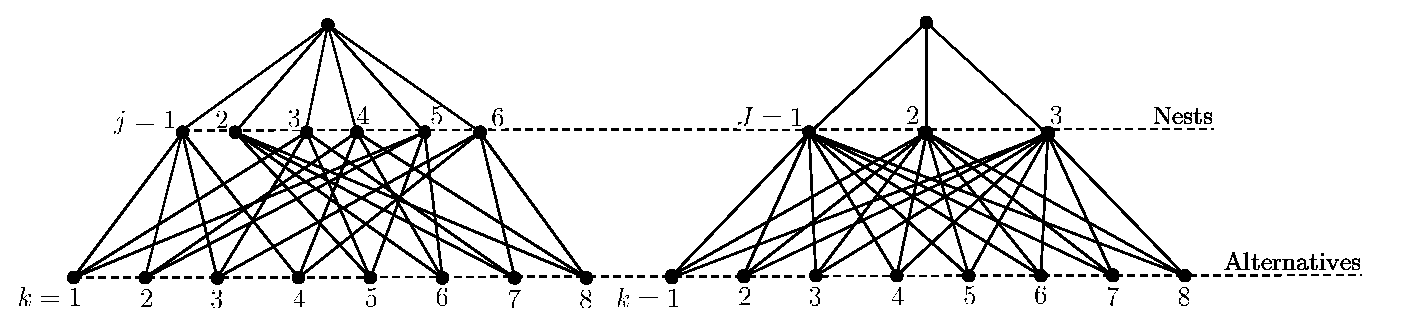
\includegraphics[width=160mm]{clip7-1.eps}
 \caption{集計問題生起例における GNL モデルの構造}
 \label{fig:7-1}
 \end{center}
\end{figure*}

\begin{table}
\begin{center}
\caption{選択構造例において最尤推定されたパラメータ} \label{tb:7-1}
\begin{tabular}{crcrcrcrcr}
\toprule\noalign{\smallskip}
Para.&Value&Para.&Value&Para.&Value&Para.&Value&Para.&Value
\\\noalign{\smallskip} \hline\hline
$\alpha_1$ & $-0.0147$ & $\gamma_{11}$ & $0.4760$ & $\gamma_{31}$ & $0.1038$ & $\gamma_{52}$ & $0.0061$ & $\gamma_{72}$ & $0.1604$\\
$\alpha_2$ &  $0.4755$ & $\gamma_{13}$ & $0.1149$ & $\gamma_{33}$ & $0.4621$ & $\gamma_{53}$ & $0.6821$ & $\gamma_{73}$ & $0.8396$\\
$\alpha_3$ &  $0.0021$ & $\gamma_{15}$ & $0.4091$ & $\gamma_{36}$ & $0.4341$ & $\gamma_{55}$ & $0.3118$ & $\gamma_{76}$ & $0.0000$\\
$\alpha_4$ & $-0.3597$ & $\gamma_{21}$ & $0.7870$ & $\gamma_{41}$ & $0.2955$ & $\gamma_{62}$ & $1.0000$ & $\gamma_{82}$ & $0.0357$\\
$\alpha_5$ & $0.8506$ & $\gamma_{24}$ & $0.1001$ & $\gamma_{44}$ & $0.0346$ & $\gamma_{64}$ & $0.0000$ & $\gamma_{84}$ & $0.1129$\\
$\mu$      & $0.4650$ & $\gamma_{25}$ & $0.1129$ & $\gamma_{46}$ & $0.6700$ & $\gamma_{65}$ & $0.0000$ & $\gamma_{86}$ & $0.8514$\\
\bottomrule
\end{tabular}
\end{center}
\end{table}

実際に集計化する上で,ネスト $1,2;3,4;5,6$ を集計化することを具体的に考えよう.
すなわち,図 \ref{fig:7-1} 右図の構造に集計化するものとする.
ここでは,
\vspace{3.0mm}
\begin{description}
\item [\mbox{}{\bf ルール 1 算術平均}] \mbox{}$ \check V_J^h = \frac{\sum_{j \in J} \check  V_j^h}{N_J}$,
\item [{\mbox{}\bf ルール 2 幾何平均}] \mbox{}$ \check V_J^h = \left(\prod_{j \in J} \check  V_j^h \right)^{1/N_J}$
\end{description}
\vspace{3.0mm}
の適用を試みる.ルール 1 は誰しもが一番最初に思いつくであろうもの,ルール 2 は効用項が $\exp$ の肩の上に乗っていることを反映したものである.
ここで,$\check V_j$ は,
\begin{align}
\check V_j^h := \sum \limits_{k^{\prime} \in {\cal K}_j} \left( \gamma_{k^{\prime}j}\exp \left({ V_{jk^\prime}^h + \hat V_{k^\prime}^h } \right) \right)^{1/\mu_j}
\end{align} 
である.$\check V_j^h$ と $\tilde V_{j}^h$,$V_j^{\prime h}$ の関係は,式\eqref{eq2-52} を参照せよ.また,$N_J$ は集計後のネスト $J$ に属する集計前のネスト $j$ の数である.

\begin{table}[t]
\begin{center}
\caption{間違った集計ルールの適用例} \label{tb:7-2}
\begin{tabular}{cccc}
\toprule
$j$ & $P_j^{\A}$ & $P_J^{\A}$(Rule 1) & $P_J^{\A}$(Rule 2)\\
\hline\hline
$1$& $0.239$ & \multirow{2}{3cm}{$0.324(5.2\%)^{\ast}$} & \multirow{2}{3cm}{$0.392(14.6\%)$} \\
$2$& $0.103$ &&\\
$3$& $0.303$ &\multirow{2}{3cm}{$0.376(16.8\%)$} & \multirow{2}{3cm}{$0.190(41.1\%)$} \\
$4$& $0.018$ &&\\
$5$& $0.196$ &\multirow{2}{3cm}{$0.300(10.8\%)$} & \multirow{2}{3cm}{$0.419(24.5\%)$} \\
$6$& $0.140$ &                                               &                                                \\
\hline
$k$ & $Q_k^{\A}$ & $Q_K^{\A}$(Rule 1) & $Q_K^{\A}$(Rule 2)\\
\hline \hline
$1$& $0.303$ & $0.326(7.9\%)$ & $0.404(33.5\%)$\\
$2$& $0.095$ & $0.091(4.8\%)$ & $0.109(14.6\%)$\\
$3$& $0.139$ & $0.131(6.0\%)$ & $0.129(8.3\%)$\\
$4$& $0.037$ & $0.028(25.4\%)$ & $0.038(2.4\%)$\\
$5$& $0.208$ & $0.242(16.5\%)$ & $0.174(16.4\%)$\\
$6$& $0.092$ & $0.049(53.0\%)$ & $0.063(31.9\%)$\\
$7$& $0.103$ & $0.119(15.3\%)$ & $0.064(38.2\%)$\\
$8$& $0.023$ & $0.014(37.6\%)$ & $0.020(13.9\%)$\\
\bottomrule
\multicolumn{4}{l}{$\ast$()内は集計前との相対誤差を表わす.}
\end{tabular}
\end{center}
\end{table}

それぞれ集計前,集計後の各選択肢,ネストの選択確率は表 \ref{tb:7-2}のとおりである.
ネスト $j$,商品 $k$ どちらのレベルにおいても,単純な算術平均や幾何平均による集計ルールは
選択割合(確率)の整合性がとれていないことがわかる.
特に,選択確率が小さい選択肢 $6$ の選択割合 $Q_6^{\A}$ は集計ルールの非整合性による影響が大きく,相対誤差がルール 1 では $53.0\%$,ルール 2 でも$31.9\%$ と大きくなっている.
つまり,整合的な集計ルールとは,算術,幾何平均のような単純なルールではない.

%****************************************************************************************************************************************
\section{集計ルールが満たすべき条件}
Sweet は集計が整合的に行われているために満たすべき条件として,MNL モデルのもとで,次の二つの条件を示している.
\begin{description}
\item [{\bf 条件 $1$ 固定需要}]  個人 $h$ が集計化された選択肢 $K$ を選ぶ周辺確率 $Q_K^h$ は,集計化前の選択肢 $k$ ($k$ は $K$ に包含されるものとする:$k \in K$)の効用 $V_k^h$ を
共通の効用である$V_{K}^{h}$に置き換えても変化がない.
\item  [\bf 条件 $2$ 選択確率の整合性] 個人 $h$ が集計化された選択肢 $K$ を選ぶ周辺確率 $Q_K^h$ は,集計化される前の選択肢 $k$ ($k \in K$) の選択確率と等しい:
\begin{equation}
Q_K^h = \sum \limits_{k \in K} Q_k^h.\label{eq7-1}
\end{equation}
\end{description}
これらの条件は,選択行動が $1$ 段階である MNL モデルの下での条件であることに留意されたい.
つまり,これをそのまま $2$ 段階の選択行動である NL,GNL の各モデルには適用できない.

Ivanova はこれらの条件を拡張し,NL モデルに適用している.
Ivanova では,ネスト $j$ について集計化しているモデルについて考えているが,
条件 $2$ をネスト $j$ 及び選択肢 $k$ について計 $2$ 回適用をしている.

本研究で対象とする GNL モデルでは,これ以外に,アロケーション・パラメータの条件が必要となる.
ここでは,次の条件を提示する:
\begin{description}
\item [{\bf 条件 $3$ アロケーション・パラメータの整合性}]
ネスト $j$ が $J$ に集計化された場合($j \in J$),アロケーション・ パラメータは次の条件を満たす必要がある:
\begin{equation}
\gamma_{kJ} = \sum_{j \in J} \gamma_{kj},\forall k. \label{eq7-2}
\end{equation}
\end{description}
条件 3 は集計が式\eqref{eq7-7}と整合的であるための条件である.
ただし,これはネストが集計化される場合についてのみの条件であり,選択肢が集計化される場合には適用することができない.

%****************************************************************************************************************************************
\section{GNL モデルにおける集計ルールの導出}
本節では,まず $1$ 回の集計を行なうブランド選択モデルにおいて,1) ネストの集計,2) 選択肢の集計,それぞれの場合について集計ルールを示し,
1) の拡張として,出発地,目的地計 $2$ 回の集計を行なう,3) 交通機関選択モデルにおけるネストの集計について集計ルールを示す.
なお,ここから先は,すべて消費者を表わす上添字 $h$ が付くため,これを省略する.

\subsection{ブランド選択モデル 1 :ネストの集計}
ここでは集計例と同様に,まずネストとして商品構成要素 $j$ を選択し,次に商品 $k$ を選択するものとする.
ネスト(商品構成要素)を $j \in J$という表現を用いよう.ここで $j$ は統合前のネスト,$J$ は統合後のネストを意味している.

ここで求めるべき集計ルールとは,$\hat V_J$,$\hat V_J^{\prime}$,$\hat V_{Jk}$ に関しての条件を指す.
条件 2 をネスト $j$ に適用し, GNL モデルの選択確率式\eqref{eq2-46}に代入することにより,
\begin{align}
\exp \left( \tilde V_J + V_J^{\prime} \right) =\sum \limits_{j \in J} \exp \left( \tilde V_j + V_j^{\prime} \right) \label{eq7-3}
\end{align}
を得る.ここで,条件 $1$ より
\begin{align}
V_J^{\prime} = \ln \sum_{j \in J} \exp V_j^{\prime}~~~~\forall j
\end{align}
であるため,式\eqref{eq7-3}は,
\begin{align}
\exp \left( \tilde V_J + V_J^{\prime} \right) =\sum \limits_{j \in J} \exp \left( \tilde V_j + V_J^{\prime} \right) \label{eq7-4}
\end{align}
と書き直せる.ここで,式\eqref{eq7-4}より $\tilde V_J$ に関する部分を消去し,
\begin{align}
\tilde V_J= \ln \sum_{j \in J} \exp \tilde V_j  \label{eq7-5}
\end{align}
を得る.式\eqref{eq7-5} を式\eqref{eq7-4} に代入し,これを整理することにより,
\begin{align}
V_J^{\prime}= \ln \sum_{j \in J} \exp \left(\tilde V_j + V_{j}^{\prime}\right) - \ln \sum_{j \in J} \exp \tilde V_j \label{eq7-6}
\end{align}
を得る.さらに条件 2 を結合確率 $\hat Q_k(j)$,$\hat Q_k(J)$ について適用する:
\begin{align}
\sum_{ j \in J} \hat Q_k(j) = \hat Q_k(J). \label{eq7-7}
\end{align}
ここで,結合確率 $\hat Q_k(j)$,$\hat Q_k(J)$ は,
\begin{align}
\hat Q_k(j):=& P_j P_{k|j}, \label{eq7-8}\\
\hat Q_k(J) :=& P_J P_{k|J} \label{eq7-9}
\end{align}
なる確率である.読者は,Ivanova の NL モデルへの適用例を見て,
\begin{align}
\hat Q_k(j):=& \sum_{J=1}^{N_J} \sum_{j \in J} P_j P_{k|j} ,\\
\hat Q_k(J):=& \sum_{J=1}^{N_J} P_J P_{k|J}
\end{align}
として条件 $2$ が適用されるのではないかと考えるかもしれない.
しかし,このような適用の場合,$V_{Jk}$ に関する条件を明示的には求めることができなくなる.

ここで条件 $2$ が適用されるのは,本質的には $P_{k|j}$,$P_{k|J}$ に関してであり,$j \rightarrow k$ という「選択経路」ごとに集計ルールが適用されるべきである.
データとして $j$ が観測可能か否かに限らず,集計ルールとして「選択経路」ごとの整合性が必要である.
集計前の選択肢において $\hat P_j$ は計算されており,これと整合的に $P_J$ も計算される.
つまり,$Q_k$ について整合的であるルールは,$P_{j}$,$\P_{J}$ と $P_{k|j}$,$P_{k|J}$ がマルコフ性を有するため,残りの $P_{k|j}$,$P_{k|J}$ に関して整合的である必要がある.
これはブランド選択モデルだけではなく,交通機関選択モデルの出発地側も同様である.

式\eqref{eq7-7}は
\begin{align}
P_J P_{k|J} = \sum_{j \in J} P_j P_{k|j} \Longleftrightarrow P_{k|J} = \frac{\sum_{j \in J} P_j P_{k|j}}{\sum_{j^{\prime} \in J} P_{j^{\prime}}}\label{eq7-10}
\end{align}
と修正される.
式\eqref{eq7-10} は
\begin{align}
P_{k|J} = & \frac{\left( \gamma_{kJ}\exp \left( { V_{Jk}} + \hat V_{k} \right) \right)^{1/\mu_J}}
{\sum \limits_{k^{\prime} \in N_J} \left( \gamma_{k^{\prime}J}\exp \left( {V_{Jk^\prime}} + \hat V_k \right) \right)^{1/\mu_J}} 
= \frac{\left( \gamma_{kJ} \exp \left( V_{Jk} + \hat V_{k} \right) \right)^{1/\mu_J}}{\left( \exp V_J^{\prime} \right)^{1/\mu_J}}\notag\\
= & \frac{\sum_{j \in J} P_j P_{k|j}}{ \sum_{j^{\prime} \in J} P_{j^{\prime}}} \label{eq7-11}
\end{align}
と等価である.式\eqref{eq7-11}について対数を取り,$1/\mu_J$ で除すことにより,
\begin{align}
V_{Jk} = V_J^{\prime} - \hat V_k + \mu_J \ln \left( \frac{\sum_{j \in J} P_j P_{k|j}}{ \gamma_{kJ}^{1/\mu_J} \sum_{j^{\prime} \in J} P_{j^{\prime}}} \right)  \label{eq7-12}
\end{align}
を得る.最後に条件 $3$ を式\eqref{eq7-12}に代入し,
\begin{align}
V_{Jk} =& V_J^{\prime} - \hat V_k + \Upsilon, \label{eq7-13}\\
\Upsilon :=& \mu_J \ln \left( \frac{\sum_{j \in J} P_j P_{k|j}}{ \left( \sum_{j \in J} \gamma_{kj} \right)^{1/\mu_J} \sum_{j^{\prime} \in J} P_{j^{\prime}}} \right)  \label{eq7-14}
\end{align}
となる.

これらの式のうち,式\eqref{eq7-5},\eqref{eq7-6},\eqref{eq7-13}が,GNL モデルにおけるネストを集計した場合の満たすべき集計ルールとなる.
ここで注意すべきは,$\gamma_{kJ}$ と異なり,$\mu_J$ に関するルールは導出されないという点である.
これは,ネストごとの類似度パラメータが同一($\mu_J = \mu_j := \mu~~\forall j,J$)でない限り,集計後に新たに最尤推定もしくはその他の方法,ルールでパラメータ設定をしなければならないことを意味している.
%%%%%%%%%%%%%%%%%%%%%%%%%%%%%%%%%%%%%%%%%%%%%%%%%%%%%%%%%%%%%%%%%%%%%%%%%%%%%%%%%%%%%%%%%%%%%%%%%%%%%%%%%%%%%%%%%%%%%%%%%%%%%%%%%%%%%%%%%%%%%%%%%%%%%%%%%%%%%%%%%%%%%%%%%%%%%%%%%%%%%%%
\subsection{ブランド選択モデル 2 :選択肢の集計}
次に,ネストを構成する商品構成要素を集計するのではなく,選択肢であるブランドを集計する場合を考える.
ネストの集計と同様に,選択肢(ブランド)を $k \in K$ という表現を用いよう.ここで $k$ は統合前の選択肢,$K$ は統合後の選択肢を意味している.

ネストを集計した場合は,$\tilde V_J$,$V_J^{\prime}$,$\hat V_{Jk}$ に関しての条件三つが必要であったが,今回は $\hat V_{jK}$,$\hat V_K$ に関しての二つとなる.
条件 2 を$\hat P_{k|j}$,$\hat P_{K|j}$に適用することにより,
\begin{align}
&\left( \gamma_{Kj}\exp \left( V_{jK} + \hat V_K \right) \right)^{1/\mu_j} = \sum \limits_{k \in K} \left( \gamma_{kj} \exp \left( { V_{jk} + \hat V_k } \right) \right)^{1/\mu_j}\label{eq7-15}
\end{align}
を得る.ここで,条件 1 より,
\begin{align}
&\left( \gamma_{Kj} \exp \left( V_{jK} + \hat V_K \right) \right)^{1/\mu_j} = \sum \limits_{k \in K} \left( \gamma_{kj} \exp \left( { V_{jK} + \hat V_k } \right) \right)^{1/\mu_j}\label{eq7-16}
\end{align}
となる.式\eqref{eq7-16} を $\hat V_{K}$ について解くと,
\begin{align}
\hat V_{K} = \mu_j \ln \frac{1}{\gamma_{Kj}} \left( \sum \limits_{k \in K} \left( \gamma_{kj} \exp \hat V_{k} \right)^{1/\mu_j} \right) \label{eq7-17}
\end{align}
を得る.ちなみに式\eqref{eq7-17} の条件は,$\hat P_j^{\prime}$ に条件 $1$ を適用しても同様に得られる.
次に,式\eqref{eq7-17} を式\eqref{eq7-15} に代入し,整理すると,次の条件を得る:
\begin{align}
V_{jK} &= \mu_j \ln \left( \frac{1}{\gamma_{Kj}} \sum \limits_{k \in K} \left( \gamma_{kj} \exp V_{jk} \right)^{1/\mu_j} \right) - \mu_j \ln \left( \frac{1}{\gamma_{Kj}} \sum \limits_{k \in K} \left( \gamma_{kj} \exp \hat V_{k} \right)^{1/\mu_j} \right).  \label{eq7-18}
\end{align}

これらの式のうち,式\eqref{eq7-17},\eqref{eq7-18} が,GNL モデルにおけるブランド選択モデルでネストを集計した場合の満たすべき集計ルールとなる.
選択肢を集計化した場合には,ネストを集計化した場合のようなアロケーション・パラメータに関するルールは存在しない.
そのため,集計化に伴なう新たなパラメータ推定を行なうことを避ける意味において,説明変数により構造化した構造化 GNL モデル\cite{PB99} のような形で,アロケーション・パラメータを集計前に推定することが望ましい.
%%%%%%%%%%%%%%%%%%%%%%%%%%%%%%%%%%%%%%%%%%%%%%%%%%%%%%%%%%%%%%%%%%%%%%%%%%%%%%%%%%%%%%%%%%%%%%%%%%%%%%%%%%%%%%%%%%%%%%%%%%%%%%%%%%%%%%%%%%%%%%%%%%%%%%%%%%%%%%%%%%%%%%%%%%%%%%%%%%%%%%%
\subsection{交通機関選択モデル}
ここでは,まずネストとして目的地のゾーン $d$ を選択し,次に交通機関 $k$ を選択するモデルを考える.
交通計画分野に精通していない方にとっては,この選択構造(順番)は奇異に映るかもしれないが,
四段階推計法 (例えば\cite{Dob98}) のステップに準拠したものである.
当然,各交通機関の効用にはその交通機関により行くことが出来る目的地の効用が説明変数として加わることとなる.

交通機関選択モデルの場合,集計化された選択人数は出発地のゾーン $o$ ,目的地のゾーン $d$ を用い,
\begin{align}
H_k^o=&H^o Q_k^o = H^o  \sum_{d^{\prime}=1}^{N_d} \left( \frac{ \exp \left(\tilde V_{d^{\prime}}^o + V_{d^{\prime}}^{\prime o} \right)}
{\sum \limits_{d^{\prime \prime}=1}^{N_d} \exp \left(\tilde V_{d^{\prime \prime}}^o + V_{d^{\prime \prime}}^{\prime o} \right) }  \frac{\left( \gamma_{kd^{\prime}} \exp \left( V_{d^{\prime}k}^o + \hat V_{k}^o \right) \right)^{1/\mu_{d^{\prime}}}}
{\sum \limits_{k^{\prime} \in N_{d^{\prime}}} \left( \gamma_{k^{\prime}d^{\prime}} \exp \left(V_{d^{\prime}k^{\prime}}^{o} + \hat V_{k^{\prime}}^o \right) \right)^{1/\mu_{d^{\prime}}}} \right) \label{eq7-19}
\end{align}
と修正される.ここで, $H_k^o$ はゾーン $o$ において交通機関 $k$ を利用する人数,$H^o$ はゾーン $o$ を出発地とする人数,$Q_k^o$ はゾーン $o$ における交通機関 $k$ の選択確率であり,
式\eqref{eq7-1}--\eqref{eq7-7}と対応する部分についても上添字 $o$ がつく.
式\eqref{eq7-19}の意味するところは,交通機関選択モデルにおいては,選択確率における選択肢だけではなく,ゾーンの人数 $H^o$ についても集計化されるということである.
つまり,ブランド選択モデルで示した集計ルールはそのまま適用することができない.

前節までと同様に,ゾーンの集計化を $o \in O$,$d \in D$という表現を用いよう.ここで $o, d$ はネストを統合前,$O, D$ はネスト統合後のゾーンであり,
それぞれ $o, d$ は $O, D$ に統合(集計)されることを意味している.

さて,我々は,式\eqref{eq7-19}と同様の
\begin{align}
H_k^O=&H^I  \sum_{D^{\prime}=1}^{N_D} \left( \frac{ \exp \left(\tilde V_{D^{\prime}}^O + V_{D^{\prime}}^{\prime O} \right)}
{\sum \limits_{D^{\prime \prime} =1}^{N_D} \exp \left(\tilde V_{D^{\prime \prime}}^{O} + V_{D^{\prime \prime}}^{\prime O} \right) } \frac{\left( \gamma_{kD^{\prime}}\exp \left( V_{D^{\prime}k}^{O} + \hat V_{k}^{O} \right) \right)^{1/\mu_{D^{\prime}}}}
{\sum \limits_{k^{\prime} \in {\cal K}_{D^{\prime}}} \left( \gamma_{k^{\prime}D^{\prime}} \exp \left( V_{D^{\prime}k^{\prime}}^{O} + \hat V_{k^{\prime}}^{O} \right) \right)^{1/\mu_{D^{\prime}}}} \right) \label{eq7-20}
\end{align}
に関して集計化された場合の $O, D$における確定的効用 ($V_D^O, V_D^{\prime O}, V_{Dk}^O$) に関する集計ルールを見つけたい.
ここで,$V_D^{\prime O}$ は以下の式で表される効用である:
\begin{align}
V_D^{\prime O}:=\mu_D \ln  \sum \limits_{k^{\prime} \in {\cal K}_D} \left( \gamma_{k^{\prime}D} \exp \left( V_{Dk^{\prime}}^{O} + \hat V_{k^{\prime}}^{O} \right) \right)^{1/\mu_{\it D}}.
\end{align}

Ivanova と同様に,まず 目的地 $d$ についてのみ集計化しよう.
目的地側の集計ルールは,ブランド選択モデルにおいてネストを集計した場合と同様に,
\begin{align}
\tilde V_D^o &= \ln  \sum_{d \in D} \exp \hat V_d^o , \label{eq7-21}\\
V_D^{\prime o} &= \ln \sum_{d \in D} \exp \left(\hat V_d^o + \hat V_{d}^{\prime o} \right) - \ln \sum_{d \in D} \exp \hat V_d^o , \label{eq7-22}\\
V_{Dk}^o &= V_D^{\prime o}  - \hat V_k^o + \mu_D \ln \left( \frac{\sum_{d \in D} P_d^o P_{k|d}^o }{ \left( \sum_{d \in D} \gamma_{kd} \right)^{1/\mu_D} \sum_{d^{\prime} \in D} P_{d^{\prime}}^o } \right) \label{eq7-23}
\end{align}
となる.ここでブランド選択モデルとの違いは,添字 $o$ がつく点以外には存在しない.

次に出発地側の満たすべき集計ルールを示そう.条件 1 を $\tilde V_D^{o}$,$V_D^{\prime o}$ に適用し,
\begin{align}
\exp \left(\tilde V_D^O+ V_D^{\prime O} \right) &= \sum_{o \in O} \frac{H^o}{H^O}  \exp \left(\tilde V_D^o + V_D^{\prime o} \right) = \sum_{i \in I} \frac{H^o}{H^{O}} \exp \left(\tilde V_D^O + V_D^{\prime O} \right)
\end{align}
を得る.ここから目的地側と同様に,
\begin{align}
\tilde V_D^O &= \ln \sum \limits_{o \in O} \left( \frac{H^o}{H^O} \exp \tilde V_D^o \right),  \label{eq7-24}\\
V_D^{\prime O} &= \ln \sum \limits_{o \in O} \left( \frac{H_o}{H_O} \exp \left( \tilde V_D^o + V_D^{\prime o} \right) \right) - \ln \sum \limits_{o \in O} \left( \frac{H_o}{H_O} \exp \tilde V_D^o \right)  \label{eq7-25}
\end{align}
を得る.さらに,標本抽出理論を条件付き確率 $ P_{k|D}^O $ に適用すると,
\begin{align}
P_{k|D}^O = \frac{\hat Q_k^O (D)}{P_d^O} = \frac{ \sum_{o \in O} \frac{H_o}{H_O}  \hat Q_k^o (D)}{ \sum_{o \in O} \frac{H_o}{H_O} P_D^o }\label{eq7-26}
\end{align}
と書き表わされる.これは,目的地側と同様に,
\begin{align}
P_{k|D}^O = & \frac{\left( \gamma_{kD}\exp \left( V_{Dk}^O + \hat V_{k}^O \right) \right)^{1/\mu_D}}
{\sum \limits_{k^{\prime} \in {\cal K}_D} \left( \gamma_{k^{\prime}D}\exp \left( V_{Dk^{\prime}}^O + \hat V_{k^{\prime}}^{O} \right) \right)^{1/\mu_D}} \notag\\
= & \frac{\left( \gamma_{kD}\exp \left( V_{Dk}^{O} + \hat V_{k}^O \right) \right)^{1/\mu_D}}
{\left( \exp V_D^{\prime O} \right)^{1/\mu_D}} =  \frac{ \sum_{o \in O} H_o  \hat Q_k^o (D)}{ \sum_{o \in O} H_o  P_D^o } \label{eq7-27}
\end{align}
と等価である.式\eqref{eq7-27}について対数を取り,$1/\mu_D$で除すことにより,
\begin{align}
V_{Dk}^O &= V_D^{\prime O}  - \hat V_{k}^{O} + \mu_D \ln \left( \frac{ \sum_{o \in O} H_o \hat Q_k^o (D)}{ \left( \sum_{d \in D} \gamma_{kd} \right)^{1/\mu_D} \sum_{o^{\prime} \in O} H_{o^{\prime}} P_D^{o^{\prime}} } \right)  \label{eq7-28}
\end{align}
を得る.
これらの式のうち,式\eqref{eq7-23},\eqref{eq7-24},\eqref{eq7-27}が,GNL モデルにおける出発地側の満たすべき集計ルールとなる.

出発地,目的地あわせ,式\eqref{eq7-21}--\eqref{eq7-23},\eqref{eq7-24},\eqref{eq7-25},\eqref{eq7-28}が全体として満たすべき集計ルールである.
%****************************************************************************************************************************************
\section{MNL,NL モデルとの集計ルールの比較}
本節では,前節で導出されたブランド選択モデルにおける集計ルールを MNL,NL モデルと比較する.
ネストを集計した場合と選択肢を集計した場合では,MNL,NL,GNL モデルというモデル拡張の順番と特徴の出現が異なるため,別々に比較する.

\subsection{ネストを集計した場合}
ネストを集計した場合の集計ルールを表 \ref{tb:7-3}に示す.
以下では,モデルの比較を行なうため,同じ条件でもモデルを特定する必要がある場合には,$\tilde V_{j|{\rm NL}}$ とモデル名を明記した表記を用いることがある.

まず,各モデルにおける集計ルールを比較する.
ネストを集計した場合には, $\tilde V_j$ に関するルールには,MNL,NL,GNL の各モデル間で変化がない.
これは,NL,GNL モデルの ネスト選択時の構造が MNL モデルのそれと同じく,アロケーション・パラメータが肩の上にかかっていたり,類似度パラメータが加わっていないため,
これらが式中に現れないためである.
同様に,MNL モデルにおける $V_{jk}$,NL,GNL モデルにおける $V_{j}^{\prime}$ も同様である.ただし,MNL モデルにおいては,$j$,$k$ に相当する部分が 1 段階の選択に集約されているため,
NL,GNL モデルでは現れない $-\hat V_k$ の項が現われる.MNL モデルにおける $V_{j}^{\prime}$ に関する条件と,NL,GNL モデルにおける $V_{jk}$ に関する条件の同型性から,
ログサム $V_{j}^{\prime} $ は $V_{jk}$ に端を発する項であることがわかる.非常に荒っぽい表現となるが,MNL モデルにおける $V_{jk}$ に関する条件は,NL,GNL モデルにおいては $V_{j}^{\prime}$,$V_{jk}$ に分離することとなる.
そして,最後の $V_{jk}$ についてはモデルにより加わる項が異なる.
この事実から,さらにネストを重ねたモデルや GNL モデルにさらにネストを付加したもの (高橋・大野,2001 \cite{TO11};Koppelman and Sethi,2005 \cite{KS05}) では,この項のみが変化するものと容易に推測できる.
これは,NL,GNL モデルの $V_{jk}$ に関する条件に含まれる $V_{j}^{\prime}$ についてその集計ルールの条件を代入し,整理すると,異なるのが最後の項 ($\Upsilon$) のみとなる.

次に,集計により各確定的効用項がどのように変化するのかを示そう.
どのモデルにおいても,$\tilde V_J$ については,Sweet でいうセントラル・ログサムにあたる.
従って,Sweet の式 (12) と同様に,
\begin{align}
\min \limits_{j \in J} \tilde V_j \leq \tilde V_J \leq \max \limits_{j \in J} \tilde V_j 
\end{align}
となる.$\tilde V_J^{\prime}$ についても同様に,
\begin{align}
&\min \limits_{j \in J} \left( \tilde  V_j + V_j^{\prime} \right) - \max \limits_{j \in J} V_j^{\prime} \leq V_J^{\prime} \leq \max \limits_{j \in J} \left(\tilde V_j + V_j^{\prime} \right) - \min \limits_{j \in J} V_j^{\prime} \label{eq7-29}
\end{align}
を得る.$ V_{Jk}$ については,$V_J^{\prime}$ は式\eqref{eq7-29} に示すとおりであり,$\hat V_k$ は集計と無関係であるため定数である.
従って,$ V_{Jk}$ の上限,下限は最後の項 $\Upsilon$ に左右される.
$\Upsilon$ は,$P_{k|j}$ を $P_{j}$ で重み付けしたものを $\mu_j$ 乗したものを,$\gamma_{kJ}$ で除し,対数をとったものである:
\begin{align}
\Upsilon = \ln \left( \frac{1}{\sum_{j \in J} \gamma_{kj}} \left( \frac{\sum_{j \in j} P_{k|j} P_j}{\sum_{j^{\prime} \in J} P_{j^{\prime}}} \right)^{\mu_j} \right).
\end{align}
ここで,式\eqref{eq7-6},\eqref{eq7-7} より,
\begin{align}
0 \leq \sum_{j \in J} \gamma_{kj} = \gamma_{kJ} \leq 1 \label{eq7-30}
\end{align}
である.
\begin{landscape}
\begin{center}
\begin{table}
\caption{MNL, NL, GNL モデルにおける集計ルール:ネスト $j$ を集計する場合} \label{tb:7-3}
\begin{tabular}
{p{2.0cm}p{3.9cm}p{7.7cm}p{9.0cm}}
\toprule
\multicolumn{1}{c}{Model} & \multicolumn{1}{c}{$\tilde V_{J}$} & \multicolumn{1}{c}{$ V_{J}^{\prime}$} & \multicolumn{1}{c}{$ V_{Jk}$} \\
\noalign{\smallskip}\hline\hline\noalign{\smallskip}
\multicolumn{1}{c}{ } & & &\\
\multicolumn{1}{c}{MNL} &$\tilde V_{J} = \ln \sum \limits_{j \in J}  \exp \tilde V_{j} $
& \multicolumn{1}{c}{---}
& $V_{Jk} = \ln \sum \limits_{j \in J}  \exp V_{jk} - \ln \sum \limits_{j \in J} \exp \tilde V_{j} - \hat V_k $\\
\multicolumn{1}{c}{ } & & &\\
\multicolumn{1}{c}{NL} & $\tilde V_J= \ln \sum \limits_{j \in J} \exp \tilde V_j $
& $V_J^{\prime} = \ln \sum \limits_{j \in J} \exp \left(\tilde V_j + V_{j}^{\prime} \right) - \ln \sum \limits_{j \in J} \exp \tilde V_j $
& $V_{Jk} = V_J^{\prime} - \hat V_k + \mu_J \ln \left( \frac{\sum_{j \in J} P_j P_{k|j}}{ \sum_{j^{\prime} \in J} P_{j^{\prime}}} \right) $\\
\multicolumn{1}{c}{ } & & &\\
\multicolumn{1}{c}{GNL} & $\tilde V_J= \ln \sum \limits_{j \in J}  \exp \hat V_j  $
& $V_J^{\prime} = \ln \sum \limits_{j \in J} \exp \left(\tilde V_j + V_{j}^{\prime} \right) - \ln \sum \limits_{j \in J} \exp \tilde V_j $
& $V_{Jk} = V_J^{\prime} - \hat V_k + \mu_J \ln \left( \frac{\sum_{j \in J} P_j P_{k|j}}{ \left( \sum_{j \in J} \gamma_{kj} \right)^{1/\mu_J} \sum_{j^{\prime} \in J} P_{j^{\prime}}} \right) $\\
\multicolumn{1}{c}{ } & & &\\
\bottomrule
\end{tabular}\\
\end{table}
\end{center}
\end{landscape}
\begin{landscape}
\begin{center}
\begin{table}
\caption{MNL, NL, GNL モデルにおける集計ルール:選択肢 $k$ を集計する場合} \label{tb:7-4}
\begin{tabular}
{p{2.0cm}p{7.0cm}p{14.0cm}}
\toprule
\multicolumn{1}{c}{Model} & \multicolumn{1}{c}{$\hat V_{K}$} & \multicolumn{1}{c}{$V_{jK}$} \\
\noalign{\smallskip}\hline\hline\noalign{\smallskip}
\multicolumn{1}{c}{ } & & \\
\multicolumn{1}{c}{MNL} &$\hat V_{K} = \ln \sum \limits_{k \in K}  \exp \hat V_{k} $
& $V_{jK} = \ln \sum \limits_{k \in K} \exp V_{jk} - \ln \sum \limits_{k \in K}  \exp \hat V_{k} - \tilde V_j $ \\
\multicolumn{1}{c}{ } & & \\
\multicolumn{1}{c}{NL$^{*}$} & $\hat V_{K} = \mu_j \ln \sum \limits_{k \in K} \left( \exp \hat V_{k} \right)^{1/\mu_j}  $ 
& $V_{jK} = \mu_j \ln \sum \limits_{k \in K} \left( \exp V_{jk} \right)^{1/\mu_j} - \mu_j \ln \sum \limits_{k \in K} \left( \exp \hat V_{k} \right)^{1/\mu_j} $ \\
\multicolumn{1}{c}{ } & & \\
\multicolumn{1}{c}{GNL} &$\hat V_{K} = \mu_j \ln \left( \frac{1}{\gamma_{Kj}} \sum \limits_{k \in K} \left( \gamma_{kj} \exp \hat V_{k} \right)^{1/\mu_j} \right)$ 
&$V_{jK} = \mu_j \ln \left( \frac{1}{\gamma_{Kj}} \sum \limits_{k \in K} \left( \gamma_{kj} \exp V_{jk} \right)^{1/\mu_j} \right) - \mu_j \ln \left( \frac{1}{\gamma_{Kj}} \sum \limits_{k \in K} \left( \gamma_{kj} \exp \hat V_{k} \right)^{1/\mu_j} \right) $\\
\multicolumn{1}{c}{ } & & \\
\bottomrule
\end{tabular}\\
$^{*}$ Ivanova をはじめ,既存研究では,NL モデルにおいて選択肢を集計した場合を求めているものはない.今回は GNL モデルの場合と同様に求めた.
\end{table}
\end{center}
\end{landscape}
\noindent
一般的に $\gamma_{kJ}$ が大きい場合,つまり多くのネストを束ねた場合,$\Upsilon$ はマイナスになりやすくなる. 
また,式\eqref{eq7-5},$0 \leq P_j \leq 1$,$0 \leq P_{k|j} \leq 1$より,
\begin{align}
0 \leq \left( \frac{\sum_{j \in J} P_j P_{k|j}}{ \sum_{j^{\prime} \in J} P_{j^{\prime}}} \right)^{\mu_j} \leq 1 \label{eq7-31}
\end{align}
である.
一般的に $P_{k|j}$ が大きい場合,つまりネスト $j$ に属する選択肢が魅力的な場合,$\Upsilon$ はプラスになりやすくなる.
最終的な $\Upsilon$ の正負は式\eqref{eq7-30},\eqref{eq7-31}の大小で決まる.
しかし,$\Upsilon$ の最大値,最小値は決めることはできず,$V_{Jk}$ についても同様となる.

最後に,各モデルの選択確率 (Wen and Koppelman) と,各モデルのネストの集計ルールにおける条件間は整合的であることを示そう.
$\mu_J\rightarrow 0$ とすると,NL モデルの場合の $\hat V_{Jk}$ に関する条件は,
\begin{align}
V_{Jk|{\rm NL}} =& V_J^{\prime} - \hat V_k = \ln \sum \limits_{j \in J}  \exp V_{jk} - \ln \sum \limits_{j \in J} \exp \tilde V_{j} - \hat V_k = V_{Jk|{\rm MNL}} 
\end{align}
となり,NL モデルの条件は MNL モデルのそれに帰着する.同様に,$\gamma_{kj}\rightarrow 1$ とすると GNL モデルにおける $\hat V_{Jk}$ に関する条件は,
\begin{align}
V_{Jk|{\rm GNL}} =& V_J^{\prime} - \hat V_k + \mu_J \ln \left( \frac{\sum_{j \in J} P_j P_{k|j}}{ \left( \sum_{j \in J} 1 \right)^{1/\mu_J} \sum_{j \in J} P_j} \right) \notag\\
=& V_J^{\prime} - \hat V_k + \mu_J \ln \left( \frac{\sum_{j \in J} P_j P_{k|j}}{ \sum_{j \in J} P_j} \right) = V_{Jk|{\rm NL}} 
\end{align}
となり,GNL モデルの条件は NL モデルのそれに帰着する.
$V_J$ 及び $V_{j}^{\prime}$ に関する条件は NL モデルと GNL モデルで同じであるため,各モデルにおける選択確率の関係性と,ネストの集計ルールの条件の関係性は整合的であるといえる.

\subsection{選択肢を集計した場合}
次に,選択肢を集計した場合の集計ルールを表 \ref{tb:7-4}に示す.
まず,ネストを集計した場合と同様に,各モデルにおける集計ルールを比較する.
$\hat V_K$ に関する条件は,各モデルのログサムそのものである.
$V_{jK}$ に関しても,$V_{jk}$ のログサムから $\hat V_k$ のログサムを差し引いたものとなる.
ただし,MNL モデルでは,NL,GNL の各モデルにおいてネスト段階の効用となる $\tilde V_j$ が差し引かれる.
これは,ネスト $j$ を与件とすれば,$k$ の選択は,NL,GNL モデルともに MNL モデルと同様となるためである.

当然各項の集計による効用の変化は,ネストを集計した場合と同様に,次のとおりとなる:
\begin{align}
&\min \limits_{k \in K} \hat V_{k|{\rm NL}} \leq \hat V_{k|{\rm NL}} \leq \max \limits_{k \in K} \hat V_{k|{\rm NL}},\\
&\min \limits_{k \in K} \gamma_{kj} \hat V_{k|{\rm GNL}} \leq \gamma_{Kj} \hat V_{k|{\rm GNL}} \leq \max \limits_{k \in K} \gamma_{kj} \hat V_{k|{\rm GNL}},\\
&\min \limits_{k \in K} V_{jk|{\rm NL}} - \max \limits_{k \in K} \hat V_{k|{\rm NL}} \leq V_{jK|{\rm NL}} \leq  \max \limits_{k \in K} V_{jk|{\rm NL}} - \min \limits_{k \in K} \hat V_{k|{\rm NL},} \\
&\min \limits_{k \in K} \gamma_{kj} V_{jk|{\rm GNL}} - \max \limits_{k \in K} \gamma_{kj} \hat V_{k|{\rm GNL}} \leq \gamma_{Kj} V_{jK|{\rm GNL}} \leq \max \limits_{k \in K} \gamma_{kj} V_{jk|{\rm GNL}} - \min \limits_{k \in K} \gamma_{kj} \hat V_{k|{\rm GNL}}.
\end{align}

選択肢を集計した場合にも,モデルの選択確率と,集計ルールとの間には整合性が保たれる.
$\mu_J\rightarrow 1$ とすると,NL モデルの場合の $V_{jK}$ に関する条件は,
\begin{align}
V_{jK|{\rm NL}} &= \ln \sum \limits_{k \in K} \left( \exp V_{jk} \right)^{1/1} - \ln \sum \limits_{k \in K} \left( \exp \hat V_{k} \right)^{1/1} =\ln \sum \limits_{k \in K} \exp V_{jk} - \ln \sum \limits_{k \in K} \exp \hat V_{k} 
\end{align}
となる.ここで,NL モデルから MNL モデルへの帰着は,2 段階から 1 段階の選択構造に変化するため,ネスト選択における効用項 $\hat V_j$ が現われる.ただし,$\hat V_j$ は,$k$ に関する集計とは無関係であるため,ここでは定数である.
そのため,それを差し引く形で NL モデルの条件は MNL モデルの条件に帰着する.同様に,$\gamma_{kj}\rightarrow 1$ とすると GNL モデルの場合の $\hat V_{jK}$ に関する条件は,
\begin{align}
V_{jK|{\rm GNL}} =& \mu_j \ln \left( \frac{1}{1} \sum \limits_{k \in K} \left( 1 \exp V_{jk} \right)^{1/\mu_j} \right) - \mu_j \ln \left( \frac{1}{1} \sum \limits_{k \in K} \left( 1 \exp \hat V_{k} \right)^{1/\mu_j} \right) \notag\\
= & V_{jK|{\rm NL}} 
\end{align}
となり,GNL モデルの条件は NL モデルの条件に帰着する. $\hat V_{K}$ についても同様に示すことができる. 
従って,選択肢の集計ルールにおける各条件の関係性についても,各モデルの選択確率 \cite{WK01} の関係性と整合的であるといえる.
%****************************************************************************************************************************************
\section{7 章のまとめ}
本章では,複数の要素間の相関を考慮可能な Generalized Nested Logit (GNL) モデルについて,集計問題を克服可能な集計ルールを導出した.
まず,集計問題が GNL モデルにおいて実際に生起することを,スキャン・パネル・データより推定した GNL モデルを用い,ネストを集計することにより,その前後で選択確率が整合的であるかを確かめた.
このとき,特に算術平均,幾何平均といった単純な集計ルールではその差が大きいことを示した.
次に GNL モデルにおいて用いるべき集計ルールが満たすべき条件を示した.
具体的には,Sweet の条件にアロケーション・パラメータの条件を追加した.
この導出した集計ルールを用いて, GNL モデルにおいてその集計問題が克服可能な条件を,
ブランド選択モデルにおいて,1) ネストを集計した場合,2) ブランドを選択した場合,2 段階の集計がある交通機関選択モデルにおいて 3) ネストを集計した場合,
それぞれについて集計問題を回避する集計ルールを導出した.
この際に,GNL モデルにおいては,集計ルールが満たすべき条件の適用を,Ivanova が示した周辺確率ごとではなく,ネストと選択肢のそれぞれの選択の結合確率ごとにすべきことを明らかにした.

さらに,集計ルールをブランド選択モデルを例に,1) ネストを集計した場合,2) 選択枝を集計した場合,それぞれについて MNL,NL,GNL の各モデル間で比較し,その性質を明らかにした.
その結果,次に示すことがわかった; 1) 各モデルの選択確率と集計ルールは整合性,2) 限定的ではあるがほぼ全ての場合において,集計化された各確定的効用項には,最大値,最小値が存在.
1) については, GNL モデルは MNL,NL,PCL の各モデルを内包しているため,GNL において得られた集計ルールをもとに,これらのモデルの集計ルールを容易に得られることを意味している.
2)については,実際に分析者が集計を行なう際に,集計が整合的に行なわれたかを確かめる際に用いることができる.

これらの事実及び集計ルールは,複数のモデル間の整合性を図る上で非常に有意義なことである.
特に GNL モデルでは,モデルの構造上選択肢の複数のネストへの帰属を許すため,ネスティングの方法により選択肢そのものの概念が大きく異なることが予想される.
また,選択肢数,ネスト数の増加は,類似度パラメータ,アロケーション・パラメータの著しい増加につながる.
このパラメータの増加は,パラメータ推定時の次元の増加だけではなく尤度関数の多峰性を増すことになる.
そのため,分析対象に適したネスティング,選択肢の定義,集計を行なう必要性がある.
例えば,マーケット・シェアの低い商品は「その他」という選択肢に束ねることが多くのマーケティングの研究で行なわれている.
そのような場合には,今回導いたルールを用いることは,分析者にとって計算量を減らし,同時にモデル間の整合性を保つために非常に有益であろう.




%\chapter{結論}
%----------------------------
\section{本研究のまとめ}
%----------------------------
本研究では,複雑な選択肢間の異質性を考慮できる Generalized Nested Logit (GNL) モデルについて
基本的な性質を明らかにし,マーケティング分野において適用,拡張,及び効率的利用のためのツールの開発を行なった.
本研究で明らかになった成果は次のとおりである.

2 章では,GNL モデルが持つ,集計的,非集計的な側面からの情報理論との対応付けを行なった.
その結果,次のことがわかった:
\begin{enumerate}
\item GNL モデルは集計的に,エントロピー制約付き社会的効用最大化問題として解釈可能,
\item 集計的なモデルにおいて,サンプル数を $1$ とすると個人レベルでの効用最大化問題として解釈可能,
\item GNL モデルの段階的最尤推定問題は,その各段階がそれぞれ共役なエントロピー最大化(情報量最小化)問題と等価,
\item 一般的に効用最大化と整合的であるためとされたパラメータの制約条件は,情報整合的な制約と,効用最大化と整合的であるための条件があることが判明.
\end{enumerate}
これらの事実により,新たなパラメータ推定の方法や,パラメータの制約条件の付加の仕方が提案され,情報理論的な GNL モデルの解釈が可能となった.

3 章では,従来ほとんど例がなかった GNL モデルのマーケティング分野への適用を行なった.
具体的な GNL モデルの構造を決定するネスティング・ルールとして,要素分割を提案し,商品カテゴリーとしてコーラに対し,適用,検証を行なった.
その結果,次のことがわかった:
\begin{enumerate}
\item MNL,NL,GNL の各モデルを比較し,各基本統計量において,GNL モデルが優位,
\item 集計した選択割合においても,GNL モデルが優位,
\item 上記のモデル間には,効用関数パラメータの大きな相違が見られる.
\end{enumerate}
4 章では,3 章で提案した GNL モデルの適用を,消費者に異質性について考慮できるように拡張した LGNL モデルを提案した.
そして 3 章と同様に商品カテゴリーとしてコーラに対し,LGNL モデルの適用,検証を行った.
\begin{enumerate}
\item MNL,LML,GNL,LGNL の各モデルを比較し,各基本統計量において,LGNL モデルが優位,
\item 集計した選択割合においても,LGNL モデルが優位.
\end{enumerate}
3,4 章の実証結果により,統計学的な側面から LGNL,GNL モデルの妥当性が示されたといえる.

5 章では,効用最大化と矛盾するとされる心理的効果について,GNL モデルを用いて表現することを試みた.
その結果,GNL モデルのある特定のネスティング構造を用いることで,次に示す結果を得た:
\begin{enumerate}
\item 弱妥協効果,強妥協効果については表現可能,
\item 弱妥協効果については,その表現可能な大きさは Simonson ans Tversky (1992) \cite{ST92} の結果と比較し,十分,
\item 弱魅力効果についても表現可能であるが,その大きさはわずか,
\item 効用最大化と矛盾するとされた現象が,ランダム効用最大化と整合的に生起.
\end{enumerate}
これらの結果は,GNL モデルの妥当性を心理学的に裏付けるものであるといえる.

6 章では,実務面での GNL モデルの適用を考え,集計問題を克服できる集計ルールを提案した.
その結果,次に示す結果を得た:
\begin{enumerate}
\item ネストを集計した場合,満たすべきルールとして三つのルールを導出,
\item 選択肢を集計した場合,満たすべきルールとして二つのルールを導出,
\item GNL モデルの集計ルールが,MNL,NL の各モデルのルールと整合的であることを検証,
\item 集計した場合の効用の変化について限定的ながら上限,下限を導出.
\end{enumerate}
これらの結果は,GNL モデルを実務で適用する際に有用であり,GNL モデルの工学的な性質を明らかにしたものであるといえる.

本研究では,経済学的なモデルである GNL モデルについて,その性質,妥当性を多方面から提示,実証した.
離散選択モデルについて画期的な研究を行ない,本研究でもその著作の多くを引用した McFadden のノーベル経済学賞受賞記念原稿(reprinted to \cite{McF01})では,
10 人の学者に対し謝辞を冒頭で贈っている,共同受賞者の James Heckman, それ以外に Zvi Griliches, L. L. Thurstone, Jacob Marschak, Duncan Luce, Amos Tversky, Danny Kahneman, Mashe Ben-Akiva, Charlles Manski, Kenneth Train である.
これらのうち,純粋な経済学者と目されるのは,Zvi Grilliches, Chalies Manski, Kenneth Train だけである.
James Heckman と Jacob Marschak は統計学者としての側面が大きい.
残りの L. L. Thurstone, Duncan Luce, Amos Tversky, Danny Kahneman は心理学者,Ben-Akiva は工学者である.
本研究では,これら全ての方面から,経済学的なモデルである GNL モデルについて検討したこととなる.

%----------------------------
\section{今後の展望}
%----------------------------
前節に示したように,本研究では,様々な方面から GNL モデルについてその性質や意味づけを研究した.
しかし,なお若干の理論的課題,技術的課題と,様々な場面での実証が必要である.

理論的課題として,確率的顕示選好の弱公理と強公理の明確な対応を示すことが挙げられる.
近年,Fosgerau et al. (2010) \cite{FMB10} が示しているように,GNL モデルの構造とある種のモデルのクラスとの関係性が明らかになりつつあり,
今後の発展が期待される.

技術的課題としては,GNL モデルのパラメータ推定方法の改良が挙げられる.
これは,GNL モデルの同時最尤推定を行なう際の対数尤度関数が凸とならず,安定的にパラメータ推定ができないこと \cite{ZFY07} を克服しようとするものである.
この問題に対し,メタヒューリスティクスを活用したパラメータ推定方法 \cite{RMK06,FJDB06,KM08} が GNL モデル以外の離散選択モデルで提案されている.
その多くが実数値 Genetic Algorithm (例えば Davis, 1991 \cite{Dav91}) を用いたものであるが,筆者は特に,複数の NL モデルの線形和的に構築される GNL モデルの構造を考えると,Particle Swarm Optimization (PSO) \cite{KE95} が有力な方法論の基本となると考えている.
また,推定対象のパラメータ数を減らし,凸性を減少させ,計算不可を低減する上では,パラメータをデモグラフィック要因や商品の構成要素に起因する要因で説明する,パラメータの構造化(例えば,Prashker and S. Bekhor, 1998 \cite{PB98}; Adachi et al., 2011 \cite{ATSO11}) が有力な手法となり得るだろう.

実証面での課題は,本研究では行われていない POS データからの心理的効果の実証が挙げられる.
また,現在,心理的効果を考えずに,ヒューリスティクスに行われているライン拡張 \cite{DK93} が行われた際のデータでの効果の検証も実務に適用する際には必要となるだろう. 


\chapter*{謝辞}
\thispagestyle{empty}
本卒業研究を無事に完了できたのは,多くの方々のご指導とご支援のおかげであり,心より感謝申し上げます.

まず,日々ご指導いただいた\UTF{9AD9}橋先生に深く感謝いたします.研究テーマの選定から論文作成に至るまで,親身にご指導いただきました.特に初期段階では,適切な助言をいただき研究の方向性を定めることができました.また,専門的な助言だけでなく,私の成長を促す課題を与えてくださり,それを乗り越える中で知識やスキルを向上させることができました.先生のご指導なくして本研究の成果は得られなかったと確信しております.

また,研究室の仲間にも感謝いたします.日々の意見交換や協力を通じて,多くの刺激を受け,視野を広げることができました.互いに研究の進捗を共有し,課題を乗り越える中で得た経験は,大学生活における貴重な財産となりました.研究活動以外でも,共に過ごした時間はかけがえのない思い出となりました.

さらに,家族の支えなしには研究に専念することはできませんでした.特に両親には,学費や生活面での支援だけでなく,精神的な支えをいただきました.日々の何気ない会話や励ましの言葉が心の支えとなり,困難に直面した際にも家族の存在が大きな励みとなりました.改めて,家族の支えがどれほど大きな力となっていたかを実感しております.

最後に,大学生活を通じて関わったすべての方々に心より感謝申し上げます.先生方や職員の皆様,そして友人たちの支えがあったからこそ,充実した学生生活を送り,多くの学びと経験を得ることができました.これからも学び続け,支えてくださった皆様への感謝を忘れずに精進してまいります.

改めて,この場を借りて深く御礼申し上げます.
\begin{thebibliography}{99}
\addcontentsline{toc}{chapter}{参考文献}

% === 深層学習・言語モデル ===

\bibitem{bert} Devlin, J., Chang, M.-W., Lee, K., and Toutanova, K.: ``BERT: Pre-training of Deep Bidirectional Transformers for Language Understanding,'' \textit{Proceedings of the 2019 Conference of the North American Chapter of the Association for Computational Linguistics: Human Language Technologies (NAACL-HLT)}, pp. 4171--4186 (2019).

\bibitem{transformer} Vaswani, A., Shazeer, N., Parmar, N., Uszkoreit, J., Jones, L., Gomez, A. N., Kaiser, L., and Polosukhin, I.: ``Attention Is All You Need,'' \textit{Advances in Neural Information Processing Systems 30 (NeurIPS 2017)} (2017).

\bibitem{cl-tohoku} 東北大学乾・鈴木研究室: ``日本語BERT事前学習モデル,'' https://github.com/cl-tohoku/bert-japanese (2019).

% === 解釈可能AI ===

\bibitem{shap} Lundberg, S. M., and Lee, S.-I.: ``A Unified Approach to Interpreting Model Predictions,'' \textit{Advances in Neural Information Processing Systems 30 (NeurIPS 2017)} (2017).

% === マルチタスク学習 ===

\bibitem{mtl} Zhang, Y., and Yang, Q.: ``A Survey on Multi-Task Learning,'' \textit{IEEE Transactions on Knowledge and Data Engineering}, Vol. 34, No. 12, pp. 5586--5609 (2022).

% === 感情分析 ===

\bibitem{liu2012} Liu, B.: ``Sentiment Analysis and Opinion Mining,'' \textit{Synthesis Lectures on Human Language Technologies}, Vol. 5, No. 1, pp. 1--167 (2012).

% === 教育分野の自由記述分析 ===

\bibitem{gottipati2018} Gottipati, S., Shankararaman, V., and Lin, J. R.: ``Text Analytics Approach to Extract Course Improvement Suggestions from Students' Feedback,'' \textit{Research and Practice in Technology Enhanced Learning}, Vol. 13, Article 6 (2018).

\bibitem{hujala2020} Hujala, M., Knutas, A., Hynninen, T., and Arminen, H.: ``Improving the Quality of Teaching by Utilising Written Student Feedback: A Streamlined Process,'' \textit{Computers \& Education}, Vol. 157, Article 103965 (2020).

% === 授業評価研究 ===

\bibitem{marsh2007} Marsh, H. W.: ``Students' Evaluations of University Teaching: Dimensionality, Reliability, Validity, Potential Biases and Usefulness,'' \textit{The Scholarship of Teaching and Learning in Higher Education: An Evidence-Based Perspective}, pp. 319--383, Springer (2007).

\bibitem{spooren2013} Spooren, P., Brockx, B., and Mortelmans, D.: ``On the Validity of Student Evaluation of Teaching: The State of the Art,'' \textit{Review of Educational Research}, Vol. 83, No. 4, pp. 598--642 (2013).

\end{thebibliography}

%\setTBstruts

\renewcommand{\baselinestretch}{1.0}

\chapter*{研究業績}

\hspace*{-1zw}\begin{tabular}{|r|lp{38zw}||}
\hline
\multicolumn{1}{|c|}{\T}& \multicolumn{1}{c|}{著者,題目,発表・発行掲載誌名,発表・発行年}
\\\hline
%%%%%%%%%%%%%%%%%%%%%%%%%%%%%%%%%%%%%%%%%%%%%%%%%%%%%%%%%%%%%%%%%%%%%%%%%%%%%%%
\B \textbf{論文}\T & \multicolumn{1}{l|}{\textbf{(査読付き論文)}}\\
%%%%%%%%%%%%%%%%%%%%%%%%%%%%%%%%%%%%%%%%%%%%%%%%%%%%%%%%%%%%%%%%%%%%%%%%%%%%%%%
◎[1] & \multicolumn{1}{c|}{\begin{minipage}[t]{37zw}{\underline{高橋啓}: GNL における集計問題を回避するための集計ルールの導出. 日本経営工学会論文誌, {\bf 63-2} (2012), pp. 63--75.}
\end{minipage}}\\
&\multicolumn{1}{c|}{\T}\\
%%%%%%%%%%%%%%%%%%%%%%%%%%%%%%%%%%%%%%%%%%%%%%%%%%%%%%%%%%%%%%%%%%%%%%%%%%%%%%%
◎[2] & \multicolumn{1}{c|}{\begin{minipage}[t]{37zw}{\underline{高橋啓}, 大野\UMS{9AD9}裕: GNL とエントロピー・モデルの等価性: 集計レベルにおける等価性. 日本経営システム学会誌, {\bf 28-3} (2012), 189--195.}\end{minipage}}\\
&\multicolumn{1}{c|}{\T}\\
%%%%%%%%%%%%%%%%%%%%%%%%%%%%%%%%%%%%%%%%%%%%%%%%%%%%%%%%%%%%%%%%%%%%%%%%%%%%%%%
◎[3] & \multicolumn{1}{c|}{\begin{minipage}[t]{37zw}{\underline{K. Takahashi}: Multi-attribute choice model: an application of the generalized nested logit model at the stock-keeping unit level.
B. Hu, K. Morasch, S. Pickl and M. Sieqle (eds.), {\it Operations Research Proceedings 2010} (Springer-Verlag, Berlin, 2011), 617--622.}\end{minipage}}\\
&\multicolumn{1}{c|}{\T}\\
%%%%%%%%%%%%%%%%%%%%%%%%%%%%%%%%%%%%%%%%%%%%%%%%%%%%%%%%%%%%%%%%%%%%%%%%%%%%%%%
◎[4] & \multicolumn{1}{c|}{\begin{minipage}[t]{37zw}{\underline{高橋啓}, 大野\UMS{9AD9}裕: 商品選択モデルにおける商品類似性, 消費者異質性の同時考慮: Latent Generalized Nested Logit Model の提案. 経営情報学会誌, {\bf 19-4} (2011), 261--284.}\end{minipage}}\\
&\multicolumn{1}{c|}{\T}\\
%%%%%%%%%%%%%%%%%%%%%%%%%%%%%%%%%%%%%%%%%%%%%%%%%%%%%%%%%%%%%%%%%%%%%%%%%%%%%%%
◎[5] & \multicolumn{1}{c|}{\begin{minipage}[t]{37zw}{\underline{高橋啓}, 大野\UMS{9AD9}裕: GNL モデルとエントロピー・モデルの等価性:非集計レベルの等価性. 日本経営工学会論文誌(投稿中).}\end{minipage}}\\
&\multicolumn{1}{c|}{\T}\\
%%%%%%%%%%%%%%%%%%%%%%%%%%%%%%%%%%%%%%%%%%%%%%%%%%%%%%%%%%%%%%%%%%%%%%%%%%%%%%%
◎[6] & \multicolumn{1}{c|}{\begin{minipage}[t]{37zw}{\underline{高橋啓}, 大野\UMS{9AD9}裕: 効用最大化と矛盾する心理的効果の GEV モデルにおける表現. 日本オペレーションズ・リサーチ学会和文論文誌(投稿中).}\end{minipage}}\\
&\multicolumn{1}{c|}{\T}\\
\hline
\end{tabular}\\

\hspace*{-1zw}\begin{tabular}{|r|lp{38zw}||}
\hline
\multicolumn{1}{|c|}{\T}& \multicolumn{1}{c|}{著者,題目,発表・発行掲載誌名,発表・発行年}
\\\hline
%%%%%%%%%%%%%%%%%%%%%%%%%%%%%%%%%%%%%%%%%%%%%%%%%%%%%%%%%%%%%%%%%%%%%%%%%%%%%%%
%%%%%%%%%%%%%%%%%%%%%%%%%%%%%%%%%%%%%%%%%%%%%%%%%%%%%%%%%%%%%%%%%%%%%%%%%%%%%%%
○[7] & \multicolumn{1}{c|}{\parbox[t]{37zw}{\underline{高橋啓}, 赤松隆, 水谷剛: 金利リスクを考慮したリアル・オプション問題に関する研究. 土木計画学・研究論文集(現土木学会論文集D), {\bf 24} (2007), 111--119.}}\\
&\multicolumn{1}{c|}{\T}\\
%%%%%%%%%%%%%%%%%%%%%%%%%%%%%%%%%%%%%%%%%%%%%%%%%%%%%%%%%%%%%%%%%%%%%%%%%%%%%%%
○[8] & \multicolumn{1}{c|}{\parbox[t]{37zw}{\underline{高橋啓}, 赤松隆: グローバル企業の参入・撤退に伴う地域経済リスクのマネジメント:金融オプションを活用したヘッジ戦略の分析. 土木計画学・研究論文集(現土木学会論文集D), {\bf 23} (2006), 51--58.}}\\
&\multicolumn{1}{c|}{\T}\\
%%%%%%%%%%%%%%%%%%%%%%%%%%%%%%%%%%%%%%%%%%%%%%%%%%%%%%%%%%%%%%%%%%%%%%%%%%%%%%%
 [9] & \multicolumn{1}{c|}{\parbox[t]{37zw}{K. Kumagai, \underline{K. Takahashi} and T. Ohno: Solving an option game problem with finite expiration: optimizing
terms of patent license agreements. B. Hu, K. Morasch, S. Pickl and M. Sieqle (eds.), \textit{Operations Research Proceedings 2010} (Springer-Verlag, Berlin, 2011), 129--134.}}\\
&\multicolumn{1}{c|}{\T}\\
%%%%%%%%%%%%%%%%%%%%%%%%%%%%%%%%%%%%%%%%%%%%%%%%%%%%%%%%%%%%%%%%%%%%%%%%%%%%%%%
○[10] & \multicolumn{1}{c|}{\parbox[t]{37zw}{\underline{高橋啓}, 大野\UMS{9AD9}裕: スパイクジャンプに伴う非完備性を考慮した
電力市場におけるスパークスプレッドオプションの評価. 電気学会論文誌B, (投稿中).}}\\
&\multicolumn{1}{c|}{\T}\\
%%%%%%%%%%%%%%%%%%%%%%%%%%%%%%%%%%%%%%%%%%%%%%%%%%%%%%%%%%%%%%%%%%%%%%%%%%%%%%%
 [11] & \multicolumn{1}{c|}{\parbox[t]{37zw}{堀内知弥, 松岡幸一郎, \underline{高橋啓}: オプション・プライシングにおける有限要素法分割幅の内生的決定手法. 日本オペレーションズ・リサーチ学会和文論文誌, (投稿中).}}\\
&\multicolumn{1}{c|}{\T}\\
%%%%%%%%%%%%%%%%%%%%%%%%%%%%%%%%%%%%%%%%%%%%%%%%%%%%%%%%%%%%%%%%%%%%%%%%%%%%%%%
\B \textbf{論文}\T & \multicolumn{1}{l|}{\textbf{(解説論文)}}\\
%%%%%%%%%%%%%%%%%%%%%%%%%%%%%%%%%%%%%%%%%%%%%%%%%%%%%%%%%%%%%%%%%%%%%%%%%%%%%%%
○[12] & \multicolumn{1}{c|}{\parbox[t]{37zw}{\underline{高橋啓}, 山下良久, 宋志強: 交通流を計測する-実道路における計測-. 自動車技術, {\bf 63-5} (2009), 79--84.}}\\
&\multicolumn{1}{c|}{\T}\\
%%%%%%%%%%%%%%%%%%%%%%%%%%%%%%%%%%%%%%%%%%%%%%%%%%%%%%%%%%%%%%%%%%%%%%%%%%%%%%%
\B \textbf{講演}\T & \multicolumn{1}{l|}{\textbf{(国際会議)}}\\
%%%%%%%%%%%%%%%%%%%%%%%%%%%%%%%%%%%%%%%%%%%%%%%%%%%%%%%%%%%%%%%%%%%%%%%%%%%%%%%
○[1] & \multicolumn{1}{c|}{\parbox[t]{37zw}{\underline{K. Takahashi}: The newsvendor problem as a real option game. \textit{International Conference on Operations Research 2012}, Hannover, Germany (2012, September).}}\\
&\multicolumn{1}{c|}{\T}\\
\hline
\end{tabular}

\hspace*{-1zw}\begin{tabular}{|r|lp{38zw}||}
\hline
\multicolumn{1}{|c|}{\T}& \multicolumn{1}{c|}{著者,題目,発表・発行掲載誌名,発表・発行年}
\\\hline
%%%%%%%%%%%%%%%%%%%%%%%%%%%%%%%%%%%%%%%%%%%%%%%%%%%%%%%%%%%%%%%%%%%%%%%%%%%%%%%
○[2] & \multicolumn{1}{c|}{\parbox[t]{37zw}{\underline{K. Takahashi}, T. Ohno and R. Watanabe: A generalize framework for evaluating pumping-up power plants. \textit{INFORMS Annual Meeting}, Charlotte, USA (2011, November).}}\\
&\multicolumn{1}{c|}{\T}\\
%%%%%%%%%%%%%%%%%%%%%%%%%%%%%%%%%%%%%%%%%%%%%%%%%%%%%%%%%%%%%%%%%%%%%%%%%%%%%%%
○[3] & \multicolumn{1}{c|}{\parbox[t]{37zw}{\underline{K. Takahashi} and T. Ohno: A real option route search. \textit{International Conference on Operations Research 2011}, Z\"{u}rich, Switzerland (2011, September).}}\\
&\multicolumn{1}{c|}{\T}\\
%%%%%%%%%%%%%%%%%%%%%%%%%%%%%%%%%%%%%%%%%%%%%%%%%%%%%%%%%%%%%%%%%%%%%%%%%%%%%%%
○[4] & \multicolumn{1}{c|}{\parbox[t]{37zw}{\underline{K. Takahashi}, K. Kumagai and T. Ohno: Patent license arrangements and contracts: an option game approach. {\it INFORMS Annual Meeting}, Austin, USA (2010, November)}.}\\
&\multicolumn{1}{c|}{\T}\\
%%%%%%%%%%%%%%%%%%%%%%%%%%%%%%%%%%%%%%%%%%%%%%%%%%%%%%%%%%%%%%%%%%%%%%%%%%%%%%%
○[5] & \multicolumn{1}{c|}{\parbox[t]{37zw}{\underline{K. Takahashi}: Multi-attribute choice model: an application of the generalized nested logit model
at the level of the stock-keeping unit. \textit{International Conference on Operations Research 2010}, M\"{u}nich, Germany (2010, September).}}\\
&\multicolumn{1}{c|}{\T}\\
%%%%%%%%%%%%%%%%%%%%%%%%%%%%%%%%%%%%%%%%%%%%%%%%%%%%%%%%%%%%%%%%%%%%%%%%%%%%%%%
 [6] & \multicolumn{1}{c|}{\parbox[t]{37zw}{T. Horiuchi, \underline{K. Takahashi}, T. Ohno: An efficient method for option pricing with finite elements: an endogenous element length approach. \textit{International Conference on Operations Research 2012}, Hannover, Germany (2012, September).}}\\
&\multicolumn{1}{c|}{\T}\\
%%%%%%%%%%%%%%%%%%%%%%%%%%%%%%%%%%%%%%%%%%%%%%%%%%%%%%%%%%%%%%%%%%%%%%%%%%%%%%%
 [7] & \multicolumn{1}{c|}{\parbox[t]{37zw}{T. Terada, \underline{K. Takahashi} and T. Ohno: A determination of optimal periods of due diligence under a bidding contest. \textit{International Conference on Operations Research 2011}, Z\"{u}rich, Switzerland (2011, September).}}\\
&\multicolumn{1}{c|}{\T}\\
%%%%%%%%%%%%%%%%%%%%%%%%%%%%%%%%%%%%%%%%%%%%%%%%%%%%%%%%%%%%%%%%%%%%%%%%%%%%%%%
 [8] & \multicolumn{1}{c|}{\parbox[t]{37zw}{T. Horiuchi, \underline{K. Takahashi} and T. Ohno: A valuation method of credit default swaps with correlated jumps of the firm's asset value. \textit{International Conference on Operations Research 2011}, Z\"{u}rich, Switzerland (2011, September).}}\\
&\multicolumn{1}{c|}{\T}\\
\hline
\end{tabular}

\hspace*{-1zw}\begin{tabular}{|r|lp{38zw}||}
\hline
\multicolumn{1}{|c|}{\T}& \multicolumn{1}{c|}{著者,題目,発表・発行掲載誌名,発表・発行年}
\\\hline
%%%%%%%%%%%%%%%%%%%%%%%%%%%%%%%%%%%%%%%%%%%%%%%%%%%%%%%%%%%%%%%%%%%%%%%%%%%%%%%
 [9] & \multicolumn{1}{c|}{\parbox[t]{37zw}{T. Adachi, \underline{K. Takahashi}, H. Suzuki and T. Ohno: A cross-category analysis: an application of the structured
c-logit model. \textit{International Conference on Operations Research 2011}, Z\"{u}rich, Switzerland (2011, September).}}\\
&\multicolumn{1}{c|}{\T}\\
%%%%%%%%%%%%%%%%%%%%%%%%%%%%%%%%%%%%%%%%%%%%%%%%%%%%%%%%%%%%%%%%%%%%%%%%%%%%%%%
 [10] & \multicolumn{1}{c|}{\parbox[t]{37zw}{E. Naito, \underline{K. Takahashi} and T. Ohno: Modeling the firm size distribution including real option games
about merger and acquisition. {\it INFORMS Annual Meeting}, Austin, USA (2010, November).}}\\
&\multicolumn{1}{c|}{\T}\\
%%%%%%%%%%%%%%%%%%%%%%%%%%%%%%%%%%%%%%%%%%%%%%%%%%%%%%%%%%%%%%%%%%%%%%%%%%%%%%%
 [11] & \multicolumn{1}{c|}{\parbox[t]{37zw}{K. Kumagai, \underline{K. Takahashi} and T. Ohno: Solving an option game problem with finite expiration: optimizing
terms of patent license agreements. \textit{International Conference on Operations Research 2010}, M\"{u}nich, Germany (2010, September).}}\\
&\multicolumn{1}{c|}{\T}\\
%%%%%%%%%%%%%%%%%%%%%%%%%%%%%%%%%%%%%%%%%%%%%%%%%%%%%%%%%%%%%%%%%%%%%%%%%%%%%%%
\B \textbf{講演}\T & \multicolumn{1}{l|}{\textbf{(国内会議)}}\\
%%%%%%%%%%%%%%%%%%%%%%%%%%%%%%%%%%%%%%%%%%%%%%%%%%%%%%%%%%%%%%%%%%%%%%%%%%%%%%%
○[12] & \multicolumn{1}{c|}{\parbox[t]{37zw}{\underline{高橋啓}: 集計問題を克服可能なGNLにおける集計ルールの導出. 平成 24 年度日本経営工学会春季発表大会, 東京 (2012/5).}}\\
&\multicolumn{1}{c|}{\T}\\
%%%%%%%%%%%%%%%%%%%%%%%%%%%%%%%%%%%%%%%%%%%%%%%%%%%%%%%%%%%%%%%%%%%%%%%%%%%%%%%
○[13] & \multicolumn{1}{c|}{\parbox[t]{37zw}{\underline{高橋啓}, 大野\UMS{9AD9}裕: 心理的効果の単一 GEV モデルによる表現. 2012 年日本オペレーションズ・リサーチ学会春季研究発表大会, 神奈川 (2012/3).}}\\
&\multicolumn{1}{c|}{\T}\\
%%%%%%%%%%%%%%%%%%%%%%%%%%%%%%%%%%%%%%%%%%%%%%%%%%%%%%%%%%%%%%%%%%%%%%%%%%%%%%%
○[14] & \multicolumn{1}{c|}{\parbox[t]{37zw}{\underline{高橋啓}, 大野\UMS{9AD9}裕: 集計問題を克服可能な GNL における集計ルールの導出. 第47 回日本経営システム学会全国大会, 山梨 (2011/12).}}\\
&\multicolumn{1}{c|}{\T}\\
%%%%%%%%%%%%%%%%%%%%%%%%%%%%%%%%%%%%%%%%%%%%%%%%%%%%%%%%%%%%%%%%%%%%%%%%%%%%%%%
○[15] & \multicolumn{1}{c|}{\parbox[t]{37zw}{\underline{高橋啓}: マーケティングにおける心理的「効果」のランダム効用最大化モデルにおける表現. 第 4 回横幹連合コンファレンス (招待講演), 石川 (2011/11).}}\\
&\multicolumn{1}{c|}{\T}\\
%%%%%%%%%%%%%%%%%%%%%%%%%%%%%%%%%%%%%%%%%%%%%%%%%%%%%%%%%%%%%%%%%%%%%%%%%%%%%%%
○[16] & \multicolumn{1}{c|}{\parbox[t]{37zw}{\underline{高橋啓}, 大野\UMS{9AD9}裕: GNL とエントロピー・モデルの等価性. 第 46 回日本経営システム学会全国大会, 東京(2011/5).}}\\
&\multicolumn{1}{c|}{\T}\\
\hline
\end{tabular}

\hspace*{-1zw}\begin{tabular}{|r|lp{38zw}||}
\hline
\multicolumn{1}{|c|}{\T}& \multicolumn{1}{c|}{著者,題目,発表・発行掲載誌名,発表・発行年}
\\\hline
%%%%%%%%%%%%%%%%%%%%%%%%%%%%%%%%%%%%%%%%%%%%%%%%%%%%%%%%%%%%%%%%%%%%%%%%%%%%%%%
○[17] & \multicolumn{1}{c|}{\parbox[t]{37zw}{\underline{高橋啓}, 大野\UMS{9AD9}裕: 妥協効果の離散選択モデルにおける表現. 2010 年日本オペレーションズ・リサーチ学会秋季研究発表大会, 福島 (2010/9).}}\\
&\multicolumn{1}{c|}{\T}\\
%%%%%%%%%%%%%%%%%%%%%%%%%%%%%%%%%%%%%%%%%%%%%%%%%%%%%%%%%%%%%%%%%%%%%%%%%%%%%%%
○[18] & \multicolumn{1}{c|}{\parbox[t]{37zw}{\underline{高橋啓}, 大野\UMS{9AD9}裕: Compromise Effect の期待効用最大化枠内における生起. 第 44 回日本経営システム学会全国研究発表大会, 東京(2010/6).}}\\
&\multicolumn{1}{c|}{\T}\\
%%%%%%%%%%%%%%%%%%%%%%%%%%%%%%%%%%%%%%%%%%%%%%%%%%%%%%%%%%%%%%%%%%%%%%%%%%%%%%%
○[19] & \multicolumn{1}{c|}{\parbox[t]{37zw}{\underline{高橋啓}, 大野\UMS{9AD9}裕: 明示的な潜在クラスを考えた商品選択モデル: Generalized Cross-Nested Logit Model の提案. 第 43 回日本経営システム学会全国研究発表大会, 福岡(2009/11).}}\\
&\multicolumn{1}{c|}{\T}\\
%%%%%%%%%%%%%%%%%%%%%%%%%%%%%%%%%%%%%%%%%%%%%%%%%%%%%%%%%%%%%%%%%%%%%%%%%%%%%%%
○[20] & \multicolumn{1}{c|}{\parbox[t]{37zw}{\underline{高橋啓}, 水谷剛, 赤松隆: 金利リスクを考慮したリアル・オプション問題に関する研究. 第 32 回土木計画学研究発表会, 高松 (2006/11).}}\\
&\multicolumn{1}{c|}{\T}\\
%%%%%%%%%%%%%%%%%%%%%%%%%%%%%%%%%%%%%%%%%%%%%%%%%%%%%%%%%%%%%%%%%%%%%%%%%%%%%%%
○[21] & \multicolumn{1}{c|}{\parbox[t]{37zw}{\underline{高橋啓}, 赤松隆: グローバル企業の参入・撤退に伴う地域経済リスクのマネジメント: 金融オプションを活用したヘッジ戦略の分析. 第 30 回土木計画学研究発表会, 宮崎 (2005/11).}}\\
&\multicolumn{1}{c|}{\T}\\
%%%%%%%%%%%%%%%%%%%%%%%%%%%%%%%%%%%%%%%%%%%%%%%%%%%%%%%%%%%%%%%%%%%%%%%%%%%%%%%
○[22] & \multicolumn{1}{c|}{\parbox[t]{37zw}{\underline{高橋啓}, 宮本和明, 佐藤有希也: 実データに基づく一般道路事業におけるリスクの定量分析. 第 58 回土木学会年次学術講演会, 徳島(2003/8).}}\\
&\multicolumn{1}{c|}{\T}\\
%%%%%%%%%%%%%%%%%%%%%%%%%%%%%%%%%%%%%%%%%%%%%%%%%%%%%%%%%%%%%%%%%%%%%%%%%%%%%%%
○[23] & \multicolumn{1}{c|}{\parbox[t]{37zw}{\underline{高橋啓}, 宮本和明, 佐藤有希也: 一般道路事業におけるリスク定量化のための実証分析. 平成 14 年度土木学会東北支部技術研究発表会, 宮城 (2003/3).}}\\
&\multicolumn{1}{c|}{\T}\\
%%%%%%%%%%%%%%%%%%%%%%%%%%%%%%%%%%%%%%%%%%%%%%%%%%%%%%%%%%%%%%%%%%%%%%%%%%%%%%%
 [24] & \multicolumn{1}{c|}{\parbox[t]{37zw}{田山諭, \underline{高橋啓}, 大野\UMS{9AD9}裕: 企業の投資行動を考慮したコミットメントライン契約の設計. 第 48 回日本経営システム学会全国大会, 東京(2012/6).}}\\
&\multicolumn{1}{c|}{\T}\\
%%%%%%%%%%%%%%%%%%%%%%%%%%%%%%%%%%%%%%%%%%%%%%%%%%%%%%%%%%%%%%%%%%%%%%%%%%%%%%%
 [25] & \multicolumn{1}{c|}{\parbox[t]{37zw}{鳥居壮士郎, \underline{高橋啓}, 大野\UMS{9AD9}裕: 不確実な広告効果を考慮した寡占市場における広告戦略の分析. 第 48 回日本経営システム学会全国大会, 東京(2012/6).}}\\
&\multicolumn{1}{c|}{\T}\\
\hline
\end{tabular}

\hspace*{-1zw}\begin{tabular}{|r|lp{38zw}||}
\hline
\multicolumn{1}{|c|}{\T}& \multicolumn{1}{c|}{著者,題目,発表・発行掲載誌名,発表・発行年}
\\\hline

%%%%%%%%%%%%%%%%%%%%%%%%%%%%%%%%%%%%%%%%%%%%%%%%%%%%%%%%%%%%%%%%%%%%%%%%%%%%%%%
 [26] & \multicolumn{1}{c|}{\parbox[t]{37zw}{吉原啓介, \underline{高橋啓}, 大野\UMS{9AD9}裕: 与信ネットワークの構造を考慮したグループレンディングの分析. 2012 年日本オペレーションズ・リサーチ学会春季研究発表大会, 神奈川(2012/3).}}\\
&\multicolumn{1}{c|}{\T}\\
%%%%%%%%%%%%%%%%%%%%%%%%%%%%%%%%%%%%%%%%%%%%%%%%%%%%%%%%%%%%%%%%%%%%%%%%%%%%%%%
 [27] & \multicolumn{1}{c|}{\parbox[t]{37zw}{野崎翔也, \underline{高橋啓}, 大野\UMS{9AD9}裕: 火力発電事業の価値評価: 電力価格のスパイクに伴う非完備性の考慮. 第 47 回日本経営システム学会全国大会, 山梨(2011/12).}}\\
&\multicolumn{1}{c|}{\T}\\
%%%%%%%%%%%%%%%%%%%%%%%%%%%%%%%%%%%%%%%%%%%%%%%%%%%%%%%%%%%%%%%%%%%%%%%%%%%%%%%
 [28] & \multicolumn{1}{c|}{\parbox[t]{37zw}{大森友貴, \underline{高橋啓}, 大野\UMS{9AD9}裕: 積雪リスク・スワップ取引の評価モデル. 第 45 回日本経営システム学会全国大会, 高松 (2010/12).}}\\
&\multicolumn{1}{c|}{\T}\\
%%%%%%%%%%%%%%%%%%%%%%%%%%%%%%%%%%%%%%%%%%%%%%%%%%%%%%%%%%%%%%%%%%%%%%%%%%%%%%%%%
 [29] & \multicolumn{1}{c|}{\parbox[t]{37zw}{高田浩基, \underline{高橋啓}, 大野\UMS{9AD9}裕: CDS 価格の予測と金利の期間構造を考慮したシンセティック CDO の価格付け. 第 45 回日本経営システム学会全国大会, 高松 (2010/12).}}\\
&\multicolumn{1}{c|}{\T}\\
%%%%%%%%%%%%%%%%%%%%%%%%%%%%%%%%%%%%%%%%%%%%%%%%%%%%%%%%%%%%%%%%%%%%%%%%%%%%%%%
 [30] & \multicolumn{1}{c|}{\parbox[t]{37zw}{棟近剛史, \underline{高橋啓}, 大野\UMS{9AD9}裕: 電力小売事業における最適電力調達戦略に関する研究:市場取引,相対契約,自前発電の最適ミックス. 第 45 回日本経営システム学会全国大会, 高松 (2010/12).}}\\
&\multicolumn{1}{c|}{\T}\\
%%%%%%%%%%%%%%%%%%%%%%%%%%%%%%%%%%%%%%%%%%%%%%%%%%%%%%%%%%%%%%%%%%%%%%%%%%%%%
 [31] & \multicolumn{1}{c|}{\parbox[t]{37zw}{友永隼人, \underline{高橋啓}, 大野\UMS{9AD9}裕: グローバル・サプライチェーンにおけるルート切替オプションを考慮した意思決定モデル. 平成22 年度日本経営工学会春季発表大会, 東京 (2010/5).}}\\
&\multicolumn{1}{c|}{\T}\\
%%%%%%%%%%%%%%%%%%%%%%%%%%%%%%%%%%%%%%%%%%%%%%%%%%%%%%%%%%%%%%%%%%%%%%%%%%%%%%%
 [32] & \multicolumn{1}{c|}{\parbox[t]{37zw}{後藤允, \underline{高橋啓}, 大野\UMS{9AD9}裕: スキー場経営の近未来の描き方. 日本リアルオプション学会 2009 年研究発表大会 (招待講演), 長野 (2009/12).}}\\
&\multicolumn{1}{c|}{\T}\\
%%%%%%%%%%%%%%%%%%%%%%%%%%%%%%%%%%%%%%%%%%%%%%%%%%%%%%%%%%%%%%%%%%%%%%%%%%%%%%%
 [33] & \multicolumn{1}{c|}{\parbox[t]{37zw}{杉山聡, \underline{高橋啓}, 後藤允, 大野\UMS{9AD9}裕: 揚水発電所における最適稼働政策決定モデル. 第 43 回日本経営システム学会全国研究発表大会, 福岡 (2009/11).}}\\
&\multicolumn{1}{c|}{\T}\\
\hline
\end{tabular}

\hspace*{-1zw}\begin{tabular}{|r|lp{38zw}||}
\hline
\multicolumn{1}{|c|}{\T}& \multicolumn{1}{c|}{著者,題目,発表・発行掲載誌名,発表・発行年}
\\\hline
%%%%%%%%%%%%%%%%%%%%%%%%%%%%%%%%%%%%%%%%%%%%%%%%%%%%%%%%%%%%%%%%%%%%%%%%%%%%%%%
 [34] & \multicolumn{1}{c|}{\parbox[t]{37zw}{石田恒太, \underline{高橋啓}, 後藤允, 大野\UMS{9AD9}裕: 在庫量による影響を考慮したコモディティ先物価格評価モデル. 第 43 回日本経営システム学会全国研究発表大会, 福岡 (2009/11).}}\\
&\multicolumn{1}{c|}{\T}\\
%%%%%%%%%%%%%%%%%%%%%%%%%%%%%%%%%%%%%%%%%%%%%%%%%%%%%%%%%%%%%%%%%%%%%%%%%%%%%%%
 [35] & \multicolumn{1}{c|}{\parbox[t]{37zw}{中林貢, \underline{高橋啓}, 後藤允, 大野\UMS{9AD9}裕: ジャンプリスクと再建型倒産を考慮した最適資本構成モデル. 第 43 回日本経営システム学会全国研究発表大会, 福岡 (2009/11).}}\\
&\multicolumn{1}{c|}{\T}\\
\hline
\end{tabular}
%%\documentstyle[a4j,12pt,ascmac,epsbox,hyper]{mypaper}
\documentclass[a4paper,12pt]{yreport}


\usepackage{latexsym}
\usepackage{ascmac}
\usepackage{epsbox}
%\usepackage{hyper}
\usepackage{fonts}
\usepackage{plext}
\usepackage{graphicx}


\textwidth=220mm
\textheight=220mm
\oddsidemargin=0mm
\evensidemargin=0mm


\addtolength{\footskip}{5mm}

\renewcommand{\baselinestretch}{0.85}
\raggedbottom
\pagestyle{myheadings}                    % 柱は上余白に


%%%%% 本文 %%%%%%%%%%%%%%%%%%%%%%%%%%%%%%%%%%%%%%%%%%%%%%%%%%%%%%%%%%%%%%%%%%%

\begin{document}

\thispagestyle{empty}


\begin{table}[htbp]
\rotatebox{90}{\begin{minipage}{\textheight}
\centering
\begin{tabular}{ll}
\hspace*{2mm}{\small \textbf{Studies on fundamentals of the generalized nested logit model and its applications to marketing}}
{\begin{minipage}{100mm} \large \hspace*{4mm} {\textbf{Kei Takahashi}}\end{minipage}} \\
%\raisebox{0.5ex}[8pt][0pt]{\small \hspace*{41mm}\textbf{Decoding Algorithm for Block Codes}}
\end{tabular}
\end{minipage}
}
\end{table}


\end{document}

\end{document}
